%Balíčky
\documentclass[a4paper,10pt,twoside]{article}
\usepackage[utf8]{inputenc} %kodovani, abychom mohli jednoduse psat diakriticka pismena
\usepackage[english]{babel}
\usepackage{pdfpages}
\usepackage{pifont}
\usepackage{graphicx} %pro vkladani obrazku
\usepackage{color}
\usepackage{fancyhdr} %zahlavi a zapati
\usepackage{ifpdf}
\usepackage{amssymb}
\usepackage{booktabs}
\usepackage{subfigure}
\usepackage{titlesec}
\usepackage[multiple]{footmisc}
\usepackage{color}       % pro zvýraznění textu barvou
\usepackage{multirow} 
\usepackage{multicol}
\usepackage{amsmath}
\usepackage{sectsty}
\usepackage[justification=centering]{caption}
\usepackage[top=1.5cm, left=2cm, right=2cm, bottom=2cm, headheight=26pt, includeheadfoot]{geometry}
\usepackage[colorlinks=false,urlcolor=black]{hyperref}
\usepackage{xcolor}
\usepackage{listings}
\hypersetup{
    colorlinks=true,
    linkcolor=black,
    filecolor=black,      
    urlcolor=black,
    citecolor=black
}
\allsectionsfont{\rmfamily} 

\sectionfont{\huge}
\subsectionfont{\LARGE}
\subsubsectionfont{\Large}

\def\nazevprace{\Large{Creation of a new GRASS GIS startup mechanism}}
\def\nazevpraceEN{\large{Tvorba nového startovacího mechanismu v prostředí GRASS GIS}}

\begin{document}
\sloppy
\setlength{\parskip}{8pt}

%%  ÚVODNÍ STRÁNKA %%%%%%%%%%%%%%%%%%%%%%%%%%%%%%%%%%%%%%%%%%%%%%

\pagestyle{empty} % vypne číslování stránek na úvodní straně

\begin{center}

\LARGE
\textsc{Czech Technical University in Prague} \\
\textsc{Faculty of civil engineering} \\

\bigskip

\large
\textsc{Department of Geomatics} \\

\vspace{6ex}

\begin{figure}[hbt!] %vlozeni loga
\begin{center}

\includegraphics[width=5.5cm]{../pictures/logo_cvut.png} 
\end{center}
\end{figure}

\vspace{20ex}

\LARGE{MASTER'S THESIS}\\
\bigskip
\bigskip
\textsc{\nazevprace} \\
\smallskip
\textsc{\nazevpraceEN} \\

\mbox{}
\vfill

\normalsize
\textsc{\author} \\
\bigskip
\normalsize
\textrm{Supervisor: Ing. Martin Landa, Ph.D.} \\

\vspace{10ex}
\large
\textrm{2020 Prague} \hfill
\textrm{Bc. Linda KLADIVOVÁ} \\

\end{center}

%% 2. STRÁNKA ZŮSTANE PRÁZDNÁ

\newpage ~ \newpage
\thispagestyle{empty}

%% 3. STRÁNKA NA ZADÁNÍ
\begin{figure}
 \centering 
 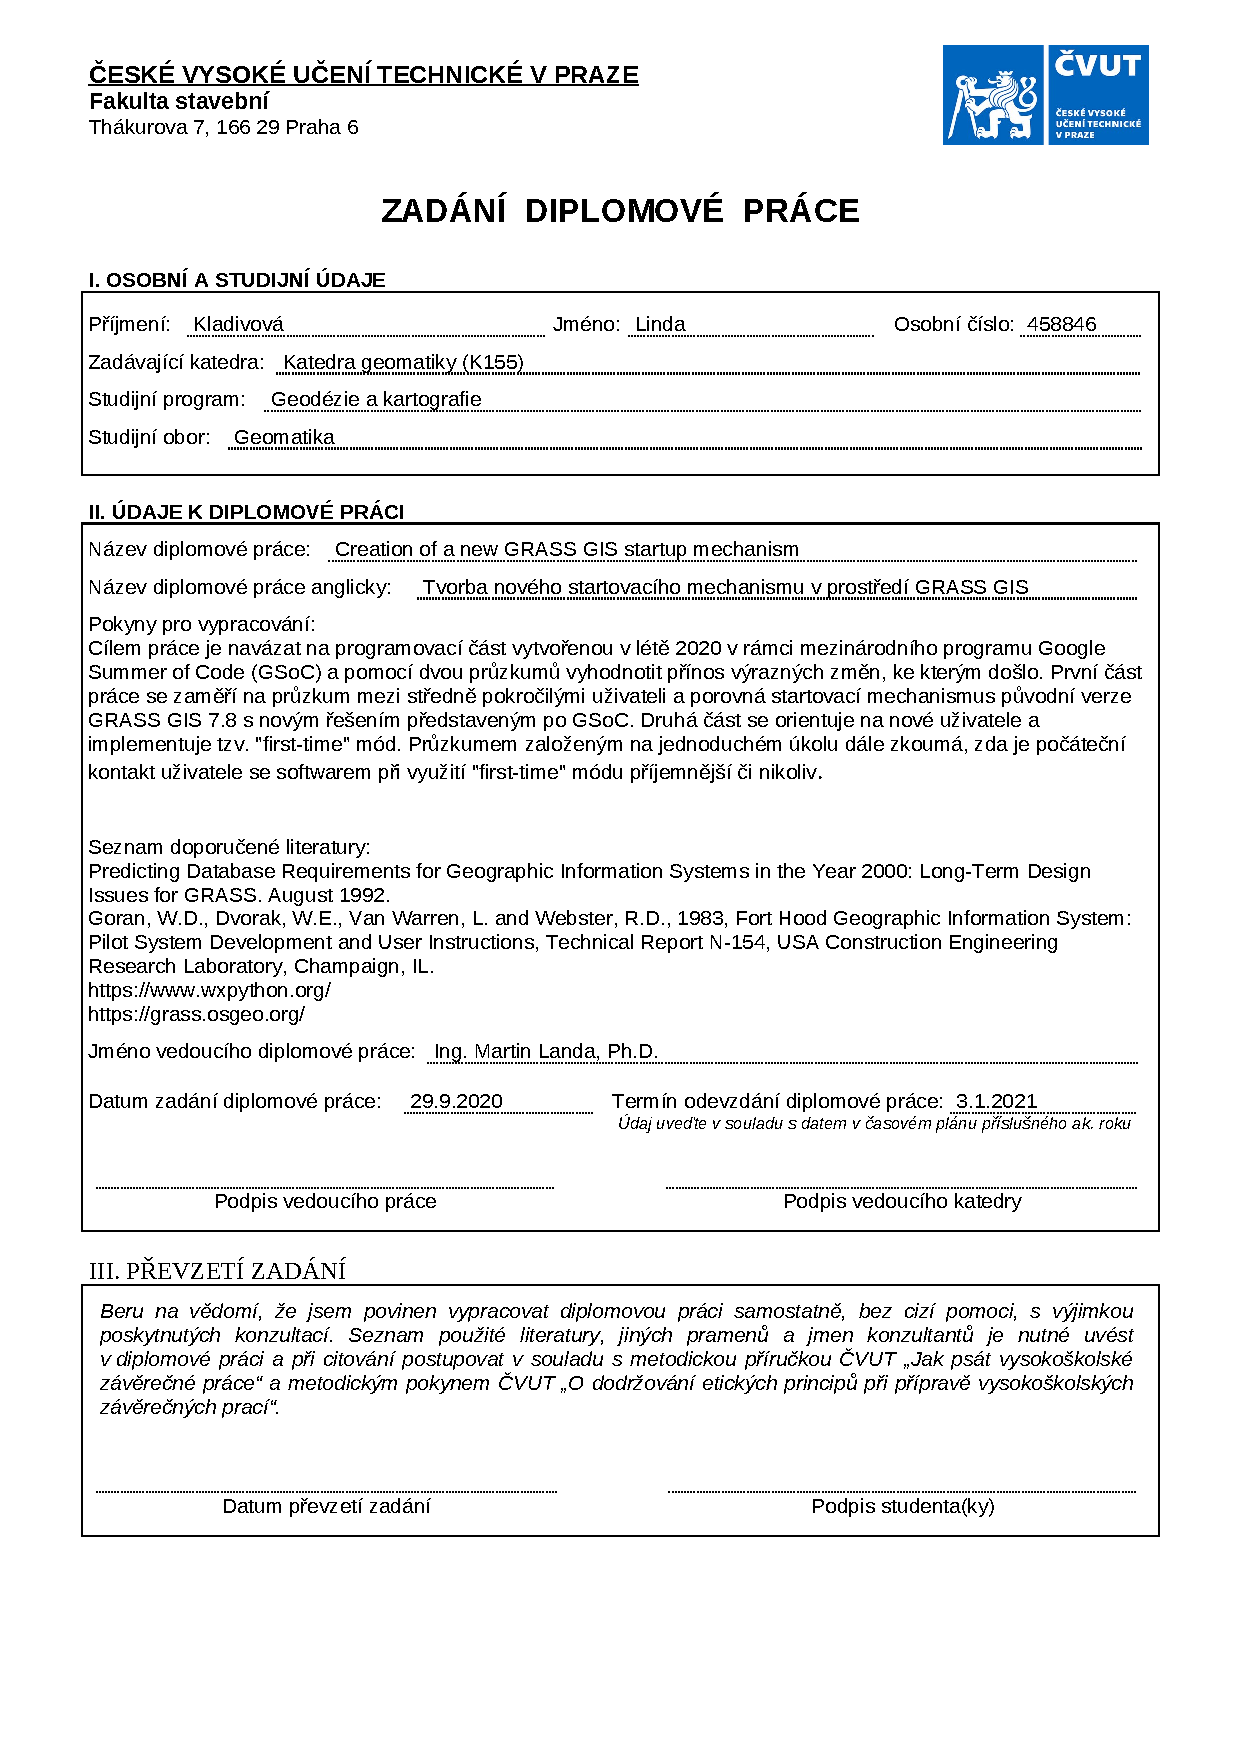
\includepdf[pages=-]{../assignment/zadanidp.pdf}
\end{figure}

%% 4. STRÁNKA ZŮSTANE PRÁZDNÁ

\newpage ~ \newpage
\newpage ~ \newpage
\thispagestyle{empty}

%% 5.  STRÁNKA = ČESKÁ A ANGLICKÁ ANOTACE %%%%%%%%%%%%%%%%%%%%%%%%%%%%%%%%%

\renewcommand{\baselinestretch}{1.2} %zvetseni mezery mezi radky


\begin{Large}
\noindent ANNOTATION
\end{Large}

\large
\noindent
The GRASS GIS startup mechanism could discourage new users from further 
working with this software or at least making it
uncomfortable. This master thesis is built on the programming part
performed in the summer of 2020 within the international Google Summer
of Code program (GSoC) and uses two questionnaires to evaluate the
benefits of significant changes that have taken place. The first part
of the work focuses on a survey among intermediate users and compares
the startup mechanism of the original GRASS GIS 7.8 version with the
new solution introduced after GSoC.  The second part is focused on 
newcomers and implements the special mode for first-time users. 
A survey based on a simple task further examines whether the user's initial 
contact with the software when using the ``first-time'' mode
is more pleasant or not.

\vspace{2ex}
\begin{Large}
\noindent KEYWORDS
\end{Large}

\large
\noindent
\textrm{GRASS GIS, GUI, wxPython, Python, startup, GSoC, first-time user, software development, survey, questionnaire}

\mbox{}
\vfill

\begin{Large}
\noindent ANOTACE
\end{Large} 

\large
\noindent
Dosavadní startovací mechanismus softwaru GRASS GIS mohl odradit nové
uživatele od další práce s tímto softwarem nebo ji alespoň
znepříjemnit. Cílem této práce je navázat na programovací část
vytvořenou v létě 2020 v rámci mezinárodního programu Google Summer of
Code (GSoC) a pomocí dvou průzkumů vyhodnotit přínos výrazných změn,
ke kterým došlo. První část práce se zaměřuje na průzkum mezi středně
pokročilými uživateli a porovnává startovací mechanismus původní verze
GRASS GIS 7.8 s novým řešením představeným po GSoC. Druhá část 
se orientuje na nové uživatele a implementuje tzv. "first-time" mód. 
Průzkumem založeným na jednoduchém úkolu dále zkoumá, zda je počáteční 
kontakt uživatele se softwarem při využití "first-time" módu příjemnější či 
nikoliv.

\vspace{2ex}
\begin{Large}
\noindent KLÍČOVÁ SLOVA
\end{Large}

\large
\noindent
\textrm{GRASS GIS, GUI, wxPython, Python, startup, GSoC, first-time uživatel, vývoj softwaru, průzkum, dotazník}


%% 6. STRÁNKA ZŮSTANE PRÁZDNÁ

\newpage ~ \newpage
\thispagestyle{empty}

%% 7. STRÁNKA = DECLARATION OF AUTHORSHIP %%%%%%%%%%%%%%%%%%%%%%%%%%%%%%%%%

\newpage
\mbox{}
\vfill
\begin{Large}
\noindent DECLARATION OF AUTHORSHIP
\end{Large}

I hereby declare that the work presented here is, to the best of my
knowledge and belief, the original result of my own investigations,
except as acknowledged. All direct or indirect sources used are
acknowledged as references.  \vspace{3ex}

\noindent In Prague ................................... \hfill ................................................

%% 8. STRÁNKA ZŮSTANE PRÁZDNÁ

\newpage ~ \newpage
\thispagestyle{empty}


%% 9. STRÁNKA = ACKNOWLEDGEMENT %%%%%%%%%%%%%%%%%%%%%%%%%%%%%%%%%

\newpage
\mbox{}
\vfill
\begin{Large}
\noindent ACKNOWLEDGEMENT
\end{Large}

First, I would like to thank my parents very much for their support
during my studies. Second, I would like to express my great thanks to
Martin Landa who inspired me a lot on my way to
becoming a professional python developer. In the GRASS GIS 
open-source environment, I met an amazing community of incredibly
inspiring people. Among those people, I would like to thank especially
Anna and Vaclav Petras who were a great support to me during GSoC and
even later on and brought a lot of valuable advice to this
work. Finally, I would like to thank all GRASS users, whether complete
beginners or advanced, who have participated in the questionnaires 
created in this work. They greatly contributed to the decision on how to 
increase the user-friendliness of GRASS GIS. Special thanks go to Pavel Karlovsky 
for his valuable comments on the text of the thesis.


%% 10. STRÁNKA ZŮSTANE PRÁZDNÁ

\newpage ~ \newpage
\thispagestyle{empty}


%% 11. a 12. STRÁNKA = OBSAH A SEZNAM OBRAZKU %%%%%%%%%%%%%%%%%%%%%%%%%%%%%%%%%%
\newpage

\tableofcontents %obsah
\newpage
\listoffigures %seznam obrazku

\thispagestyle{empty}
\newcommand{\obrazek}[1]{(viz obr. \ref{#1})} %specialni reference na obrazek

\newpage
\pagestyle{fancy}

%% NASTAVENI VZHLEDU STRANEK (ZAHLAVI A ZAPATI)

% zajistí, že se názvy kapitol a sekcí nebudou sázet velkými písmeny
\renewcommand{\sectionmark}[1]{\markright{\ #1}}

\fancyhf{} % smaže aktuální nastavení záhlaví a zápatí
\renewcommand{\headrulewidth}{0.4pt} % vrchní linka
\renewcommand{\footrulewidth}{0.4pt}  %  spodní linka
\addtolength{\voffset}{-0.4cm}

 %záhlaví
\fancyhead[LE, LO]{{
\includegraphics[width=1cm]{../pictures/logo_cvut.png} }
   {\textsc{\small {CTU in Prague}} }} %logo skoly
\fancyhead[RE, RO]{\nouppercase{\rightmark}}
   
 %zápatí
\fancyfoot[RO, LE]{{\textsc{\small \thepage}}}

\fancypagestyle{plain}{
  \fancyhead{} % na prázdných stránkách nechci záhlaví
  \renewcommand{\headrulewidth}{0pt} % ani linku
}


%% -------<<< Chapter: Introduction >>>-------\\%%%%%%%%%%%%%%%%%%%%%%%%%%%%%%%%%%%%
\newpage
\vspace*{-1cm}
\pagestyle{fancy}
\fancyhead[RE, RO]{\fancyplain{}{\small \sl{Introduction}}}
\section{Introduction}
\large
\setcounter{page}{17}  % nastaví čítač stránek od stránky Úvod na stránku č. 13

\noindent According to the evaluation of the GIS Geography journal
\cite{gisgeography}, GRASS GIS (Geographic Resources Analysis Support
System) is one of the best software in the world of
open-source software focused on Geographic Information System (GIS) 
in terms of numerical analysis. The history of GRASS, built for vector
and raster geospatial management, geoprocessing, spatial modeling, and
visualization, dates back to 1982 when the United States military started its development..
At the time of writing this thesis, the current 
stable version of the software is version 7.8, but as the number 
suggests, the planned version 8.0, which will be released in the spring
 of 2021, will introduce major changes. They are going to be largely 
 related to the GRASS graphical user interface (GUI).

Although in the startup screen of version 7.8, there is a certain
effort to provide the first-time user with the maximum possible help,
the development community often encountered misunderstandings from the
ranks of users. These complaints led to creating an
% ML: Prague Roadmap could be in quotes, but for sure - reference is missing
% LK: Reference and quotes added 
implementation proposal known as the ``Prague Roadmap'' \cite{roadmap}. 
This proposal was
% ML: GSoC is mentioned many times in the theses (is there reference
% to wiki page somewhere), see 1.2 & 1.4, please add clear reference
the basis for the author's participation in the global Google
% ML: "students into" (skip student developers - what does it mean?)
% LK: word ``student'' removed
Summer of Code program (GSoC) focused on bringing more
developers into open-source software development. The task of GSoC was
to change the sort of unfortunate GRASS startup mechanism so that it
would be easier for first-time users to become familiar with
GRASS. After GSoC changes, the startup screen -- the
% ML: find better word that "trick"
% LK: Changed to ``challenge''
biggest challenge for new users, was partially removed. The primary role for
the data organization was taken over by the Data Catalog -- a tree
object whose functionality was significantly expanded. Now, the
possibilities of managing data hierarchy components are even beyond
the options previously available in the startup screen.
% LK: citation added
The workflow of GSoC participation is described in detail on the 
GRASS wiki page \cite{gsoc}. 

Therefore, this work follows up on the complex topic of creating a
better GRASS GIS startup mechanism. The main part of the work consists
of two surveys, where the first one consists of two parts. The first part aims 
to evaluate the benefits of significant changes
% ML: replace "final" with more suitable word (final is never final;-)
% LK: replaced by suitable
among the GRASS community and at the same time to propose a suitable
% ML: for "existing" user - what does it mean?
% LK:  ``for "existing" user'' removed
solution for the GRASS startup mechanism where
the old startup screen will be permanently removed. The second part of the
first survey focuses on the improvement of the startup mechanism for
first-time users. Already at GSoC, it was decided that some form of
assistance to new users would need to be implemented. The second part
of the survey finds out what options of the first-time help would be
preferred. The second survey conducted one month later introduces a
new special mode for first-time users (so-called ``first-time'' mode), which
extends the default location concept with an infobar helping
users manage the first steps. It examines whether users like the
newly designed mockups of the infobar and gives them space to share
ideas. Based on the analysis of the second survey, the infobar is
improved and subsequently implemented.

\newpage
\vspace*{-1cm}
\subsection{GRASS GIS}
\label{subsection:grassgis}
\noindent GRASS GIS is a cross-platform desktop geographic information
system (GIS) designed to work with geographic 2D/3D raster and vector
data with SQL-based attribute management and vector network analysis.
It supports both the command line and graphical user interface
(GUI). Besides, it offers many spatial modeling algorithms, 3D
visualization, as well as image processing routines pertaining to
LiDAR and multi-band imagery \cite{NETELER2012124}. It is open-source
software published under the GNU GPL general license and managed and
developed under the Open Source Geospatial Foundation
(OSGeo). The GRASS system's influential users include
NASA, NOAA, USDA, USGS, and many environmental consulting companies
\cite{grassgis}.

The power of software stems mainly from its Unix philosophy, where the
software itself consists of a collection of more than 500 applications
called modules. Each of these modules has only one task to perform.
The real power of the software comes when the various of these
modules begin to chain together, allowing the user to create even very
complex applications. Most of these modules are written in C. However,
above the whole system, PyGRASS as an object-oriented Python
Application Programming Interface (API) stands, which hides the
complexity of GRASS and provides access to the C-API capability
of GRASS for geoscientists that are not familiar with C
\cite{pygrass}.

% ML: GRASS is using versioning system since 1999 (CVS, than
% Subversion). 
% LK: proposed sentence added 
GRASS GIS had been using the versioning system since 1999 (CVS, then
Subversion). Since January 2020, it has been developing on GitHub, a web
version control using Git. Nowadays, most main changes take place in
the Python language. For GUI coding, wxPython GUI toolkit is used.
% ML: extension -> library (or better GUI toolkit)
% LK: changed to GUI toolkit
Besides improving the GRASS GIS startup mechanism,
in summer 2020, the community presented a new website (see Figure
\ref{fig:grass_gis}) on the occasion of its 37th birthday, which offers
a curated list of tutorials in different languages and links to
videos.

\vspace{0.7cm}
\begin{figure}[hbt!]
\begin{center}

\includegraphics[width=17cm]{../pictures/grass_gis.png} 
\caption[New GRASS website's layout]{New GRASS website's layout (Source: \cite{grass})}
\label{fig:grass_gis}
\end{center}
\end{figure}

\newpage
\vspace*{-1cm}
\subsubsection{Data hierarchy in GRASS GIS}
\label{subsection:hierarchy}
\noindent
\large

\noindent While in other GIS software it is usually customary to store
work in so-called \textit{projects} containing \textit{map layers},
GRASS GIS keeps its unique data hierarchy, which has proven very
useful over the years, especially for experienced users. Every GRASS
GIS user has undoubtedly come across the following terms: Database,
Location, Mapset, and Maps. These four representations form a tree of
rules, which we can see in Figure \ref{fig:grass_data_hierarchy}.

\vspace{0.3cm}
\begin{figure}[hbt!]
\begin{center}
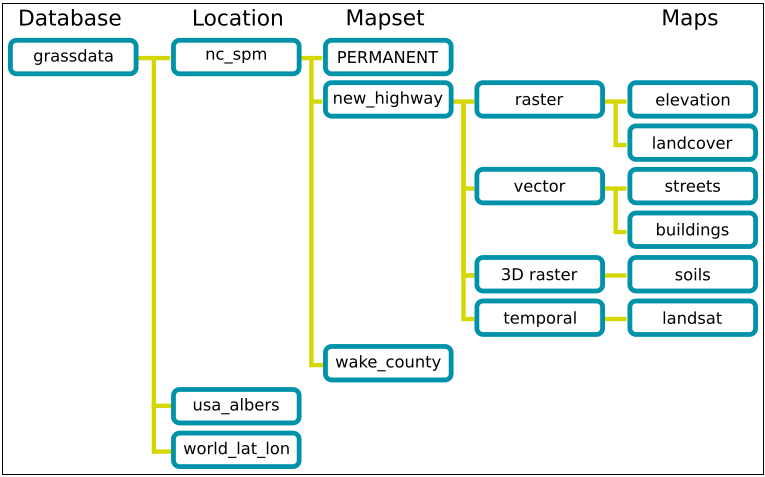
\includegraphics[width=14cm]{../pictures/grass_data_hiearchy.png} 
\caption[GRASS GIS 7 location structure]{GRASS GIS 7 location structure (Source: \cite{hierarchy})}
\label{fig:grass_data_hierarchy}
\end{center}
\end{figure}

\noindent The Database, which is built hierarchically at the top, has
the character of a base directory, whose usual name is
``grassdata''. It contains Locations -- collections of data with a
common coordinate reference system (CRS). Therefore, Maps in the
Mapsets contained in a particular Location will always have the same
coordinate system.

It is also important to mention that a
mapset named PERMANENT is automatically created when creating a location. Briefly speaking, the
PERMANENT mapset is used to store general spatial data, which are also
accessible but write-protected to other users who are working in the
same Location as the Database owner. The PERMANENT mapset also holds
% ML: not only extent, but also resolution ("computational region" in GRASS terminology)
% LK: ok
the default region boundary coordinate values and resolution 
("computational region" in GRASS terminology). 
This is important for raster analysis \cite{hierarchy}.

In the following text, the GRASS data hierarchy elements are
already taken as standard terms, and the initial letters are lowercase.

\newpage
\vspace*{-1cm}
\subsection{State of Art before GSoC}
\label{sec:beforeGSoC}

\noindent Since the GRASS GIS version 7.8 (before GSoC) has
considerably complicated setup, we need to define what the term
\textit{startup mechanism} means in connection with GRASS. It
basically includes three things:

\begin {itemize}

\item the way GRASS GIS can be started. In the case of a Unix
  operating system, it is run from the command line.

\item GUI (graphical user interface) components that the user
  encounters during startup. In the case of GRASS GIS version 7.8,
  these are the splash screen, startup screen, and Location
  Wizard. There may be situations where the requested mapset is locked
  (this happens if it is used by another process, or if the last
  session in this mapset ended in an error). If the running mapset is
  locked, we are first notified that there is a lock file with a
  .gislock extension in the mapset, and then asked if we want to
  delete this file. In this special situation, when running GRASS, we
  even encounter five different GUI components.  In the case of the
  version after GSoC, the mentioned components are bypassed in most
  situations and we can move straight to the third point.

\item the state instantly after startup -- here we can talk e.g. about
  the state of individual Layer Manager tabs, and Map Display.

\end{itemize}

\noindent As we could notice, there are several GUI components that
need to be clarified at the outset. Let's first look at the role of
the individual GUI components in version 7.8 (before GSoC). Due to
significant changes, the author of this work made during the GSoC, the
role of the startup screen and Data Catalog in version after GSoC
is very different compared to version 7.8. The Data Catalog takes over
the role of the startup screen. The state after GSoC is clearly
described in section \ref{sec:afterGSoC}. The author evaluates
the benefits of the changes in Survey 1 Part 1. In
both subsections \ref{sec:beforeGSoC} and \ref{sec:afterGSoC}, the
GRASS GUI software components are arranged chronologically according
to the order in which the user encounters them.

\bigskip
\noindent \textbf {Startup screen versus splash screen}

\noindent As Ed Foster stated in 1996 \cite{foster}: ``Splash screens,
as they are commonly called, are the graphic logos that display while
the program is loading and identify the program while reminding you
about the software publisher's copyright restrictions." So, it appears
before the main software window starts and remains visible for a few
seconds. If we try to find articles on the startup screen, we will not
be very successful. Nowadays, this topic lives mainly on programming
websites such as Stack Overflow. In some software, a startup screen can
mean at the same time a splash screen if no other startup screen
appears (among GIS software e.g. gvSIG, SAGA GIS). However, generally
speaking, a startup screen usually requires some initial action from
the user to set up the software.

The startup screen is the first component of the GRASS GIS version 7.8
% ML: "meet" doesn't sound good, try better wording
% LK: changed to ``encounter''
that the user encounters. It allows us to set all the above-mentioned components
except maps and, in the case of locations and mapsets, also manage
them in terms of renaming and deleting. The various historical
versions of the startup screen can be seen in Figure
\ref{fig:verze_startup}. The one on the right corresponds to the version
7.5 (as well as 7.8).

%% ML: source?
% LK: source added
\vspace{0.3cm}
\begin{figure}[hbt!]
\begin{center}
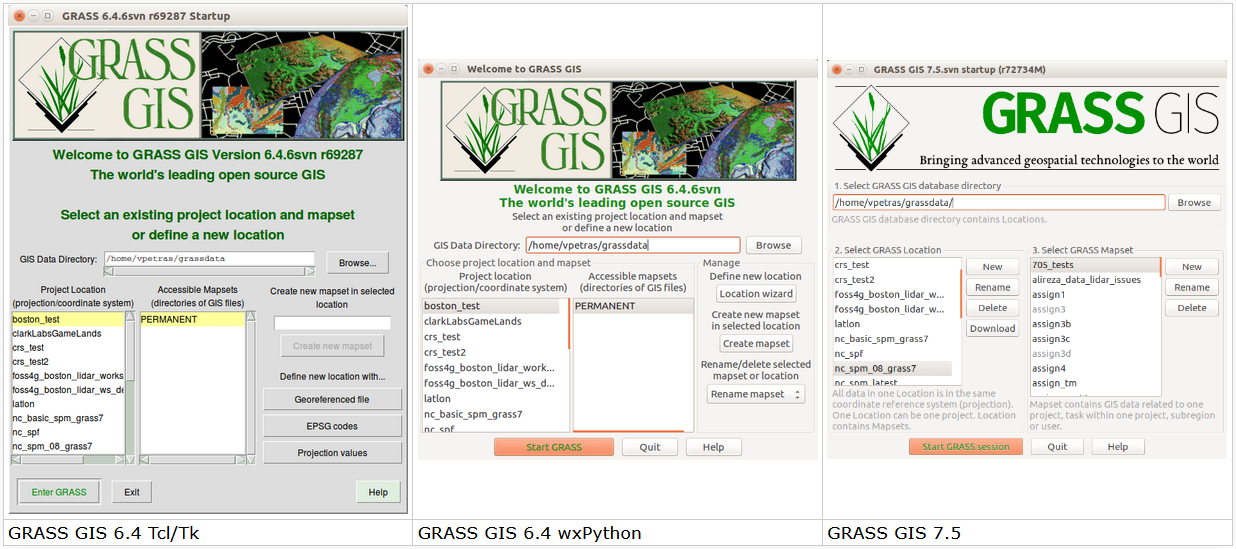
\includegraphics[width=17cm]{../pictures/verze_startup.png} 
\caption[Historical versions of GRASS startup screen]{Historical versions of GRASS startup screen (Source: \cite{intro})}
\label{fig:verze_startup}
\end{center}
\end{figure}

\bigskip
\noindent \textbf {Location Wizard}

\noindent Location Wizard is a software component, which has the
character of a guide that appears when creating a new
location. Therefore, the main task of the wizard is to define the
Coordinate Reference System (CRS). It consists of four consecutive
dialog boxes (the third box can be seen in Figure \ref{fig:loc_wizard_sour_pred}). A comparison of the Location Wizard before and after
GSoC is included in subsection \ref{sec:afterGSoC}.

\bigskip
\noindent \textbf {Layer Manager and Map Display}

\noindent The peculiarity of GRASS GIS is that it does not consist of
one software window, as is usually the custom, but directly of
% ML: in section header you mentioned 'Map Display', keep terminology consistent (Display vs Window)
% LK: changed
two. The topic of connecting Layer Manager with Map Display is, by the
way, one of the proposed topics on GSoC
\footnote{\url{https://trac.osgeo.org/grass/wiki/GSoC/2020\#GRASSGUI:Singlewindowlayout}}.
As explained in more detail in the GRASS documentation, the
Layer Manager provides a GUI for creating and managing maps. In Figure
\ref{fig:empty_layers1} we can notice five tabs -- Layers, Console,
Modules, Data, and Python.

\vspace{0.3cm}
\begin{figure}[hbt!]
\begin{center}
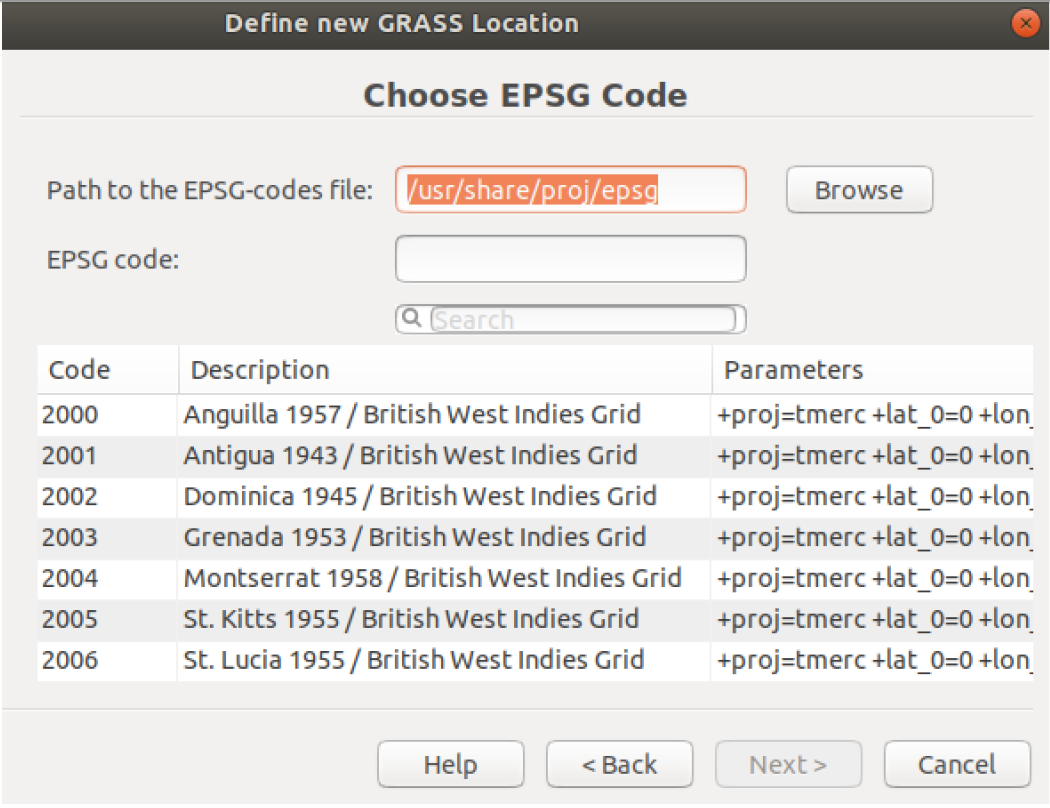
\includegraphics[width=11.5cm]{../pictures/loc_wizard_sour_pred.png} 
\caption[Choosing EPSG code in Location Wizard in version 7.8]{Choosing EPSG code in Location Wizard in version 7.8 (Source: Personal collection)}
\label{fig:loc_wizard_sour_pred}
\end{center}
\end{figure}

\noindent  In the Layer Manager version 7.8, after
% LK: maps in brackets
running GRASS we first see the Layers tab, which allows layers (maps) in Map
Display to be switched on and off. After starting the session this tab
is empty. The path to the current mapset and location can be noticed
in the top bar in the Map Display window. In this case, the current
% ML: demomapset in italics(?)
% LK: ok
mapset is called \textit{demomapset} and is located in the location named
\textit{fire\_grassdata}. GRASS GIS allows adding more Map Display
% ML: at beggining of this paragraph you are using "maps" term, now
% "layers". This need to be explained, kept consistent.
windows. We can then manage layers in these windows via the Layers
tab.

\vspace{0.3cm}
\begin{figure}[hbt!] 
\begin{center}
  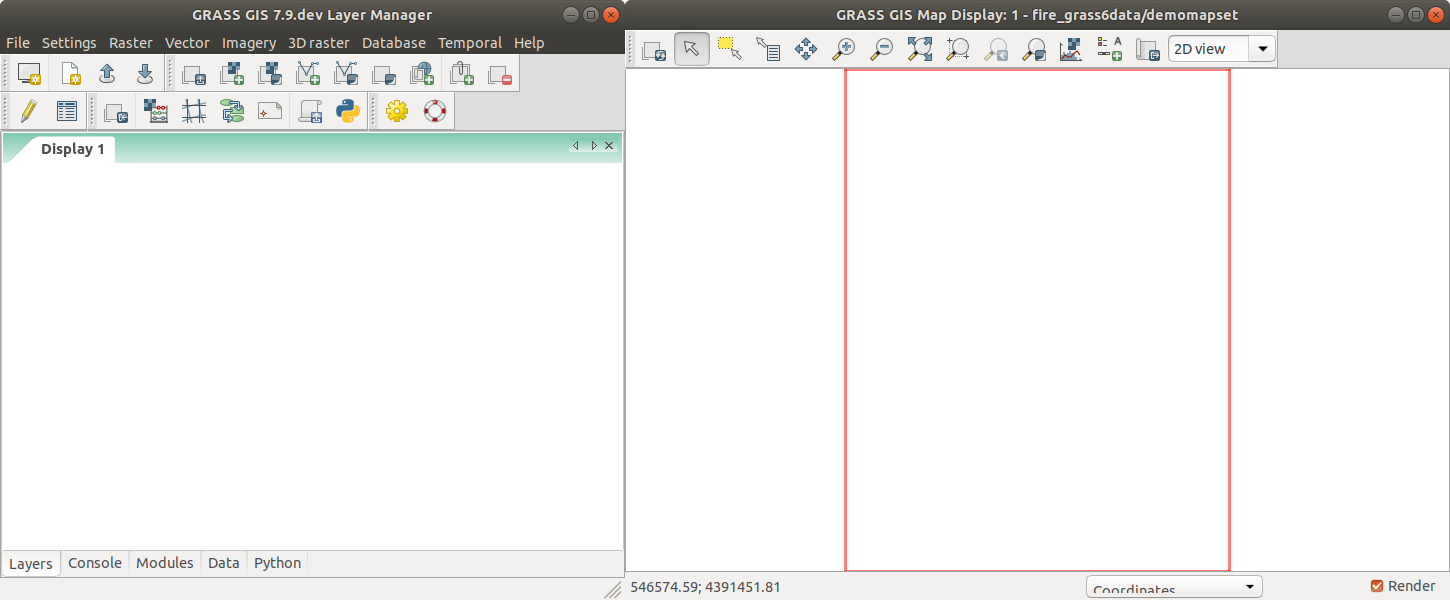
\includegraphics[width=17cm]{../pictures/empty_layers1.png}
  % ML: Window vs Display
  % LK: ok
\caption[Layer Manager and Map Display in version 7.8]{Layer Manager and Map Display in version 7.8 (Source: Personal collection)}
\label{fig:empty_layers1}
\end{center}
\end{figure}

\noindent In this work we will deal only with the Data tab, the
explanation of other tabs can be found in the documentation
\footnote{\url{https://grass.osgeo.org/grass79/manuals/wxGUI.html}}.
 
\bigskip
% LK: rewrited
\noindent \textbf {Data tab}

\noindent The Data tab  in Figure \ref{fig:data_catalog_pred} contains 
two objects -- the Data Catalog (data hierarchy tree)
and the toolbar, which allows e.g. updating and searching in the tree.

The Data Catalog enables to display the data located in the 
\textit{current location} (equal to active location). Within the 
Data Catalog we are allowed to work with maps through
the context menu - to display, rename and delete them, display their
metadata, or to copy them from another mapset. However, the Data Catalog
in version 7.8 does not provide management of mapsets, locations, or a
database. This management is sort of hidden in the Settings/GRASS
working environment menu.

The data in the current location are firmly connected to the Map Display
window. If we want to see maps from a different location we can find in
the mapset context menu the option for switching. We are able to
switch between mapsets in the same location or between mapsets in
different locations. If we copy the data to the mapset in another
location with a different CRS, the projection takes place. GRASS GIS
does not use the ``on the fly'' transformation.

%% ML: not limited only to current (you can display all data from
%% current location)
%%
%% ML: Data catalog is not the only way how to display data ("we need
%% to go"), https://training.gismentors.eu/grass-gis-zacatecnik/intro/zobrazeni-geodat.html
%\textit{current mapset} (equal to active mapset), we need to go to the
%% ML: try to rewrite sentence "In this tab" (you are not speaking
%% about "tab" before)
%Data tab. In this tab provided in Figure \ref{fig:data_catalog_pred},
%there is a Data Catalog in the middle, and the toolbar in the upper
%% ML: "we are" sounds strange in this context
%part. Within the Data Catalog we are allowed to work with maps through
%the context menu - to display, rename and delete them, display their
%% ML: usually "*from* another mapset"
%metadata, or to copy them from another mapset. However, the Data Catalog
%in version 7.8 does not provide management of mapsets, locations, or a
%database. This management is sort of hidden in the Settings/GRASS
%% ML: it's not tab, but the menu.
%working environment menu.

%% ML: why "in the current mapset"?, you can read/display data also from
%% other mapsets
%%
%% ML: "what means "firmly" in this context?, the whole paragraph
%% doesn't make sense to me - probably you meant "current location"
%% instead of "current mapset"?
%% ML: please rewrite whole paragraph - it's very confusing
%The data in the current location are firmly connected to the Map Display
%window. If we want to see maps from a different location we can find in
%the mapset context menu the option for switching. We are able to
%switch between mapsets in the same location or between mapsets in
%% ML: how you can move mapset to another location via GRASS GUI/CLI?
%% It's not possible and not allowed
%different locations. If we move the data to the mapset in another
%%% ML: the last sentence is the only correct
%location with a different CRS, the projection takes place. GRASS GIS
%does not use ``on the fly'' transformation.

\vspace{0.3cm}
\begin{figure}[hbt!] 
\begin{center}
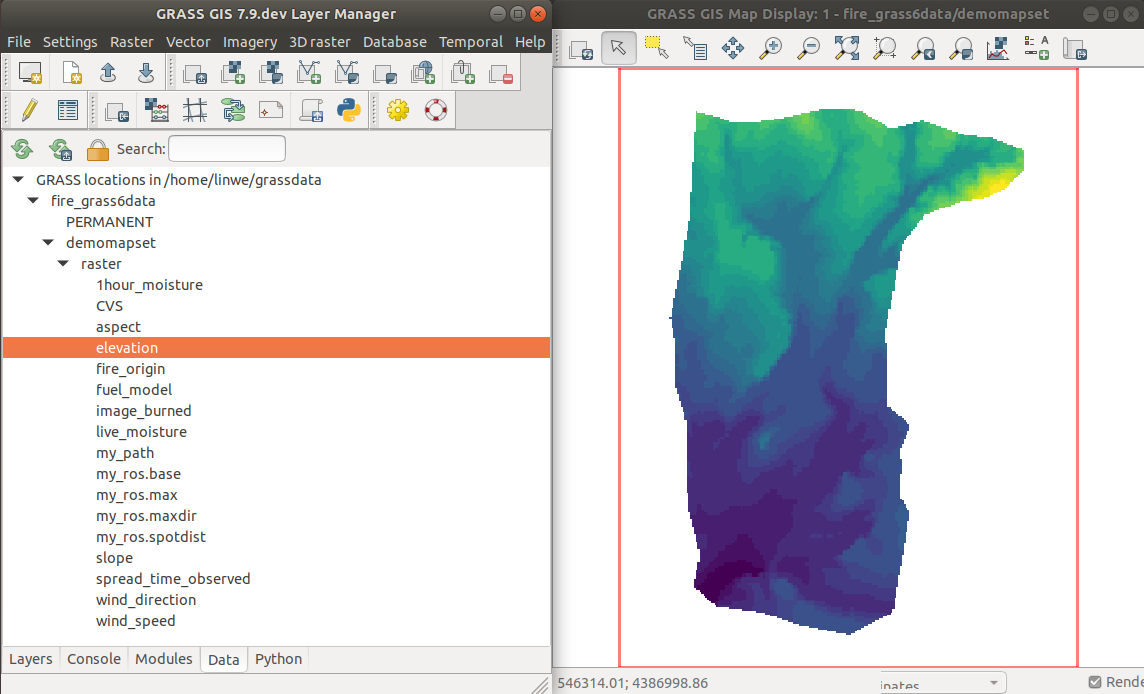
\includegraphics[width=16cm]{../pictures/data_catalog_pred.png} 
\caption[Data Catalog in version 7.8]{Data Catalog in version 7.8 (Source: Personal collection)}
\label{fig:data_catalog_pred}
\end{center}
\end{figure}

\newpage
\vspace*{-1cm}
\subsection{Prague Roadmap}
\label{section:Prague Roadmap}
\noindent
\large The data hierarchy described in subsubsection
\ref{subsection:hierarchy} proves its worth especially when used by
experienced users of GRASS, however, for complete beginners, it is
rather confusing. Especially if the above-mentioned main components
(database, location, and mapset) have to be defined right at the start
% ML: try to find better word than "standard"
% LK: changed
of the software in the startup screen, which is used since
version 6.4.  Although, in the startup screen of version 7.8, there is
a certain effort to provide the first-time user with the maximum
possible help (short description of data hierarchy, ``Help'' button), the
development community often encountered misunderstanding from the
ranks of users
\footnote{\url{https://trac.osgeo.org/grass/ticket/3474}}. The
disadvantages of GRASS mentioned in the evaluation of the GIS Geography
journal \cite{gisgeography} are also largely related to the current
startup mechanism. According to this source, the main disadvantage of
GRASS version 7.8 is mainly the clunky and dated user interface,
defining projects on start-up and a steep learning curve to get started.

The general question, on which answer the community has still not
fully agreed over the years, is whether to keep existing data
hierarchy at all or change the whole concept and use only
\textit{project} and \textit{map} terms, which is the usual standard
for other GIS software. The \texttt {database/location/mapset}
mechanism may indeed seem complicated at first glance, but we must
keep in mind that many later problems will be avoided by clearly
defining the CRS at the beginning and allowing only one coordinate
% ML: here we are not directly speaking about GRASS, right? So
% "location" -> "project" ?
% LK: yes thats true, changed
system within one project. From the author’s point of view, the
advantage (perhaps from the point of view of first-time users maybe
the disadvantage) is that GRASS GIS does not support ``on the fly''
transformation which shows differently projected data in the right
place on the map. It guarantees that we cannot analyze data having a
different coordinate system together, as could happen in ArcGIS or
QGIS, for example. In GRASS GIS, we also cannot get into a situation
that ``on the fly'' transformation does not occur at all, but despite
this, it is allowed to display two layers of different coordinate
systems on top of each other. This, of course, results in the
incorrect rendering of the layers in the map window (may happen
e.g. in SAGA GIS).

In 2017, the first suggestions on how to simplify this startup screen
began to appear. In terms of implementation complexity, the simplest
and most effective proposal seemed to be proposal A3
\footnote{\url{https://trac.osgeo.org/grass/wiki/wxGUIDevelopment/New\_Startup\#ProposalA3Prague2019:Datatreeandbigbuttons}}. Based
on this proposal, the implementation proposal known as the Prague
Roadmap\footnote{\url{https://trac.osgeo.org/grass/wiki/wxGUIDevelopment/New\_Startup\#PragueRoadmap}}
was created in 2019 in Prague.  The most serious changes concern the Data Catalog. They lie in supporting multiple
databases, adding buttons to create existing or new databases, or
adding new actions from the context menu to a database, location, and
mapset node. Considering the disadvantages mentioned in the paragraph
above, it was decided (August 31, 2020, unpublished video
call) that the data hierarchy \texttt{database/location/mapset} will be
preserved. 
%In addition, this proposal introduces a new concept called
%% ML: Workspace files has been introduced to GRASS much more earlier
%% (before 7.4 for sure)
% LK: ok, the sentence is not used
%\textit{workspace} which is not directly part of a mapset, but is
%associated with it.


%%% ML: to be reviewed - start
%%% ML: Done
\noindent The proposed changes in the Location Wizard are mainly related to the
clarification of the first page, better naming of the given
attributes, and speeding up the selection of the coordinate system in
% ML: Explain idea of using Data Catalog in startup screen in more
% understandable way (Data Catalog is already used in the GUI, here it
% was planned to use it also for startup screen purposes)
the dialog. 

% LK: new paragraph about Data Catalog
The same Data Catalog implemented in the Data tab is
planned to be used within a startup screen. 
The proposal assumes the possibility of
filtering in the Data Catalog based on the recently selected
% ML: what means recetly used "maps" for startup?
items. General startup GUI should be able to collect recently used mapsets and
% ML: twice used "workspace" in a single sentence, you probably meant
% "location" (at the end)
as well as databases and locations. 
% ML: launches for the first time
When GRASS GIS  launches for the first time, the "grassdata" working directory for
storing locations, mapsets and maps should be automatically created in
a reasonable place.

% ML: ah, here you explain the how idea - separate text about location
% wizard and data catalog startup screen usage into two seperate
% paragraphs

To sum it up, the startup screen proposed in Prague Roadmap consists of only one 
startup page, which has a Data Datalog in the center, and a toolbar 
with big buttons for creating or defining new or existing data 
components, such as a location or mapset. There is not any image available
for that design, however, it follows very closely the previous proposal A2 
\cite{A2} created by  Garrett C. Millar, which we can see in Figure 
\ref{fig:roadmap_proposal}.
%%% ML: to be reviewed - end

% ML: you could probably add image from wiki page describing whole
% concept (if there is any)
% LK: figure added
\vspace{0.3cm}
\begin{figure}[hbt!] 
\begin{center}
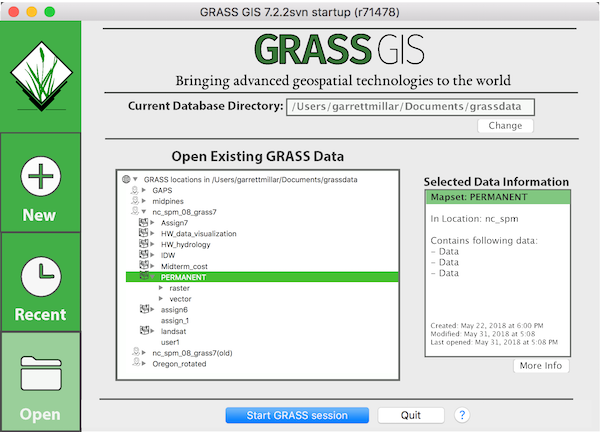
\includegraphics[width=12cm]{../pictures/roadmap_proposal.png} 
\caption[Proposal A2 (Gcmillar): Quick access through well-designed tabs on the side]{Proposal A2 (Gcmillar): Quick access through well-designed tabs on the side (Source: \cite{A2})}
\label{fig:roadmap_proposal}
\end{center}
\end{figure}

\newpage
\vspace*{-1cm}
\subsection{State of Art after GSoC}
\label{sec:afterGSoC}

\noindent The changes that occurred during the GSoC
are fundamental. At first, developers did not plan to remove the
% ML: try to use shorter sentences (long sentences dicreaces
% readibility)
startup screen. The changes were to be based on Proposal A3, which 
suggested that the same Data Catalog, which is available in the 
Data tab after starting the session, will be part of the startup screen. 
During the implementation, however, all the functionality of the startup screen,
including switching mapsets as well as locations and databases, was
% ML: moved -> implemented
% LK': ok
implemented to the Data Catalog, so it no longer made sense to keep this
notion. At least definitely not the form in which it is in version
7.8.

\bigskip
\noindent \textbf {Data Catalog}

\noindent The main goal of GSoC was to improve the Data Catalog in
such a way that enables a user-friendly organization of work. This is
mainly about creating, renaming, and deleting mapsets and locations,
% ML: not only startup screen, but also by Layer Manager's menu
% LK: added
which was previously possible through the startup screen and through 
Layer Manager's menu. However, completely new possibilities have 
been added. In Figure \ref{fig:function} we can see the all
functionalities that have been newly implemented in the Data Catalog.

\vspace{0.3cm}
\begin{figure}[hbt!] 
\begin{center}
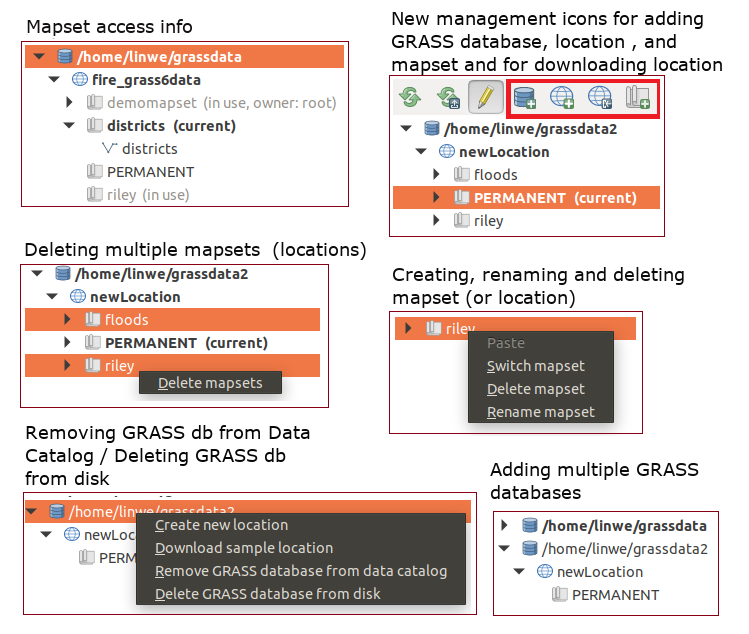
\includegraphics[width=13cm]{../pictures/funkce.png} 
\caption[New functionalities in Data Catalog]{New functionalities in Data Catalog (Source: Personal collection)}
\label{fig:function}
\end{center}
\end{figure}

\noindent GRASS GIS after GSoC allows a user
% ML: add -> work/define (?)
% LK changed to define
to define multiple databases. New management icons in the upper toolbar offer intuitive
creation of the mentioned data components. In the context menu, there
are also new options for deleting several mapsets or
locations. Though, probably the most visible changes are those related
to the graphical representation of the Data Catalog. Next to the
individual components, we can notice small icons distinguishing types
of data hierarchy components. The Data Catalog also informs about
access to individual mapsets (current, in use, and a different
owner). 

Another important thing is related to access to individual
mapsets. In version 7.8, the startup screen informs about the lock and
asks if the user wants to remove the lock. In order to completely take
over the startup screen functionality by the Data Catalog, it is also
% ML: "they" ? try to rewrite the sentence
%% ML: OK
necessary to warn the user that the mapset to which they are going to
switch is locked. How this case was solved is clear from Figure
\ref{fig:data_catalog_switch_new}. Because mapset locking was often
confused with prohibiting editing outside the current mapset, the term
was changed to \textit{mapset in use}. This term can also be seen in
the Mapset Access Info in the Data Catalog.

\vspace{0.3cm}
\begin{figure}[hbt!] 
\begin{center}
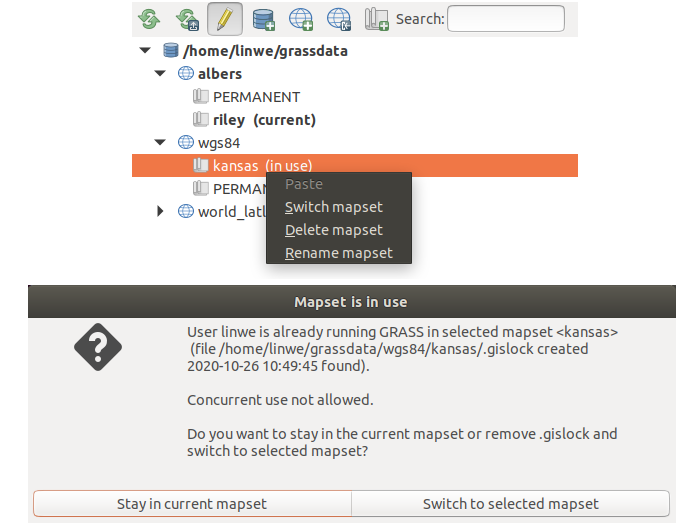
\includegraphics[width=13cm]{../pictures/data_catalog_switch.png} 
\caption[Switching to mapset in use in Data Catalog]{Switching to mapset in use in Data Catalog (Source: Personal collection)}
\label{fig:data_catalog_switch_new}
\end{center}
\end{figure}

\noindent Another substantive step forward was the graphic change of the icon
enabling or disabling changes outside the current mapset. This icon
has newly the bitmap of a pencil (instead of a bitmap of a lock in
version 7.8) and protects a user from unwanted changes. If we do not enable
editing, we cannot rename or delete any mapsets,
% ML: layers -> maps (better data elements - it's more generic, in the
% future data catalog could show also spacetime datasets and other
% data elements, not only raster/vector maps)
locations, and databases. We can only work with data elements inside the
% ML: probably describe short why PERMANENT mapset cannot be deleted
current mapset. (The term ``data elements'' is  more generic, in the
future Data Catalog could show also spacetime datasets and other
data elements, not only raster/vector maps). However, even if we 
enable editing, we cannot delete a PERMANENT mapset. 
Similarly, we are not allowed to delete boldly marked
\textbf{current} components in the Data Catalog.

\bigskip
\noindent \textbf {Location Wizard}

\noindent This guide to creating new locations has been slightly
modified and streamlined. In particular, we can see it on the first
page ``Define a new GRASS location'' in Figure
\ref{fig:loc_wiz_1}. Checkboxes and simplified names are removed
here. Furthermore, the GRASS database can be modified.

\begin{figure}[hbt!] 
\begin{center}
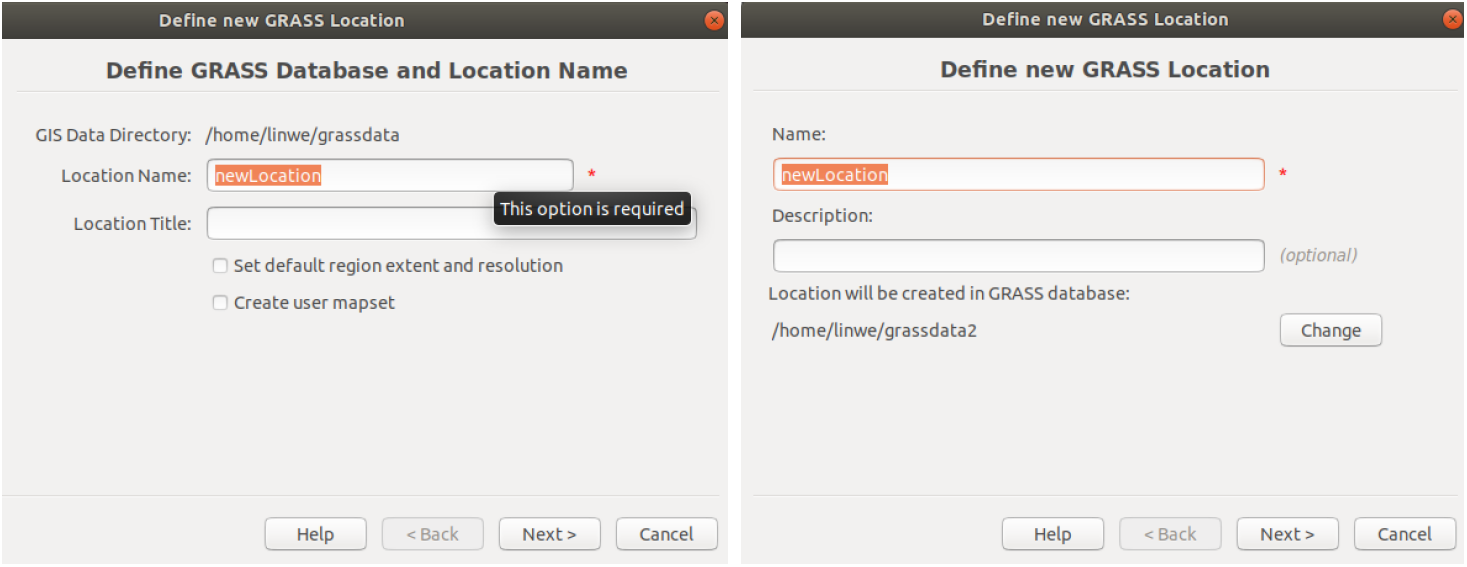
\includegraphics[width=15.5cm]{../pictures/loc_wiz_1.png} 
\caption[Location Wizard first page before and after GSoC]{Location Wizard first page before and after GSoC (Source: Personal collection)}
\label{fig:loc_wiz_1}
\end{center}
\end{figure}

\noindent The second page is renamed to ``Select Coordinate Reference
System (CRS)''. As we can see in Figure \ref{fig:loc_wiz_2}, the
division into simple and advanced methods is abolished in the new
version. Besides, CRS can be newly specified using a WKT string.

\begin{figure}[hbt!] 
\begin{center}
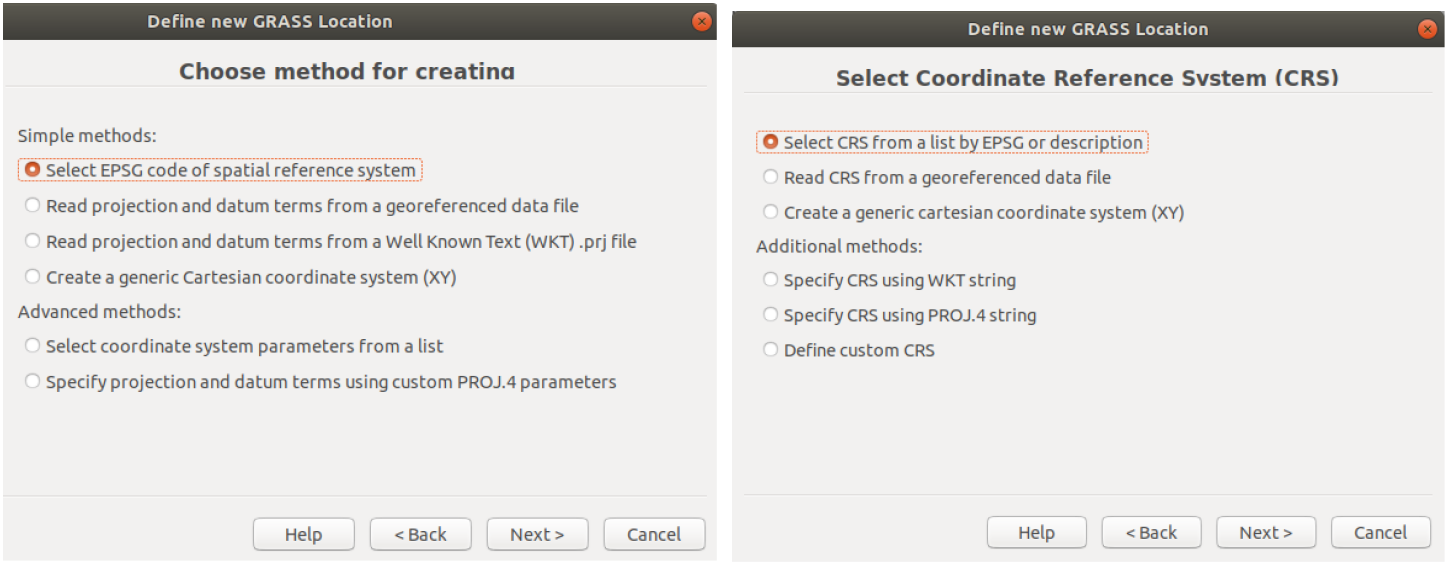
\includegraphics[width=15.5cm]{../pictures/loc_wiz_2.png} 
\caption[Location Wizard second page before and after GSoC]{Location Wizard second page before and after GSoC (Source: Personal collection)}
\label{fig:loc_wiz_2}
\end{center}
\end{figure}

\noindent  However, the essential change is related to the ``Choose
EPSG code'' page. Now it supports dynamic EPSG search and the
hyperlink which is changed dynamically according to a filter set by an
user (see Figure \ref{fig:loc_wiz_3}). The last page of the Location
Wizard called ``Summary'' remains unchanged.

\begin{figure}[hbt!] 
\begin{center}
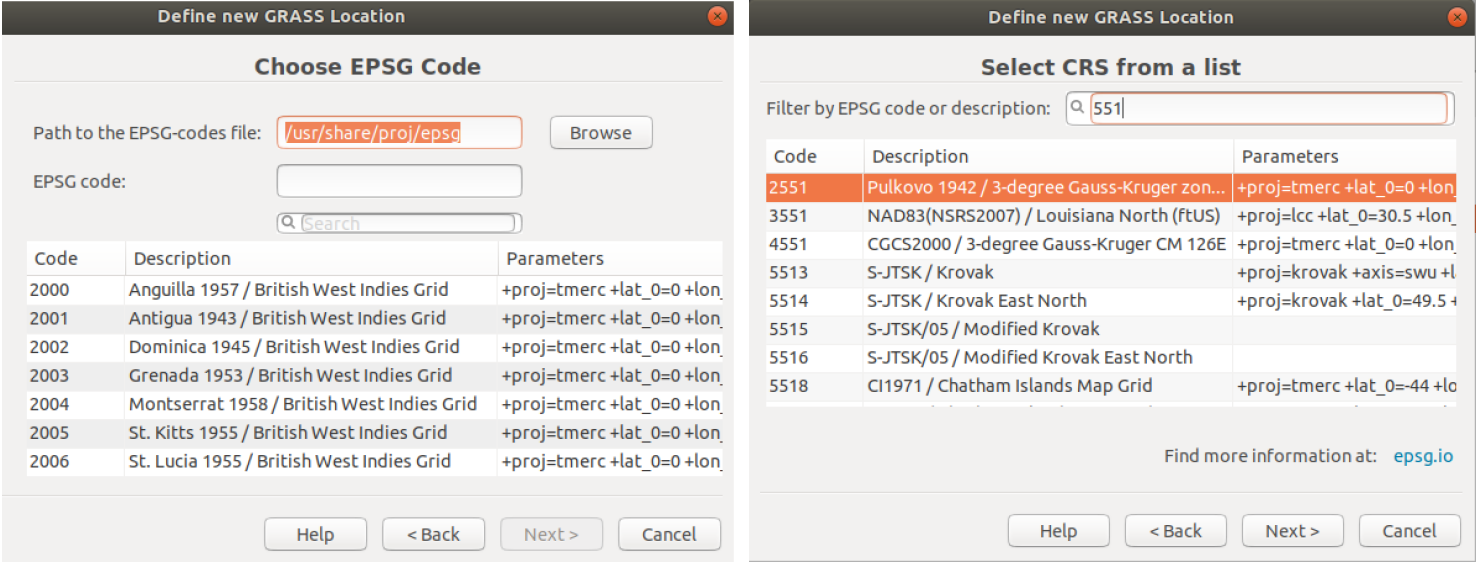
\includegraphics[width=17cm]{../pictures/loc_wiz_3.png} 
\caption[Location Wizard third page before and after GSoC)]{Location Wizard third page before and after GSoC (Source: Personal collection)}
\label{fig:loc_wiz_3}
\end{center}
\end{figure}

\bigskip
\noindent \textbf {Startup screen}

\noindent We can encounter three different situations when starting
the GRASS GIS ``after GSoC'' development version:

\begin{enumerate}

\item \textbf{GRASS bypasses the startup screen and starts in the
    pre-prepared default location (also ``demolocation'' in
    development slang)} (see Figure
  \ref{fig:demolocation_startup}). This situation occurs after the
  software is installed, that is when no used databases are stored in
  the settings. The default location called
  \textit{world\_latlong\_wgs84} in WGS84 coordinate system
  (EPSG:4326) shows the correct organization of the data. Base data
  are stored in a PERMANENT mapset whereas already analyzed data
  belongs to another mapset, for example to the one named after a
  user. The current implementation does not show the World map
  included in \textit{country\_boundaries} layer immediately at
  startup, it is necessary to display the map using Data Catalog (see
  Figure \ref{fig:demolocation}). The splash screen does not appear.
\item\textbf{ GRASS bypasses the startup screen if possible to start
    in the last used mapset} (see Figure
  % ML: from text it's not clear that GRASS starts in the last used
  % location/mapset
  % LK: added
  \ref{fig:last_mapset_startup}). The situation when GRASS starts in 
  the last used location/mapset is probably the most common. 
  The software remembers the databases that were open when the
  last session was closed and opens them.  The splash screen does not
  appear.
  % ML: if the last used mapset ...
  % LK: added
\item \textbf{GRASS launches in startup screen if the last used mapset
 is not in a usable state} (was deleted or is used by another process). 
 In this special situation, GRASS starts in the same way as in version 7.8.

\end{enumerate}

\vspace{0.3cm}
\begin{figure}[hbt!] 
\begin{center}
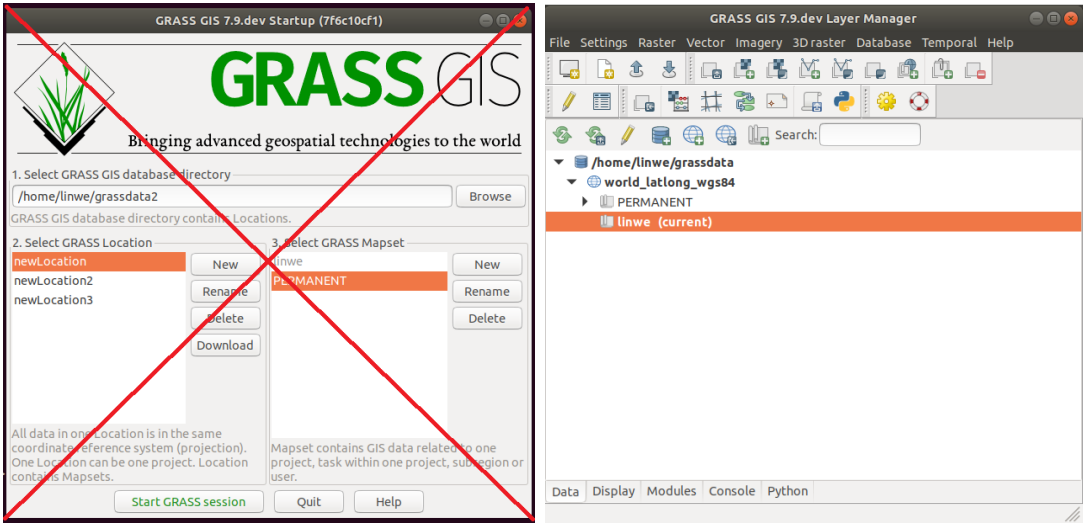
\includegraphics[width=17cm]{../pictures/demolocation_startup.png} 
\caption[GRASS starts in the pre-prepared default location]{GRASS starts in the pre-prepared default location (Source: Personal collection)}
\label{fig:demolocation_startup}
\end{center}
\end{figure}

\vspace{0.3cm}
\begin{figure}[hbt!] 
\begin{center}
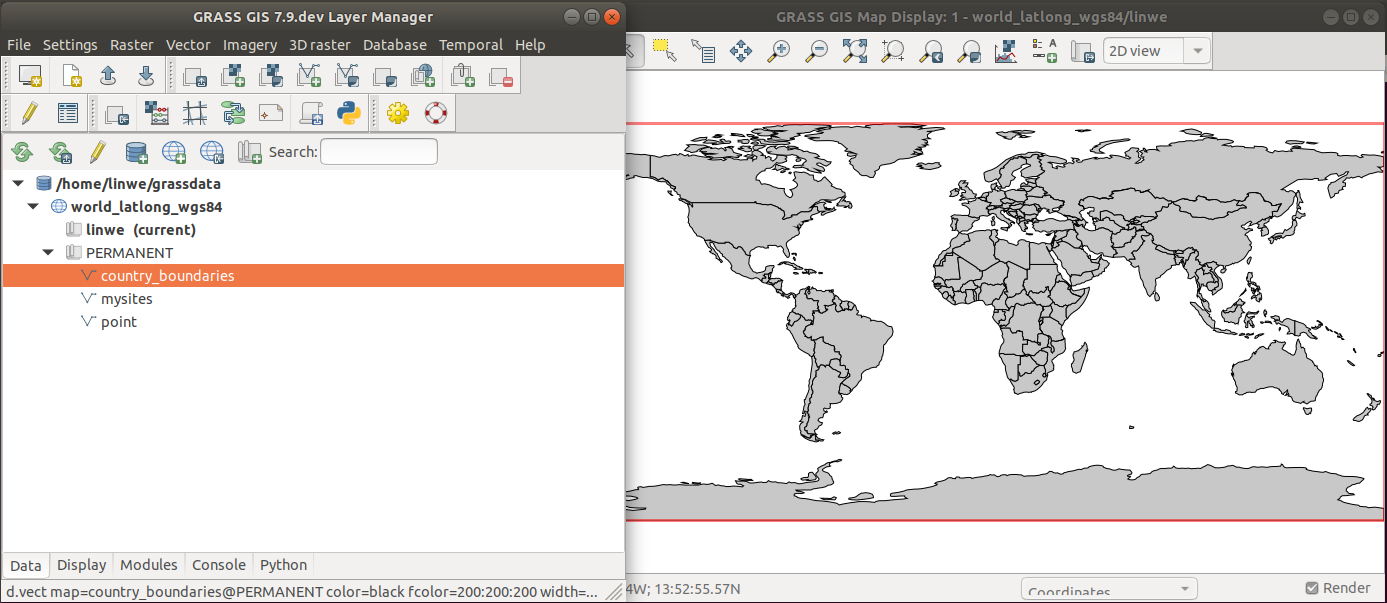
\includegraphics[width=17cm]{../pictures/demolocation.png} 
\caption[World map as a part of the default location]{World map as a part of the default location (Source: Personal collection)}
\label{fig:demolocation}
\end{center}
\end{figure}

\noindent \textbf {Various options for starting GRASS GIS}

\large \noindent In addition to the software components that the user
encounters during startup and to the state that the software finds
itself immediately after startup, the startup mechanism also includes
the way how GRASS GIS can be started. Because users of this software usually
work under a Unix operating system, GRASS is usually run from the
command line. 

\vspace{0.3cm}
\begin{figure}[hbt!] 
\begin{center}
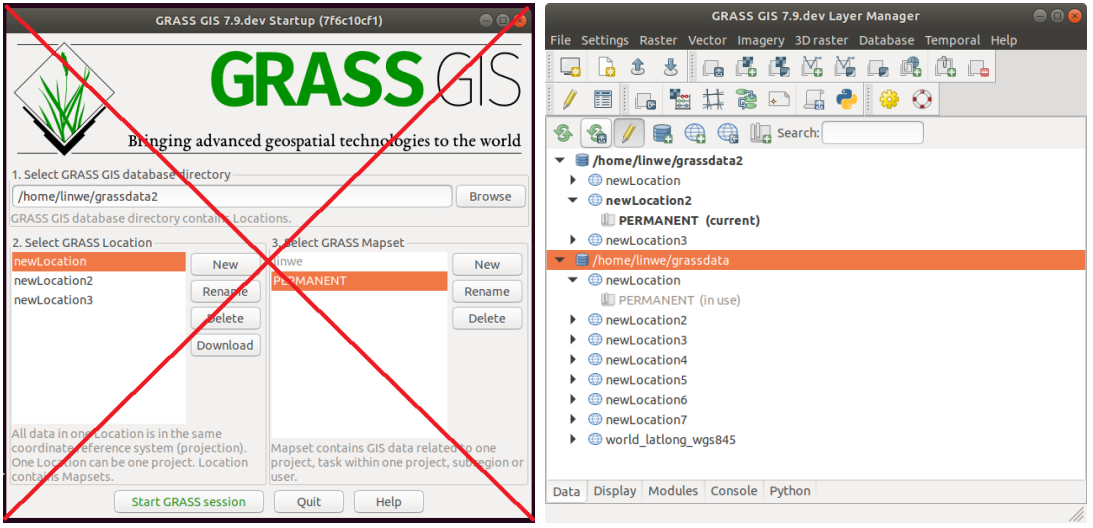
\includegraphics[width=17cm]{../pictures/last_mapset_startup.png} 
\caption[GRASS starts in the last used mapset]{GRASS starts in the last used mapset (Source: Personal collection)}
\label{fig:last_mapset_startup}
\end{center}
\end{figure}

\noindent Advanced users often do not even run the graphical
environment and perform all geographic analyzes using the command
line. This is also why the command line window runs in the background
throughout the work with this software. In the thesis, however, the author
mainly focuses on first-time users.
% ML: "we" is heavily used in this thesis, here it's not clear what
% mean "we", try to rewrite the sentence
% LK: changed to ''author''
The software can be run from 
the command line in the following way \cite{startup}:

\noindent \texttt{:$\sim$\$ grass79} \\
\noindent Start GRASS using the default user interface. In version
7.8, the user is prompted by the startup screen. 
Appropriate location and mapset must be either set by command line argument
using the \texttt{:$\sim$\$ grass79
  \$HOME/grassdata/location/mapset}, or by environment variables, 
  or taken from the last
GRASS session, specifically from a file in the path
\textit{\$HOME/.grass7/rc}. 
After GSoC the startup
screen appears only when the mapset is not in the usable state.

\noindent User interface can be futher specified by Flags:

\noindent \texttt{:$\sim$\$ grass79 --gui}\\
\noindent Start GRASS using the graphical user interface.  In version
7.8, the user is prompted by the startup screen. After GSoC the startup
screen appears only when the mapset is not in the usable state.

\noindent \texttt{:$\sim$\$ grass79 --text} \\
\noindent Start GRASS using the text-based user interface and do not show the startup
screen.
%Appropriate
%% ML: location/mapset can be defined also by the argument
%% ML: grass79 --text /path/to/location/mapset
%location and mapset must be either set by environmental variables 
%by running a specific
%% ML: same usage as for --text
%mapset using the \texttt{:$\sim$\$ grass79
%  \$HOME/grassdata/location/mapset} command, or taken from the last
%GRASS session, specifically from a file in the path
%\textit{\$HOME/.grass7/rc}.
%% LK: included here
It is also possible to use
\texttt{:$\sim$\$ grass79\$ --text /path/to/location/mapset} command.

\newpage
\noindent \texttt{:$\sim$\$ grass79 --gtext} \\
\noindent Start GRASS using the text-based user interface and show startup screen.  
As it is planned to completely remove the old startup screen, in version 7.9 after GSoC, 
the new function of the \texttt{--gtext} is not defined yet. 

% ML: same usage as for --text

The possibilities of starting GRASS GIS can be further extended by the
% ML: twice "version" in a single sentence (the later can be removed)
concept of \textit{workspaces} which enables to save the current software settings
and then open it, as we can see in Figure \ref
{fig:workspace_grass}. However, the option to start a specific
workspace from the command line or to start GRASS GIS from a File
Manager using the file association of the workspace file (.gxw)
is missing.

\vspace{0.3cm}
\begin{figure}[hbt!] 
\begin{center}
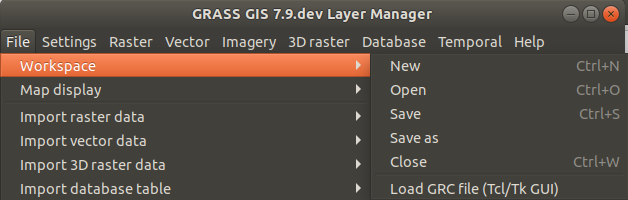
\includegraphics[width=13cm]{../pictures/workspace_grass.png} 
\caption[Management of workspaces in Layer Manager]{Management of workspaces in Layer Manager (Source: Personal collection)}
\label{fig:workspace_grass}
\end{center}
\end{figure}

\newpage
\vspace*{-1cm}
\subsection{Thesis objectives}
\label{sec:objectives}

The aim of the master thesis is to evaluate the changes made in the
% ML: find better word than "final" (nothing is final ;-)
GSoC using questionnaires, propose the suitable solution for the GRASS GIS
startup mechanism, and extend the startup mechanism by proposing 
and implementing a new solution of special mode for first-time users.
There are two fundamental questions related to the mentioned proposals,
which we will try to answer in the work:

\begin{enumerate}

\item  \noindent \textbf{How to enhance the first-time user experience?}

  \noindent As already mentioned, data hierarchy in GRASS GIS can
  cause significant problems for newcomers. Therefore, the aim of this
  work is to propose a solution on how to enhance the first-time
  user experience (see subsection \ref{sec:proposal1}) and implement
  it.


\item \noindent \textbf{How to improve the GRASS GIS startup mechanism?}

  As mentioned in the previous subchapter, in the special situation
  where the last opened mapset is not in the usable state, the ``old''
  startup screen still appears. This situation is rather a lack of a
  new solution introduced after GSoC. The important goal of this
  work is to propose a solution for how this shortcoming could be
  remedied (see subsection \ref{sec:proposal2}).

\end{enumerate}

\noindent Already during GSoC, it was decided that some form of
special mode for new users will need to be implemented. At the same
time, however, some questions remained unanswered regarding the
general startup mechanism and further direction of the GRASS GUI.

Therefore, Survey 1 Part 1 entitled \textbf {Help
improve GRASS GIS startup mechanism and Data Catalog}, see Appendix
\ref{appendix:A}, does not deal only with the second key question;
it is much broader. The goals are also to determine the level of user
satisfaction/dissatisfaction with the new solution and obtain
general user preferences regarding further improvements of the GRASS
GUI.

As it was not clear how to grab the new special mode for first-time
users, the first survey was extended by a second thematically
different section called \textbf{Help create a better first-time user
experience in GRASS GIS}, see Appendix \ref{appendix:B}. The answers
in this part of the survey are essential for deciding
of what information the special mode for first-time users should
contain and which implementation form to choose.

The aim of the second survey called \textbf{Help improve the special
mode for first-time users} is to find out whether users like the
proposed mockups of the infobar and give them space to share their 
ideas so that the implemented solution in this work is the best
possible from an objective point of view (see Appendix
\ref{appendix:C}). Both Survey 1 Part 2 and Survey 2
deal with the first question, which prevails
since all the performed implementations are based on it.

%% -------<<< Chapter 2: Enhancing the first-time user experience in other software >>>-------\\%%%%%%%%%%%%%%%%%%%%%%%%%%%%%%%%%%%%
\newpage
\vspace*{-1cm}
\fancyhead[RE, RO]{\fancyplain{}{\small \sl{Enhancing the first-time user experience}}}
\section{Enhancing the first-time user experience}
\label{subsection:enhancing}

Firstly, we need to define what we mean by the \textit{first-time user
experience}. As \cite{ftue} states ``In human-computer interaction
and UI design, a first-time user experience (FTUE) refers to the
initial stages of using a piece of software. It commonly includes
configuration steps, such as signing up for an account. Every user of
a service has his/her FTUE, even if he/she has extensive experience
with using a similar product. Patience, time investment, and
intuitiveness are factors for a user's FTUE. Software services
generally have different layouts, styles, graphics, and hotkeys which
must be identified to contribute to a user's learning, mastery, and
efficiency of the software.''

Many articles are dealing with both improving the first-time user
experience and evaluating it. For instance, \cite{BARNETT201882} deals
with the use of FTUE embedded in games on mobile devices. It implies
that FTUE has the power to affect user perception in elements of
usability -- an integral part of software development and talking
about maximizing the effectiveness, efficiency, and satisfaction of
the user. From a game design perspective, FTUE is
impactful. Similarly, \cite{smartphones} investigates the experience
of users who use new gesture control features of smartphones and
tablets for the first time. The study reveals the advantages and
disadvantages of new gesture control features and based on results
suggests improvements regarding the design. Also interesting is the
work \cite{onlineexamination} which studies the first-time user
experience in a website-based exam system. As in the previous article,
the conducted survey identifies several shortcomings that may be
improved in the future.

The first-time user experience is mainly related to the initial user
steps, so it is often related to the startup mechanism. So let's look
in the following subsection at selected GIS software to examine if
they use any features that enhance the first-time user experience or
even the user experience in general. Then we move even beyond GIS and
look at some other interesting ways how to improve the first-time user
experience.

\subsection{GIS software}
\label{subsection:GIS software}

\noindent In Figures \ref{fig:hodnoceni_all} and
\ref{fig:hodnoceni_free} we can see graphs of the 10 highest rated GIS
% ML: in following text you are using "open-source" term rather than "free"
% LK: changed
software and the 10 highest rated free GIS software in 2020, as stated
in the evaluation taken by GIS Geography online journal
\cite{gisgeography}. The evaluation is performed on a point scale from
0 to 10 in four categories - \textit{cartography, analysis, editing,
  and data management} which are subsequently averaged. We must keep
in mind that this evaluation is very indicative, as each software has
different strengths. GRASS GIS takes the leading position in the
\textit{analysis} category, with a rating of 9.8 out of 10, which is
comparable to FME and ArcGIS Pro, but in other aspects, it loses
significantly.

\vspace{0.3cm}
\begin{figure}[hbt!] 
\begin{center}
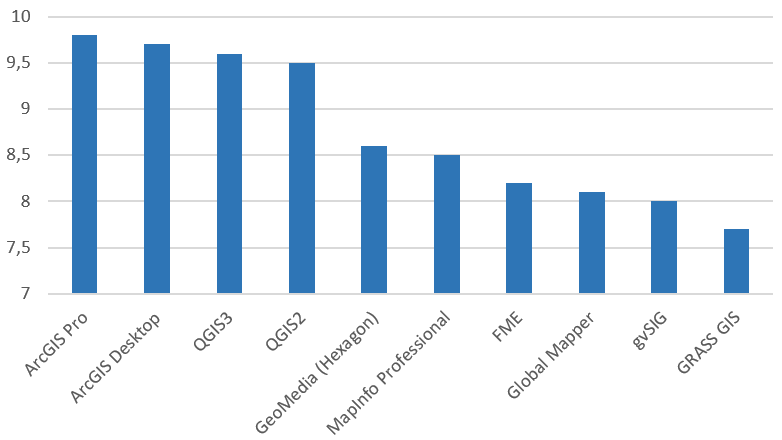
\includegraphics[width=13cm]{../pictures/hodnoceni_all.png} 
\caption[Top 10 GIS Software in 2020 according to GIS Geography journal]{Top 10 GIS Software in 2020 according to GIS Geography journal \cite{gisgeography}}
\label{fig:hodnoceni_all}
\end{center}
\end{figure}

\begin{figure}[hbt!] 
\begin{center}
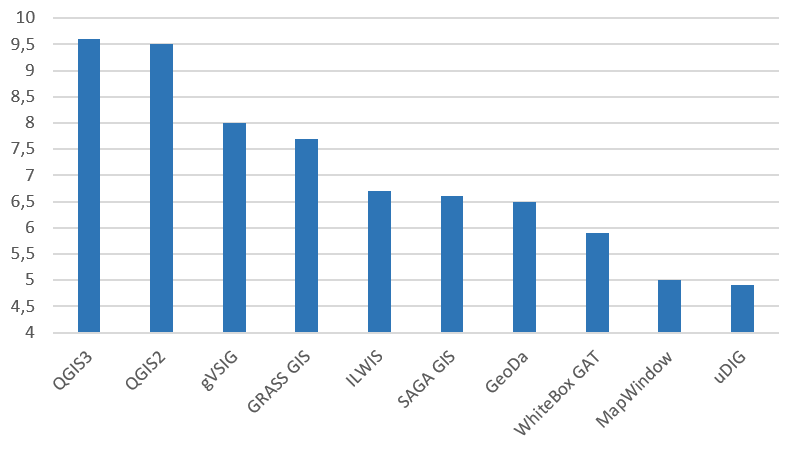
\includegraphics[width=13cm]{../pictures/hodnoceni_free.png} 
\caption[Top 10 free GIS Software in 2020 according to GIS Geography journal]{Top 10 free GIS Software in 2020 according to GIS Geography journal \cite{gisgeography}}
\label{fig:hodnoceni_free}
\end{center}
\end{figure}

\noindent For the following analysis, the three highest-rated
proprietary software were selected - ArcGIS Pro (ESRI), GeoMedia
(Hexagon), and MapInfo Professional (Pitney Bowes) as well as the four
highest-rated free software (excluding QGIS 2 and GRASS
GIS). The software is analyzed using the following three questions:

\begin{itemize}
\item What data hierarchy does the software use compared to GRASS GIS?
\item Has the software startup screen? And if so, is always displayed? How does it look like? 
\item Does the software have features for enhancing the first-time user experience, and if so, in what form?
\end{itemize}

\noindent The information obtained about proprietary GIS software is
summarized in Figure \ref{fig:proprietary_software}.

% ML: Note that in GRASS a workspace is not store in data hierarchy (by default)
% ML: ArcGIS project is probably more closed to GRASS database
% ML: You can have several GRASS workspace files for single mapset defined
% ML: Be careful with "GRASS workspace" term - what do you exactly mean by this term?
% ML: Also note that "GRASS workspace" term is not clearly explained in the text (AFAIR)
\vspace{0.3cm}
\begin{figure}[hbt!] 
\begin{center}
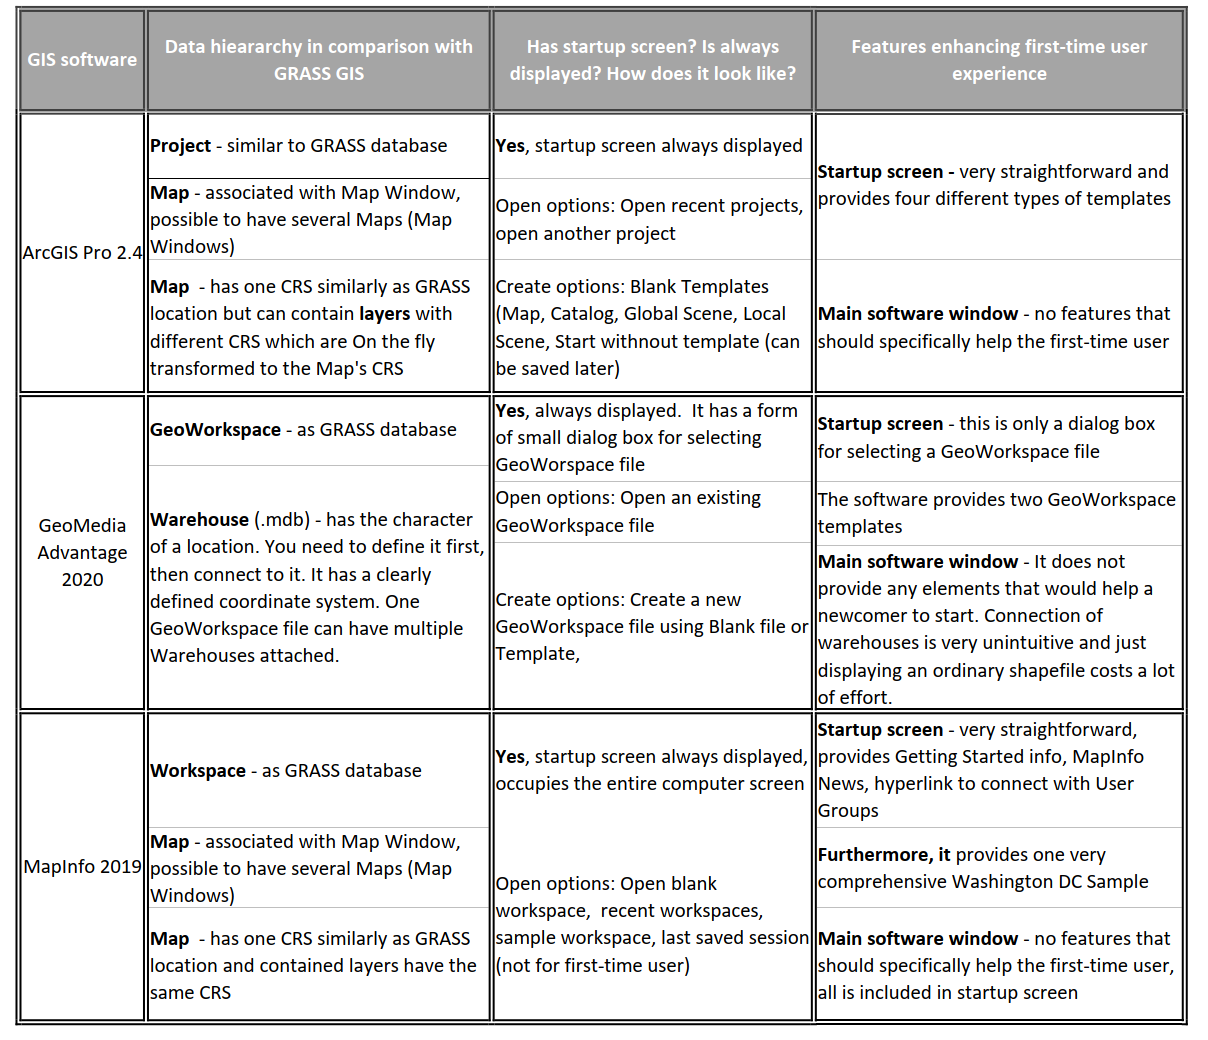
\includegraphics[width=17cm]{../pictures/proprietary_software.png}
\caption[Summary of selected proprietary software]{Summary of selected proprietary software (Source: Personal collection)}
\label{fig:proprietary_software}
\end{center}
\end{figure}

\noindent In terms of enhancing the first-time user experience, the
most interesting deeds are the startup screens of the ArcGIS Pro 2.4
and MapInfo 2019 software. The startup screen of MapInfo 2019 (see
Figure \ref{fig:map_info_startup_screen}) atypically occupies the size
% ML: skip "new" 
% LK: skipped
of the entire computer screen. It provides links to news
or links to videos on YouTube that can help first-time users. In the
upper right part of the startup screen, it is possible to run help,
which has the character of a separate desktop application. In the left
part, there is a simple bar allowing us to choose a workspace we want
to work in. We can open an empty workspace, sample workspace with a
map of Washington DC, or choose another previously saved workspace in
the directory path. If we run the software again, the Open Last Saved
Session option will be added to the startup screen.

% ML: why two tables (two headers)
% ML: why there is GRASS only after GSoC (and not before?)
\vspace{0.3cm}
\begin{figure}[hbt!] 
\begin{center}
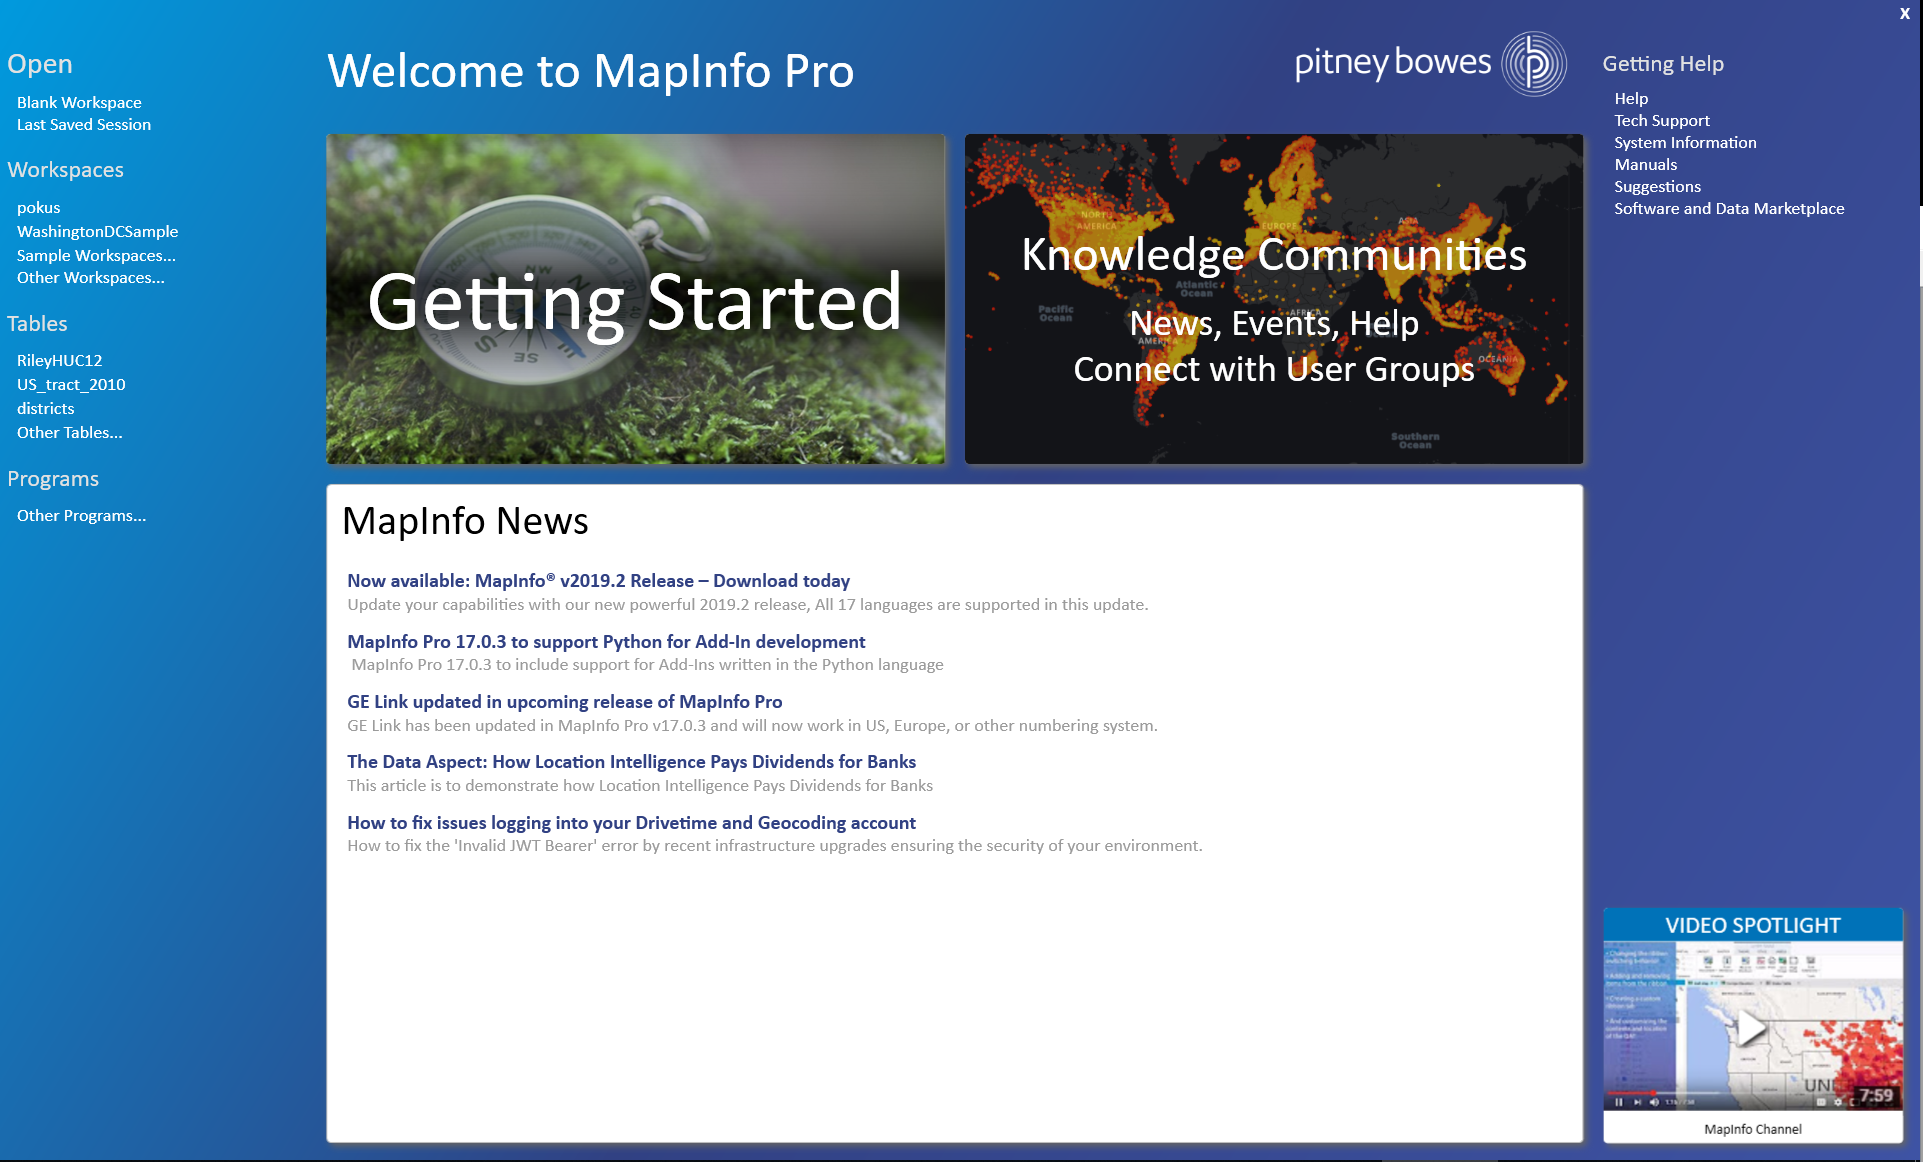
\includegraphics[width=16cm]{../pictures/map_info_startup_screen.PNG} 
\caption[MapInfo Professional 2019 startup dialog]{MapInfo Professional 2019 startup dialog (Source: Personal collection)}
\label{fig:map_info_startup_screen}
\end{center}
\end{figure}

\noindent The ArcGIS Pro 2.4 also has its startup screen. Here we can
open recently saved projects or select from pre-prepared templates
(Map (standard), Catalog, Global scene, and Local scene). Another
option is to select an empty sheet.

The information obtained about free GIS software is summarized
in Figures \ref{fig:open-source_software}, \ref{fig:grass_gis_software}. 
In terms of improving the
first-time user experience, QGIS 3 is the most interesting. After the
introduction, the user is redirected to the main software window
informing him about community events and improvements. Here the user
can choose an empty project template or open sample datasets (North
Carolina, South Dakota, Alaska) provided along with installation. QGIS
3 also shows an informative warning message (see Figure
\ref{fig:qgis_warning_window}) that appear quite often in a variety of
situations. This infobar can be helpful for new as well as experienced
QGIS users.

\vspace{0.3cm}
\begin{figure}[hbt!] 
\begin{center}

\includegraphics[width=17cm]{../pictures/qgis_warning_window.JPG} 
\caption[Informative warning message  in QGIS 3.14]{Informative warning message  in QGIS 3.14 (Source: Personal collection)}
\label{fig:qgis_warning_window}
\end{center}
\end{figure}

\vspace{0.3cm}
\begin{figure}[hbt!] 
\begin{center}
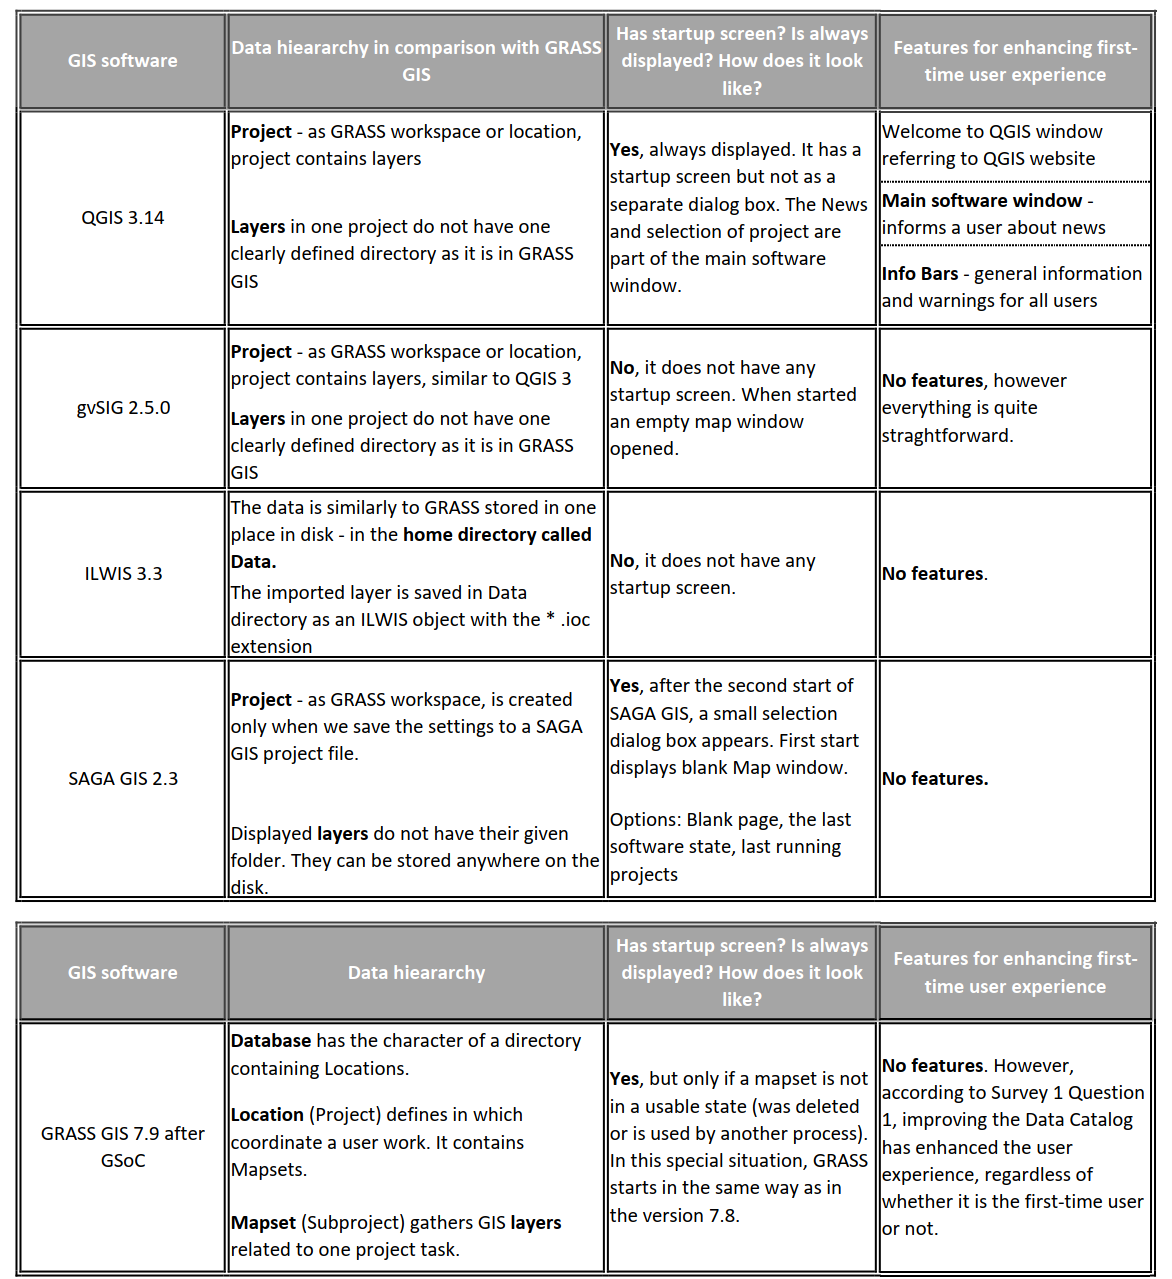
\includegraphics[width=16.5cm]{../pictures/open-source_software.png} 
\caption[Summary of selected free GIS software]{Summary of selected free GIS software (Source: Personal collection)}
\label{fig:open-source_software}
\end{center}
\end{figure}

\vspace{0.3cm}
\begin{figure}[hbt!] 
\begin{center}
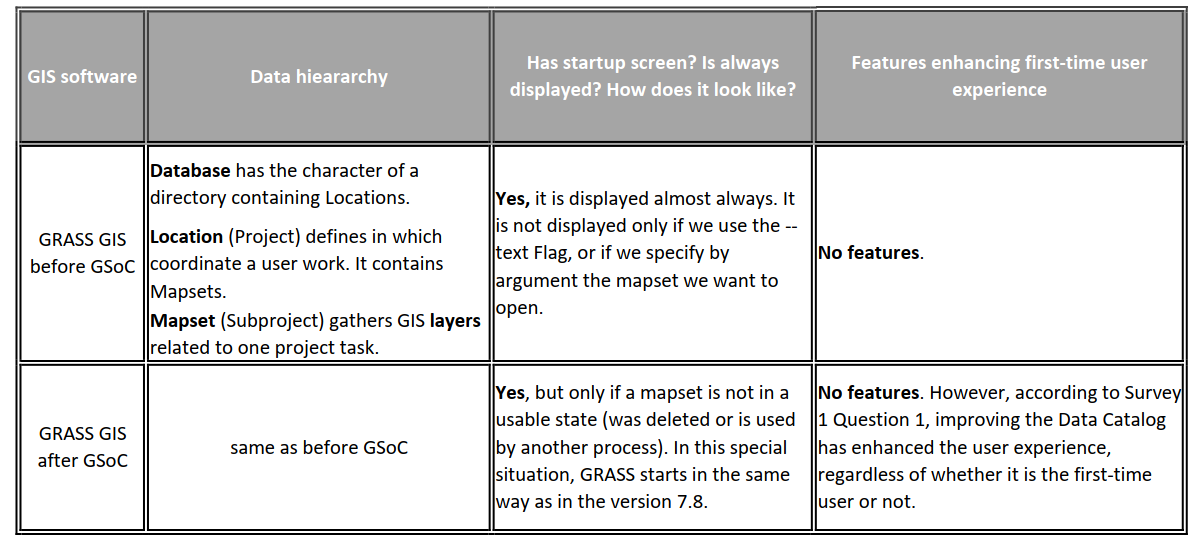
\includegraphics[width=16cm]{../pictures/grass_gis_software.png} 
\caption[Summary of GRASS GIS software]{Summary of GRASS GIS software (Source: Personal collection)}
\label{fig:grass_gis_software}
\end{center}
\end{figure}

\noindent In the cross-section of all selected GIS software, we can
notice that the data hierarchy is quite different. The truth is that
two world-famous representatives of GIS software -- ArcGIS Pro and
QGIS 3 -- have similar data organization into projects. However, in
the data hierarchy of the other two proprietary software GeoMedia and
MapInfo, the term `` project '' does not appear at all. It is
therefore good to realize that we may consider `` project '' as a
standard element of data organization, especially for free GIS
software, but after looking at proprietary software we find out that
data organization across software is surprisingly different not only
from a technical point of view but also in terms of different names.

Startup screens appear in some form in all selected
proprietary software. For GeoMedia, it is a small dialog box whose
purpose is purely organizational -- choose the GeoWorkspace you will
work in. For ArcGIS Pro and MapInfo, startup screens play a more
important role. It tries to impress users with both modern design and
the services they offer. Similarly, QGIS tries to make contact with
the user from the beginning -- it refers to news and displays info
bars.

It is surprising how much of a difference there can be between
proprietary GIS software in terms of efforts to enhance the first-time
user experience. With the GeoMedia software, the author did not manage
to record any effort at all, on the contrary, MapInfo is very generous
to its user from the very beginning and uses modern technologies in
the startup screen, such as videos on YouTube. Despite the fact that
in some of the selected software there is a certain effort to better
interact with the initial user, none of them contains any First Run
Wizard incorporated directly in the main software window (as offered
by Zoner Photo Studio X, see the next chapter
\ref{sec:other_software}). However, it may not be necessary. Whether
any help at all makes sense and is not rather counterproductive
strongly depends on the complexity of data organization in particular
software. For example, gvSIG software does not have any startup screen
or helpful explanation, although it can be assumed that the new user
will find his way around without any problems. GeoMedia also lacks any
interactive features, however, as data organization is more complex to
understand, it is likely to be a much more inconvenient start for
users.

As known, GRASS GIS went a different way from the beginning. Not only
in data organization. The difference between GRASS and other GIS
software goes far beyond the startup mechanism or data
organization. Let's remember the unique Unix philosophy, where the
software consists of a collection of small applications called
modules, or the ability to call these modules from the command
line. It is, therefore, interesting to note that the comparison of GRASS
GIS with other GIS software does not provide significant inspiration
for other implementations associated with the improvement of the
startup mechanism, which requires (and probably deserves) a completely
unique solution whose roots were laid already in the summer of 2020 by
GSoC implementations. However, the comparison offers an interesting
look at this topic, which is not talked about much, but certainly has
a big impact on the whole software. The evidence may be, after all,
user
complaints\footnote{\url{https://trac.osgeo.org/grass/ticket/3474}}
about the problematic startup mechanism in versions before GSoC.  We
do not have to look for inspiration only in GIS software. The
interaction with a first-time user is a completely general thing 
in all types of software.

\newpage
\vspace*{-1cm}
% ML: try to find better section name
\subsection{Other software}
\label{sec:other_software}

In this subsection, the author presents several interesting solutions
for the enhancement of the first-time user experience in other
software. It doesn't have to be just a first-time user
experience. Generally speaking, a good user experience means that the
user does not need a manual since everything is ready and
straightforward. The user is led through the process with the guided
tour or a combination of implicit and explicit action cues that show
the way \cite{ftue2}. The author found two interesting ways to enhance
the first-time user experience which are the inspiration for Survey 1
Part 2 Question 1 and Question 2. This work focuses on software
solutions, however, there are also mentioned several examples of web
solutions.

The first option, which is directly related to the improvement of the
first-time user experience and often replaces the startup screen, is
the First Run Wizard. It can take the form of a configuration (see
\cite{lansweeper}, \cite{jetbrains}) or explicitly educational. As
GRASS GIS has a steep learning curve, this work is mainly about the
educational form. An interesting example of an educational First Run
Wizard is offered by the Zoner Photo Studio X software. As can be seen
in Figure \ref{fig:zoner}, the guide consists of five parts.

\vspace{0.3cm}
\begin{figure}[hbt!] 
\begin{center}
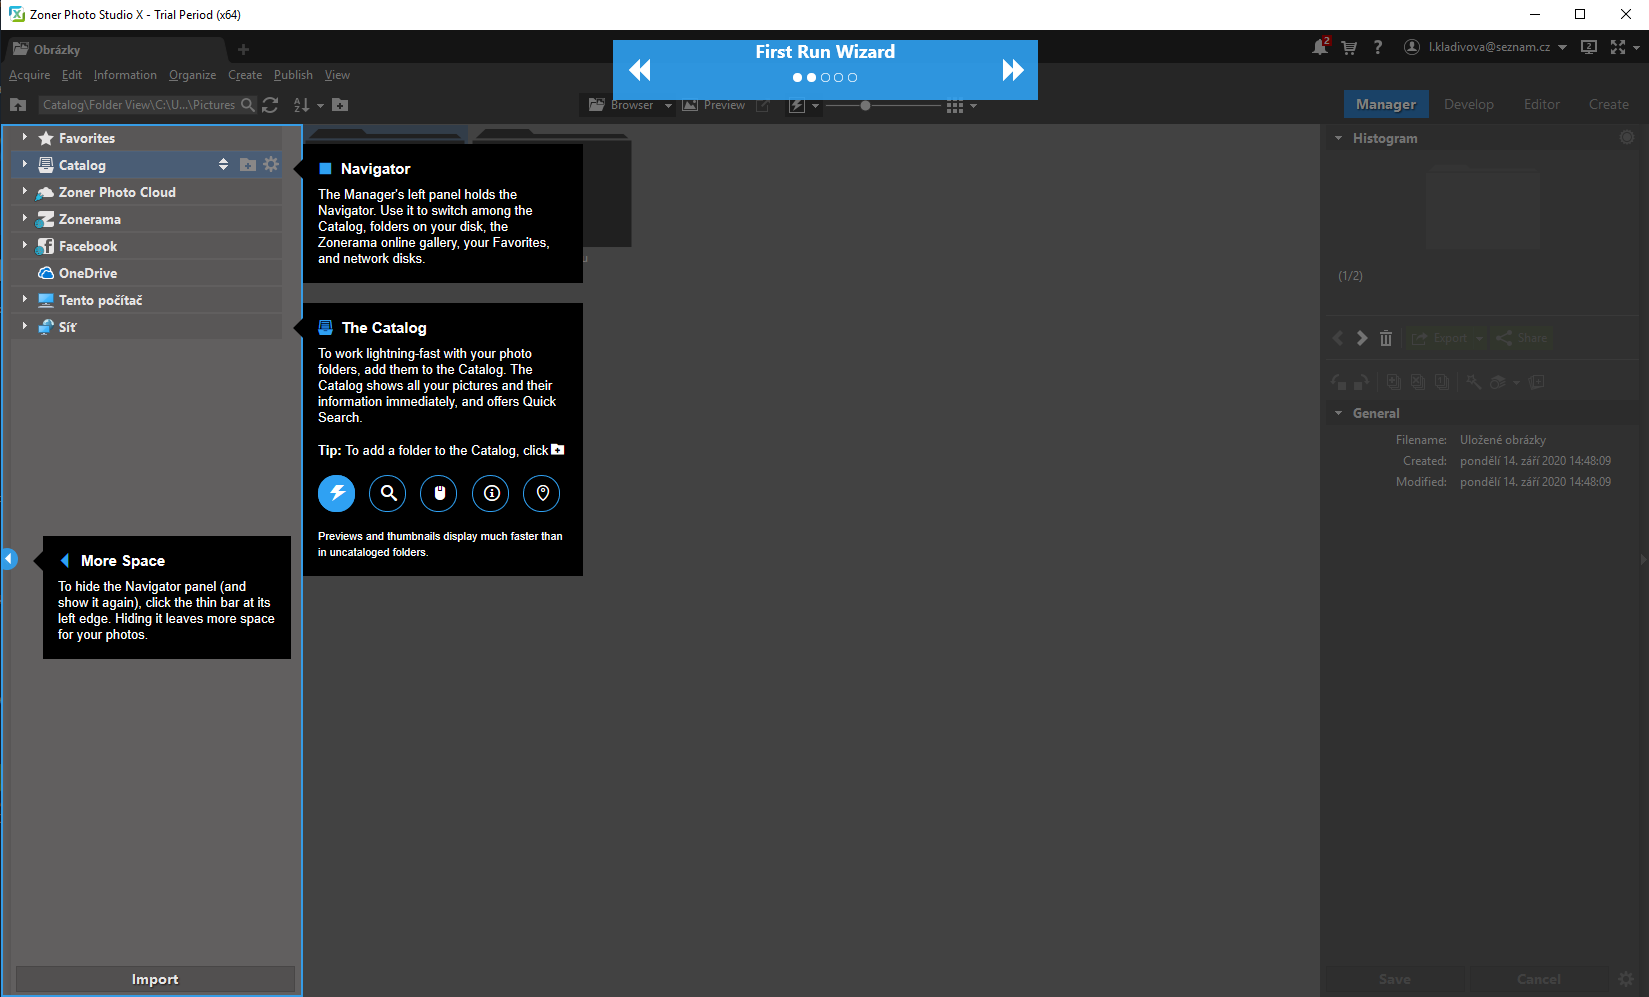
\includegraphics[width=17cm]{../pictures/zoner_first_run_2.png} 
\caption[Second page of First Run Wizard in Zoner Photo Studio X]{Second page of First Run Wizard in Zoner Photo Studio X (Source: Personal collection)}
\label{fig:zoner}
\end{center}
\end{figure}

\newpage
\noindent The first two sections introduce the software and main
tabs. The following two pages of a guide describe photo thumbnails and
zooming. The last page of the wizard lists the right toolbar and the
three individual modules -- Manager, Develop, and Editor. The main
software components described in the wizard are always marked with a
blue frame and the individual information windows are assigned to a
particular part by arrows. The wizard is not only at the beginning,
but also when using the above-mentioned modules for the first time.

The second example -- infobar -- may not only improve the first-time
user experience. It most often provides a globally visible means of
alerting users and publishing notifications. Presenting basic
information or notifications to the user may also include a button to
perform a follow-up action, as in the example in Figure
\ref{fig:info_infobar_1}.

\begin{figure}[hbt!] 
\begin{center}
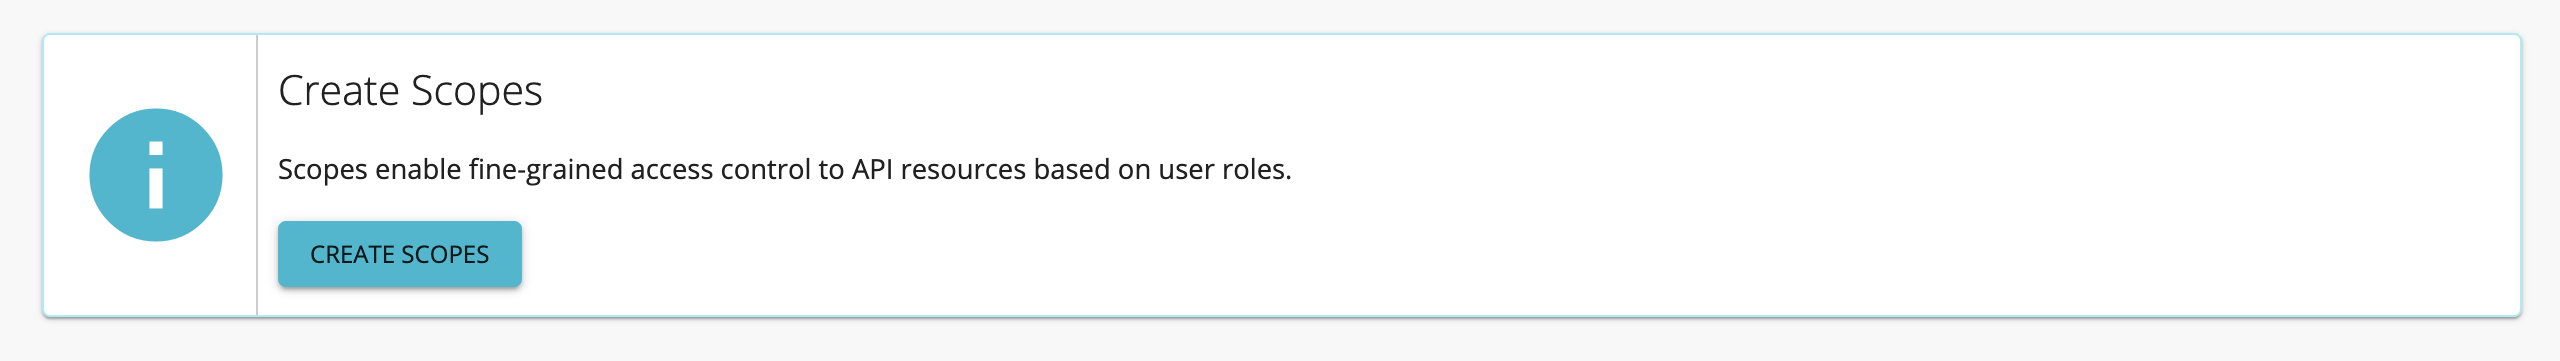
\includegraphics[width=17cm]{../pictures/info_infobar_1.png} 
\caption[Advising infobar in API Manager]{Advising infobar in API Manager (Source: \cite{githubio})}
\label{fig:info_infobar_1}
\end{center}
\end{figure}

\noindent An infobar usually enhances the general user experience. The
% ML: why exception (?)
exception is, e.g., the infobar in Matlab Simulink (see Figure
\ref{fig:info_advice_infobar}) having the character of advice for the
first-time user.

\begin{figure}[hbt!] 
\begin{center}
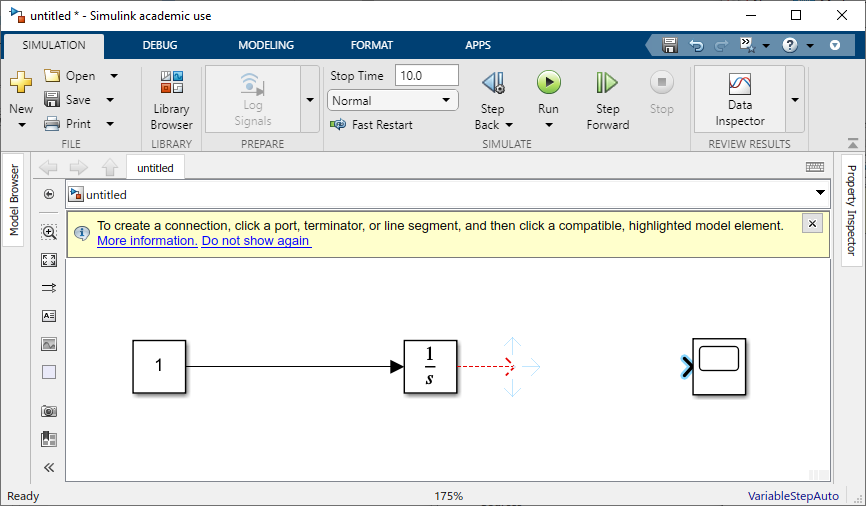
\includegraphics[width=17cm]{../pictures/info_advice_infobar.png} 
\caption[Advising infobar in Matlab Simulink]{Advising  infobar in Matlab Simulink (Source: Personal collection)}
\label{fig:info_advice_infobar}
\end{center}
\end{figure}

\noindent The topic of infobars is modern mainly in the web or
smartphone world, where a lot of interesting designs are created, some
examples can be seen in Figures \ref{fig:bootstrap_infobar} and
\ref{fig:infobar_android}.

\vspace{0.3cm}
\begin{figure}[hbt!] 
\begin{center}
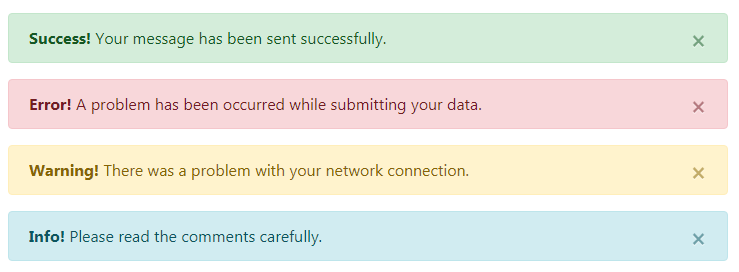
\includegraphics[width=15cm]{../pictures/bootstrap_infobar.png} 
\caption[Bootstrap alert messages]{Bootstrap alert messages (Source: \cite{bootstrap})}
\label{fig:bootstrap_infobar}
\end{center}
\end{figure}

\vspace{0.3cm}
\begin{figure}[hbt!] 
\begin{center}
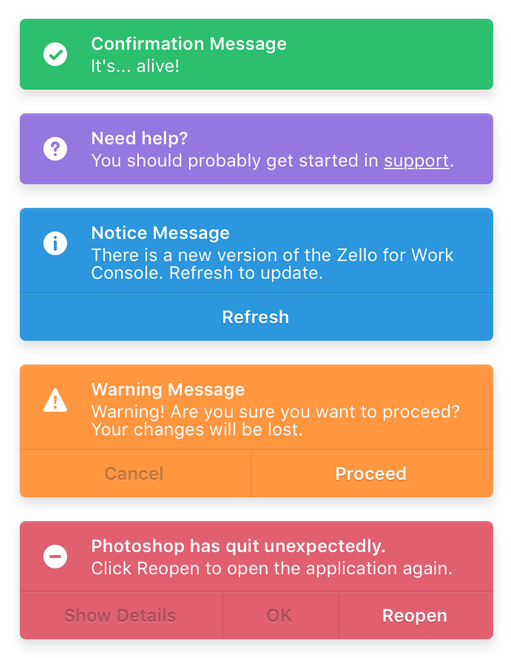
\includegraphics[width=8cm]{../pictures/infobar_android.png} 
\caption[Example of infobar design for Android]{Example of infobar design for Android (Source: \cite{pinterest})}
\label{fig:infobar_android}
\end{center}
\end{figure}

\noindent In the following chapter the author describes the
possibilities of usability testing, which is closely related to the
questionnaires -- the main decision criteria of this work.

%% -------<<< Chapter 3: Usability testing methods >>>-------\\%%%%%%%%%%%%%%%%%%%%%%%%%%%%%%%%%%%%
\newpage
\vspace*{-1cm}
\fancyhead[RE, RO]{\fancyplain{}{\small \sl{Usability testing methods}}}
\section{Usability testing methods}
\label{sec:usability_testing}

\noindent As Ana Amélia describes in her work \cite{amelia}, the
concept of usability is related to the field of
Human-Computer-Interaction (HCI). Here we can find several definitions
of what usability means. In the case of websites and software
applications, usability refers to whether or not users can achieve
specific goals with efficiency, effectiveness, and satisfaction
\cite{dishman}. As pointed out by \cite{hotjar}, the main goal of
usability testing is to test and validate the product hypothesis and
specific design decisions using the end-user perspective. We can come
across various options for dividing usability testing methods. One
possible division is nicely captured in Figure
\ref{fig:usability_testing_methods}.

\vspace{0.3cm}
\begin{figure}[hbt!] 
\begin{center}
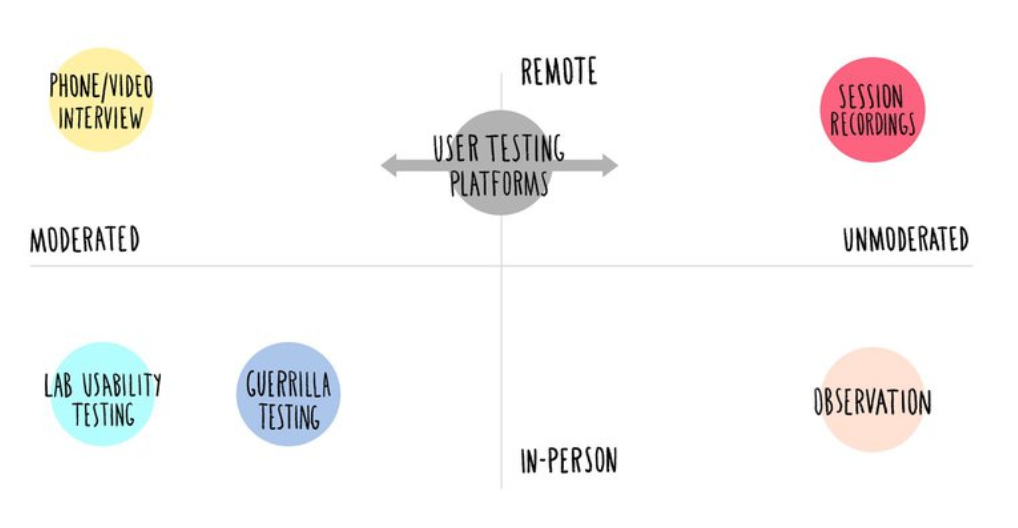
\includegraphics[width=15cm]{../pictures/usability_testing_methods.png} 
\caption[Usability testing methods]{Usability testing methods (source: \cite{hotjar})}
\label{fig:usability_testing_methods}
\end{center}
\end{figure}

\noindent \textbf {Guerrilla testing}

\noindent This is the simplest form of \textit{Moderated + in-person usability}
% ML: "test best" ? probably some word is missing?
% LK: added ``suitable for''
test suitable for the early stages of the product development process. The
people are asked to perform a quick usability test, often in exchange
for a small gift. Test subjects are chosen at random from a public
place, so that they may have no history with a product. This is the
reason why Guerrilla testing is not suitable for testing products that
require having special skills.

\bigskip

\noindent \textbf {Lab usability testing}

\noindent This type of \textit{Moderated + in-person usability} research
usually takes place inside a controlled environment that is different
from the user’s real environment. Lab usability testing works best if
we need very comprehensive and detailed information about how the user
works with the program and what problems they encounter. Participants
perform tasks and the researcher monitors them and asks questions. It
is important that the moderator is trained and able to help
participants, but at the same time, he should let them think and not
tell them exactly what to do. After testing, it is also crucial to
discuss and analyze the specific problems the participants have faced.

\bigskip

\noindent \textbf {Phone interviews and Card sorting}

\noindent In a phone usability test, a moderator verbally instructs
participants to complete tasks on their computer and collects feedback
while the user interaction is recorded remotely. This is a very good
option to test users all over the world. Card sorting is a simple
method that involves placing concepts or features on virtual cards and
allowing participants to manipulate the cards into groups and
categories. After they sort the cards, they explain their logic to a
moderator.

\bigskip

\noindent \textbf {Contextual inquiry}

\noindent Sometimes also called the Interview/Observation is the
\textit{Unmoderated + in-person} usability method suitable for
obtaining information about the user's habits and preferences or to
evaluate whether the user is satisfied with the product. A researcher
first asks a series of questions about the experience with the product
and then gives the user a task to work on independently. A researcher
will not provide any opinions and can only interfere if the
participant gets stuck on something. Otherwise, an observer remains
silent, focuses mainly on the emotions and behavior of the user, and
writes notes which will be then summarized in a detailed test report.

\bigskip

\noindent \textbf {Eye-tracking}

\noindent This special method allows scientists to observe the
movements of the user's eyes using a special device located on the
monitor, and to create heatmaps (where the user most often
looked). Eye-tracking requires a lab with special equipment and
software.

\bigskip

\noindent \textbf {Unmoderated + remote usability testing methods}

\noindent Test participants are asked to complete tasks alone in their
environment using their own devices. It does lead to the natural
participant's behavior, however, this type of testing is less
detailed. The main point is that a researcher needs to ensure that
every test instruction is clear. Unclear tasks can cause results that
miss the right objectives. It is not recommended to be used as a first
usability testing method since it does not go deep into the user’s
thinking. The most commonly used online testing tools are a 5-second
test and unmoderated card sorting. In the 5-second test, participants
have five seconds to look at a screenshot of the page before they
answer the question. Card sorting, described above, can also be
conducted in an unmoderated and remote manner if a researcher leaves
out the opportunity for follow-up questions.

% ML: there is no conclusion related to the thesis, how findings were
% used? - is it explain in other chapters, if so (including
% references), it's fine
%
% ML (updated): there is clear relation to chapter 4 (ignore comment
% above)

%% -------<<< Chapter 4: Questionnaires >>>-------\\%%%%%%%%%%%%%%%%%%%%%%%%%%%%%%%%%%%%
\newpage
\vspace*{-1cm}
\fancyhead[RE, RO]{\fancyplain{}{\small \sl{Questionnaires}}}
\section{Questionnaires}
\label{sec:questionnaires}

\noindent As the reader of this work probably realized surveys
(questionnaires) were not mentioned among unmoderated + remote
usability testing. The reason is that questionnaires are not usually
considered as usability testing because it does not require to
directly test product functionality. However, in some literature
\cite{amelia} \cite{sixusability}, questionnaires are also included in
usability testing methods. In Ana Amélia's work \cite{amelia}, for
example, the survey includes both - interview and questionnaire
techniques. The questionnaire refers to a technique that can fall
under the so-called expert/heuristic method, which works with
% ML: "a less" -> "and less" (?)
% LK: seems good
experienced people who identify problems a less experienced user might
encounter. As the author of \cite{sixusability} writes, questionnaires
are not as numerically grounded and precise as other forms or testing,
but they can provide important feedback from the user group in a short
time. They can take the form of specific questions about the software
and its future development.

Questionnaires must, above all, be effective. Therefore, in this new
field very different from the field of programming, it was necessary
to acquire new knowledge that will help avoid beginner's mistakes. How
the surveys were conceived and what they would look like eventually
crystallized by combining two different information flows.

The first flow is based on what type of questionnaire is usually used
if we want to examine the software usability. For this purpose, we can
use the widely used standard questionnaire known as the System
Usability Scale (SUS). This questionnaire having 10 five-point items
with alternating positive or negative tone was introduced by Brooke in
1996 \cite{sus}. The standard version is shown in Figure
\ref{fig:sus}. The aim of this work is to obtain more detailed
responses from GRASS users related to a specific topic, so using this
questionnaire alone does not make much sense in this work. However,
the Slider questions (see \ref{sec:slider}) are technically realized
similarly as questions in SUS - the interviewer does not evaluate
questions but statements. It can often happen that the user would not
use the queried functionality, but they assume that the others do,
which results in a positive answer. Statements encourage the user to
% ML: user vs their
% LK yes, it is strange but I think that ``their'' can be also used in some singular cases
better express their own opinions.

The second source that inspired the author in composing the
questionnaires was a user survey workshop within the All Things Open
platform in which the author participated. The visited video
conference\footnote{\url{https://2020.allthingsopen.org/sessions/user-experience-secrets-to-better-surveys-happier-users/}}
led by professionals Dan Zola and Kerry Thompson from SWAY UX set out
a few key rules for creating a questionnaire. According to the
lecturers, the questionnaire helps with the evaluation of customer
satisfaction as well as understanding who are users and what are their
pain points and priorities. It may be conducted not only at the start
of the new project but basically, at any time the survey administrator
(developer) needs user input.

\vspace{0.3cm}
\begin{figure}[hbt!] 
\begin{center}
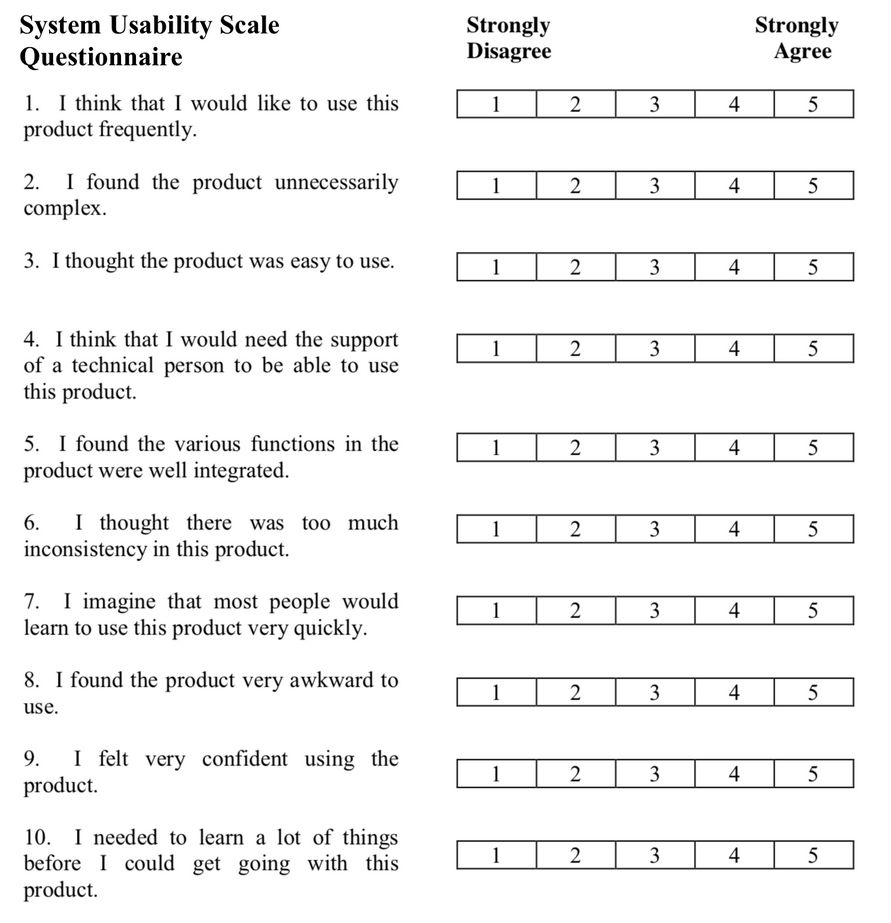
\includegraphics[width=14cm]{../pictures/sus.png} 
\caption[System Usability Scale Questionnaire (SUS) ]{System Usability Scale Questionnaire (SUS) (Source: \cite{sus})}
\label{fig:sus}
\end{center}
\end{figure}

\newpage
\noindent In order to understand what makes up a good questionnaire,
it is first necessary to clarify what constitutes a bad
questionnaire. The workshop summarized the following 8 errors in
particular:

\begin{itemize}
\item Too many questions (max 10 questions)
\item Convoluted questions
\item Answer choices that do not correspond with user's reasoning
\item Question that requires long and comprehensive answers (if open-ended questions, always put them at the beginning)
\item Answers that could have more than one meaning
\item Answers that do not provide any information
\item Straight line answers
\item Vague answers (scale from 1-10, where an answer is 5)
\end{itemize}

\noindent The latter vague answers can occur in the case of answers
with a rating scale. Although the authors of the workshop do not
explicitly mention the SUS questionnaire, they strongly recommend
avoiding the rating scale. The result could look similar to the
following example in Figure \ref{fig:blur_scale}. It is much more
advantageous to use either binary answers (Yes / No) or rank specific
features.

\vspace{0.3cm}
\begin{figure}[hbt!] 
\begin{center}
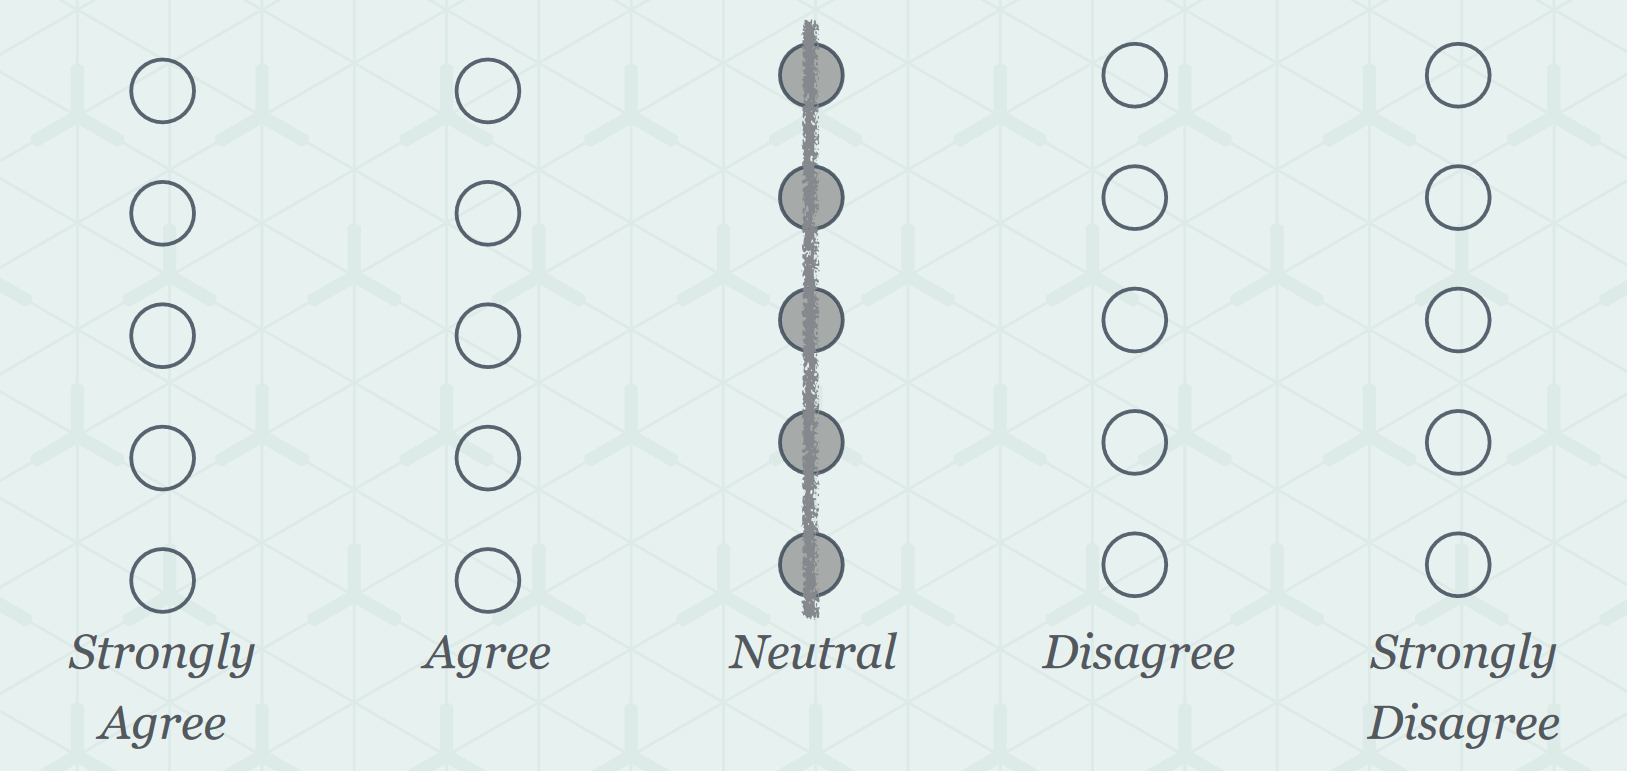
\includegraphics[width=12.5cm]{../pictures/blur_scale.png} 
\caption[Difficult interpretation of the rating scale answers]{Difficult interpretation of the rating scale answers (source: danzolakerrythompson)}
\label{fig:blur_scale}
\end{center}
\end{figure}

\noindent As mentioned at the beginning of the chapter, questionnaires
are not usually considered as usability testing because it does not
require to test product functionality. However, it would be very
challenging (if not impossible) in our work to ensure users having
both versions of GRASS GIS (version 7.8 and version 7.9 after GSoC)
and perform usability testing in the form of Lab usability testing or
Contextual inquiry methods (see section \ref{sec:usability_testing}). 
\textbf{Therefore, it was finally decided
  to use questionnaires as the main testing method.}

\subsection{Types of questions}

\noindent The author followed the advice to avoid rating scale
questions. Instead, she used Slider and Ranking methods, which
unfortunately are not offered by the free Google Forms service but
only by the paid Survey Monkey (SM) service that was eventually
used. The complete list of question types offered by the Survey Monkey
platform can be seen in Figure \ref{fig:survey_monkey_options}. Those
marked in green are used in surveys in this work. The following lines
will shed light on the advantages of the types used and the procedure
of processing them.

\vspace{0.3cm}
\begin{figure}[hbt!] 
\begin{center}
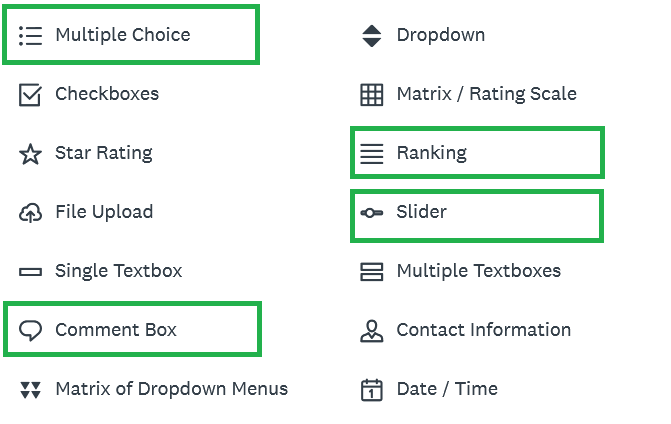
\includegraphics[width=10cm]{../pictures/survey_monkey_options.png} 
\caption[Survey Monkey question types ]{Survey Monkey question types (Source: Personal collection)}
\label{fig:survey_monkey_options}
\end{center}
\end{figure}


\noindent \textbf {Slider}
\label{sec:slider}

\noindent This type of question, also called Visual Analog Scale
(VAS), can be used instead of a rating scale. We let respondents rate
an item or statement on a numerical scale by dragging an interactive
slider. This method is visually more pleasant than the so-called
Likert scale, which is the scale used in SUS. Besides, it best
captures the true opinion and perception of users, as there is no
limited LS 'discrete set of predetermined responses. Sliders are, for
example, widely used by healthcare professionals to determine their
patient's pain. The pain does not have discrete jumps, but it is
continuous, so it is appropriate to express it on a continuous scale
from 0 to 100. As Matevž Pesek, Alja Isakovic \cite{inproceedings}
concluded the Slider (they call it Stripe) increases the
intuitiveness, simplicity, and speed of answering the
question. Therefore, this method is widely represented in the surveys
conducted in this work. The form of the questions is inspired by the
SUS questionnaire, in which users do not essentially evaluate the
question, but try to express a degree of agreement with the opinion. A
typical example of a Slider question can be seen in Figure
\ref{fig:slider_question}.

\vspace{0.3cm}
\begin{figure}[hbt!] 
\begin{center}
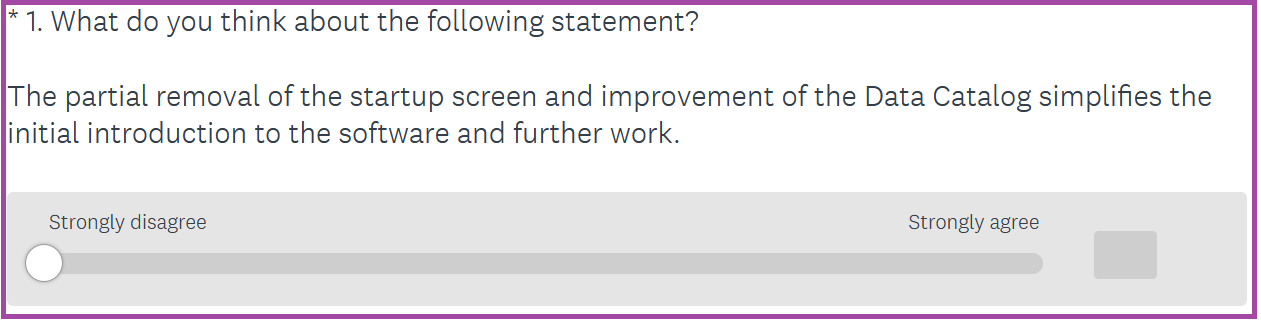
\includegraphics[width=16cm]{../pictures/slider_question.png} 
\caption[A typical example of a Slider question]{A typical example of a Slider question (Source: Personal collection)}
\label{fig:slider_question}
\end{center}
\end{figure}


\newpage
\vspace*{-1cm}
\bigskip
\noindent \textbf {Ranking}

\noindent Ranking questions require the respondent to compare items to
each other by placing them in order of preference. Although ranking
answers usually have clear answers (the result cannot be an ambiguous
answer somewhere in the middle as with the rating scale), it also has
its disadvantages. It forces respondents to decide between items that
they may perceive the same. It is also essential for this type of
question to follow the general principle that the order of the
individual options is generated randomly. Otherwise, items earlier in
the list may be more likely to be ranked highest. A typical example of
a Ranking question is provided in Figure \ref{fig:ranking_question}.

\vspace{0.3cm}
\begin{figure}[hbt!] 
\begin{center}
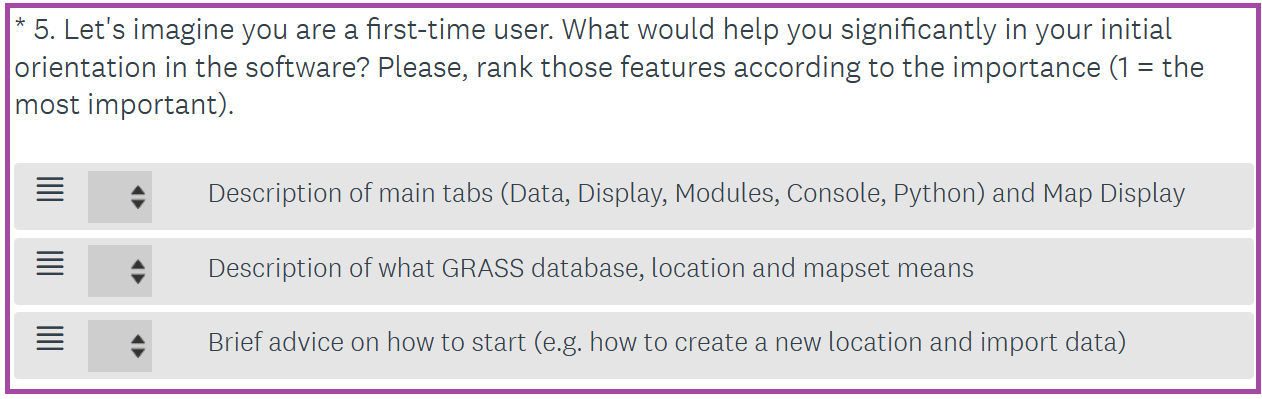
\includegraphics[width=16cm]{../pictures/ranking_question.png} 
\caption[A typical example of a Ranking question]{A typical example of a Ranking question (Source: Personal collection)}
\label{fig:ranking_question}
\end{center}
\end{figure}

\smallskip
\vspace*{-0.5cm}
\noindent \textbf {Comment Box}

\noindent This more sophisticated technique in terms of subsequent
analyzes allows the user to share their own ideas in the form of
open-ended responses. The basis of the analysis is to determine the
topics into which the answers can be categorized. It may happen that
one answer includes more topics. In this case, it is advantageous to
divide the answers into atomic parts and then categorize them. Comment
Box questions (see Figure \ref{fig:comment_box_question}) can be
further analyzed in a similar way as Multiple Choice types - by
displaying the numbers of responses in individual topics using bar
charts.

\vspace{0.3cm}
\begin{figure}[hbt!] 
\begin{center}
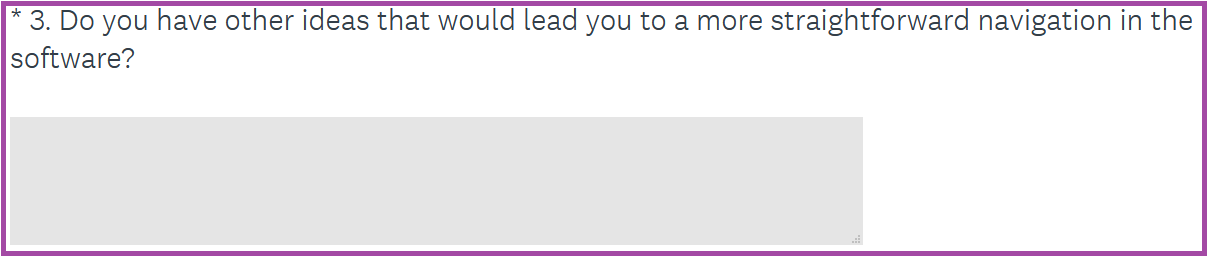
\includegraphics[width=15cm]{../pictures/comment_box_question.png} 
\caption[A typical example of a Comment Box question]{A typical example of a Comment Box question (Source: Personal collection)}
\label{fig:comment_box_question}
\end{center}
\end{figure}

\newpage
\vspace*{-1cm}
\bigskip
\noindent \textbf {Multiple Choice}

\noindent For this type of question, we also distinguish whether the
respondent can choose just one option or may check more than one. In
this work, ``One option'' variant is used (see Figure
\ref{fig:multiple_choice_question}). The disadvantage of the Multiple
Choice question is the fact that we give the respondent a fixed list
of answer options, which can skew the answers. Therefore, the ``Other
(please specify)'' variant is usually added as the last place, which
% ML: user vs their
allows the user to write their own opinion. The analysis of a question
providing the ``Other'' variant is more demanding and requires a
similar approach as the Comment Box question since it has the
character of an open-ended question. Therefore, the responses must
first be organized into topics they deal with. If many people take the
opportunity to write their own comments, it is likely that the
responses to the question were not designed correctly. Then the
assignment of open-ended responses to those originally set is more
challenging and the telling value of responses is weakened.

\vspace{0.3cm}
\begin{figure}[hbt!] 
\begin{center}
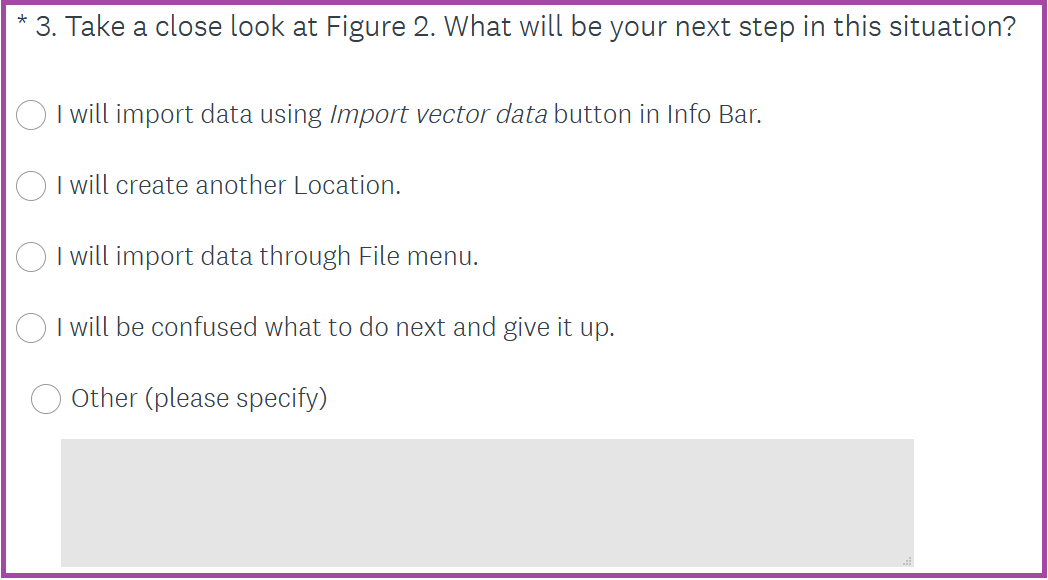
\includegraphics[width=14cm]{../pictures/multiple_choice_question.png} 
\caption[A typical example of a Multiple Choice question]{A typical example of a Multiple Choice question (Source: Personal collection)}
\label{fig:multiple_choice_question}
\end{center}
\end{figure}

\subsection{Methods of questionnaire analysis}
\label{sec:qstat}

\noindent In this work, a statistical analysis of questions is
performed, which uses the basic methods of Explanatory Data
Analysis. Thanks to this analysis, we can discover patterns or
anomalies that occur and draw the conclusions of the surveys. It is
important to understand EDA as a process that does not have given
rules, it only depends on the analyst which of the methods to use. As
this work is purely about finding out the basic features and
characteristics of a relatively small sample of answers, which counts
a maximum of 52 respondents (the number of respondents in the first
part of the first survey), we analyze data over a single
variable/column from a dataset. Therefore, we use only basic methods
such as histograms, boxplots, and probability density functions. Other
EDA tools, for example, quantile-quantile (q-q) plots, scatter plots
or correlation matrices detect relationships between two or more
variables. Descriptive statistics, which provides us with a brief
summary of the data in the sense of Mean, Standard Deviation, and 5
elements of the box-and-whisker plot (Minimum, Maximum, 25th
percentile, median, and 75th percentile), is also often considered as
a part of EDA \cite{heroku} \cite{luminousmen}. In this work Ranking
and Slider questions are analyzed using R language using RStudio. Here
the author has applied extensive experience with this program,
especially with the Tidyverse library, which is the core of data
analysis in R and itself contains several interesting packages. In
this work, the \textit{dplyr} package is used for data
manipulation. The visualization is made through the \textit{ggplot2}
\footnote{\url{https://github.com/rstudio/cheatsheets/blob/master/data-visualization-2.1.pdf}}
package. In addition to the R language, the Python language has become
the giant of data analysis with its Pandas library in recent years.

\bigskip
\noindent \textbf{Box-and-whisker plot}

\noindent This graphical method summarizes maximum and minimum values
in data, the interquartile range, and the median. It is very practical
since all of those statistics can be seen at a glance. The graphical
representation of individual parts of the graph is captured in Figure
\ref{fig:boxplot}. The central box is enclosed by two lines
corresponding to Q1 and Q3. A line (or whisker) that extends from each
edge of the box, goes to the farthest non-outlier point in the
distribution. Outliers are points that fall more than 1.5 times the
IQR from either edge of the box. Usually, they are plotted
individually.

\vspace{0.3cm}
\begin{figure}[hbt!]
\begin{center}
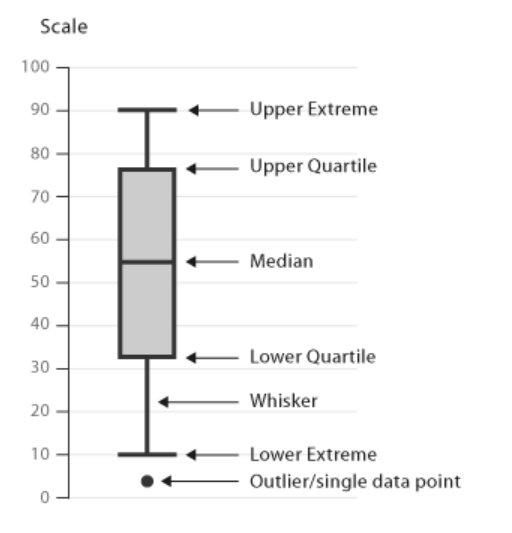
\includegraphics[width=7cm]{../pictures/boxplot.png}
\caption[Description of box-and-whisker plot (boxplot)]{Description of box-and-whisker plot (boxplot) (Source: \cite{heroku})}
\label{fig:boxplot}
\end{center}
\end{figure}

\noindent We can identify symmetry or skewness of a distribution from
a boxplot. And if more than one boxplot is plotted on the same scale,
we can visually compare the centers, the spreads, and the extreme
values of different variables.

\bigskip
\noindent \textbf {Histogram vs. Bar Chart}

\noindent A histogram is used when working with quantitative data. It
shows the number of observations that lie in-between the range of
values, which is known as a bin. Unlike a bar chart, individual
columns touch. Categorical features cannot be visualized through
histograms. Instead, we can use bar charts where elements are taken as
individual entities, so we can e.g. rearrange the blocks, from highest
to lowest \cite{OnlineMathLearning}. Illustrative comparison of
Histogram and Bar Chart is shown in the following Figure
\ref{fig:histogram_barchart}:

\vspace{0.3cm}
\begin{figure}[hbt!]
\begin{center}
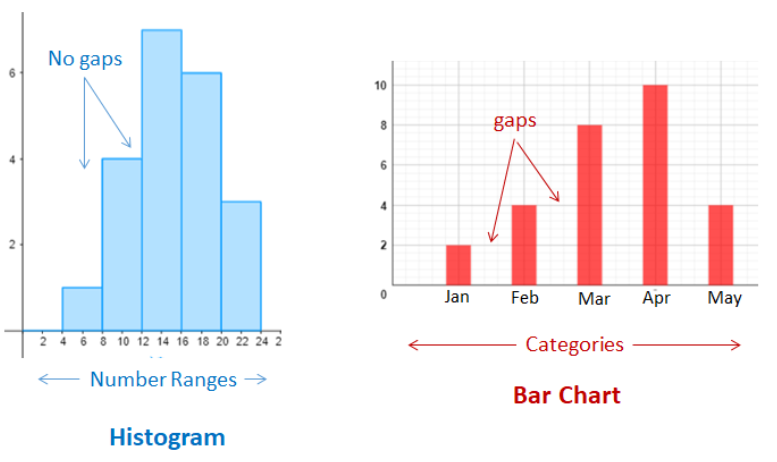
\includegraphics[width=12.5cm]{../pictures/histogram_barchart.png}
\caption[Histogram vs. Bar Chart]{Histogram vs. Bar Chart (Source: \cite{OnlineMathLearning})}
\label{fig:histogram_barchart}
\end{center}
\end{figure}

\bigskip
\noindent \textbf {Probability density function (PDF)}

\noindent Simply said the Probability density curve is the graphical
representation of the probability that a continuous random variable
falls in a particular class. Therefore, the total area under an entire
density curve is 100 \%. The probability that a continuous random
variable acquires a certain (exactly given) value is zero.

For a discrete random variable, we determine the probability that it
is equal to exactly some value. Such a function is called the
Probability mass function (PMF). It holds that all probabilities in
the function must be non-negative and together give the sum of 1.

\newpage
\vspace*{-1cm}
\subsubsection{Data types}

% ML: is the first sentence an question?
% LK: better wording made
The analysis of survey responses depends on their type. We divide two
data types - qualitative and quantitative. Qualitative data can be
further divided into binary (yes / no), nominal (contains more
categories) and ordinal (also contains more categories and can be
sorted) \cite{minitab}. For example, very hot, hot, cold, very cold,
warm are all nominal data when considered individually. But when
placed on a scale and arranged in a given order (very hot, hot, warm,
cold, very cold), they are regarded as ordinal data. Regarding
descriptive statistics, we can count and determine a mode (the most
common value in a dataset) for nominal data. Measures of central
tendency for ordinal data, in which values are ranked relative to each
other but are not measured absolutely, are limited to a mode or median
\cite{ordinaldata}.

Examples of nominal qualitative data are the responses to questions of
Multiple Choice type. Here, it is possible to create a bar chart
(where we can find the mode), but other descriptive statistics do not
make sense. An example of ordinal qualitative data is the responses to
questions of Ranking type. A bar chart can also be compiled for
Ranking questions, but the mean and standard deviation do not make
sense. Ordinal variables are not continuous variables and should not
be treated as if they are. Therefore, we should correctly create the
Probability mass function (PMF) for Ranking questions where we
determine a specific point probability on the y-axis that the discrete
random variable is equal to some order. However, in question Q3 in the
first part of the first survey and Q5 in the second part of the
survey, PDF charts were eventually used. Although their use is not
entirely correct, they provide better visual insight into the data
than PMF, especially if we have several PDF charts for different
variables.

Conversely, quantitative or numerical data can be characterized by a
numerical value. Quantitative variables can be further classified as
either discrete (those with a finite or countable number of possible
values) or continuous (those with an infinite or uncountable number of
possibilities) \cite{wisconsin1}. In the case of surveys conducted in
this work, the Slider questions always have the same form - we measure
the degree of agreement with the statement on a scale from 0 to
100. It is not a discrete variable, because we do not have any obvious
categories from the beginning. Those classes have to be created. In
this work, they were determined according to the SUS questionnaire:
[0, 20] - Strongly disagree, (20, 40] - Disagree, (40, 60] - Neutral,
(60, 80] - Agree and (80, 100] - Strongly agree.



%% -------<<< Chapter 5: Analysis of the first questionnaire>>>-------\\%%%%%%%%%%%%%%%%%%%%%%%%%%%%%%%%%%%%

\newpage
\vspace*{-1cm}
\fancyhead[RE, RO]{\fancyplain{}{\small \sl{Analysis of the first questionnaire}}}
% ML: try to find better chapter name (avoid of the of the)
\section{Analysis of the first questionnaire}
\label{sec:qstat}

\noindent The main part of this work consists of two
questionnaires. The first questionnaire was released on 23 October and
stopped on 29 October 2020. It has two separate parts. The first one
contains six questions dealing with the improvement of the GRASS GIS
startup mechanism and the assessment of the state after GSoC. The
second part of the questionnaire which is even more important for this master
thesis contains 5 questions focusing on the enhancement of the
newcomers' experience. In other words, it focuses on the possibilities of
how to enrich the existing ``demolocation'' concept so that the new
users can find their way around the software as quickly and
conveniently as possible. The implementation part of this work is
based on Survey 1 Part 2 and then especially on
the second survey, which was released roughly a month later and is
analyzed in Section \ref{sec:qstat2}.

\subsection{Part 1: GRASS startup and Data Catalog}

\noindent The first part of the survey called \textbf {Help improve
  GRASS GIS startup mechanism and Data Catalog} 
  (see Appendix \ref{appendix:A}) returns to the changes
that were implemented within the GSoC. It tries both -- to get feedback
from users and to answer questions that remain unanswered. 
From this point of view, the most fundamental question is No. 2,
which finds out the preferences regarding the way of starting GRASS
GIS in a situation where the last mapset is not in a usable
state. Questions 4, 5, and 6 are also related to the further direction
of GRASS GIS (not only in terms of the startup mechanism) while
questions 1 and 3 assess the benefits of GSoC. The first part of the
survey was attended by 52 respondents, the completion rate was high -
96 \% and no respondent skipped any questions. We can see a weekly
graph of the number of responses for a specific day in Figure
\ref{fig:survey1_part2_insight2}.

\begin{figure}[hbt!] 
\begin{center}
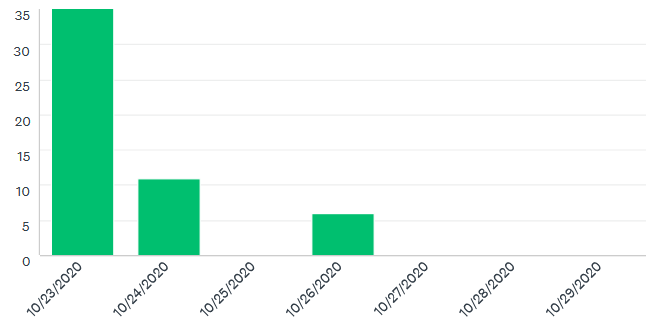
\includegraphics[width=10.5cm]{../surveys/analyzed_data/survey1_part1_insight2.png} 
\caption[Survey 1 Part 1: Responses by day]{Survey 1 Part 1: Responses by day (Source: Basic analyzes provided by the SM)}
\label{fig:survey1_part1_insight2}
\end{center}
\end{figure}

\newpage
\noindent \textbf{Question 1: What do you think about the following statement? \\
  The partial removal of the startup screen and improvement of the
  Data Catalog simplifies the initial introduction to the software and
  further work.}
\par\noindent\rule{\textwidth}{0.4pt}

\noindent This question has the form of a Slider where 0 means
complete disagreement with the statement and 100 means complete
agreement. If we only worked with an average value of 70.9, we would
conclude that enthusiasm probably prevails, but it is not so
certain. The box-whisker-plot in Figure
\ref{fig:survey1_part1_question1_boxplot} shows that the median is
significantly higher - 78.5 points out of a 100. If we look at the
histogram in Figure \ref{fig:survey1_part1_question1_histogram}, which
was divided into 5 parts exactly according to the number of bins in
the original SUS, we can see that in the last interval ``Strongly
agree'' there are 22 responses out of 52. On this basis, we can
conclude then that the vast majority like the situation after GSoC,
however, there is also a minority of negative opinions.

\begin{figure}[hbt!] 
\begin{center}
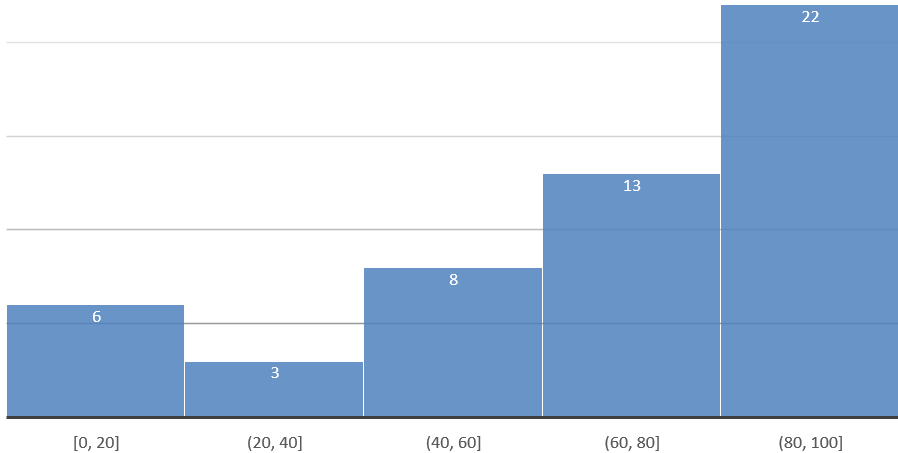
\includegraphics[width=12cm]{../surveys/analyzed_data/survey1_part1_question1_excel_histogram.png} 
\caption[Survey 1 Part 1 Question 1: Histogram]{Survey 1 Part 1 Question 1: Histogram (Source: Personal collection)}
\label{fig:survey1_part1_question1_histogram}
\end{center}
\end{figure}

\vspace{0.3cm}
\begin{figure}[hbt!] 
\begin{center}
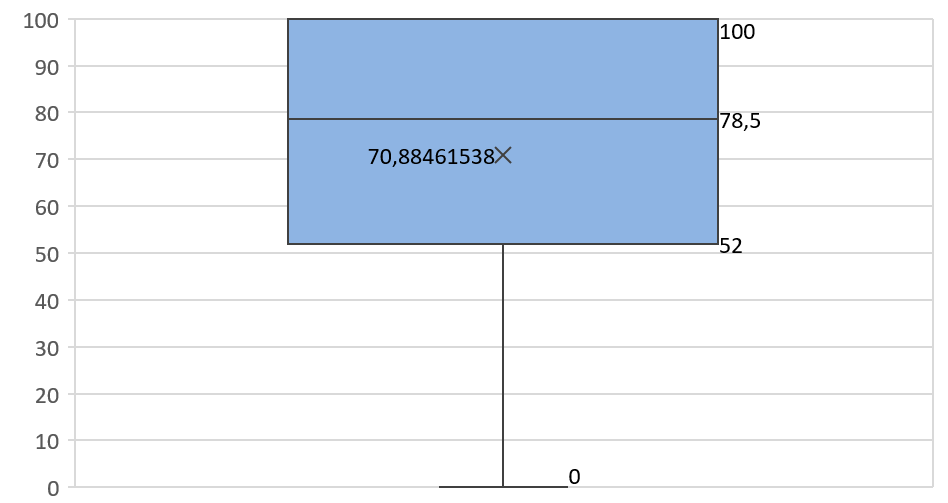
\includegraphics[width=10cm]{../surveys/analyzed_data/survey1_part1_question1_excel_boxplot.png} 
\caption[Survey 1 Part 1 Question 1: Boxplot]{Survey 1 Part 1 Question 1: Boxplot (Source: Personal collection)}
\label{fig:survey1_part1_question1_boxplot}
\end{center}
\end{figure}

\newpage
\noindent \textbf{Question 2: How do you think GRASS should start when the last mapset is not in a usable state (was deleted or is in use)?}
\par\noindent\rule{\textwidth}{0.4pt}

\noindent The result of this question put in the Multiple Choice form
with the possibility of open-ended responses is very unexpected and
unclear. Some open-ended answers strongly suggest that respondents did
not understand from the previous context to the question (see Appendix
\ref{appendix:A}, page 2) that the startup screen will not be visible
at all in other cases. Another drawback is the only two close-ended
choices. Most people, therefore, preferred something familiar (startup
screen) to the new concept of Demolocation.

One of the ways to proceed here is not to give to the result of this
question in terms of the bar chart in Figure
\ref{fig:survey1_part1_question2_histogram_sm}, as the possibilities
of answers to this question were not well-conceived, and focus mainly
on open-ended responses. Ten respondents choose neither of the two
questions offered and took the opportunity to write their own
proposal. Of the ten answers, which are categorized in the table in
Figure \ref{fig:survey1_part1_question2_other_answers}, only one
respondent \#31 is for maintaining the original startup screen. There
are some ideas of displaying a simple dialog in the form of a warning
message, which offers a user some other options -- e.g. to open a
demolocation, an existing mapset, or to create a new mapset. There was
also a suggestion that it would not be a dialog, but only a pop-up
message.

\vspace{0.3cm}
\begin{figure}[hbt!] 
\begin{center}
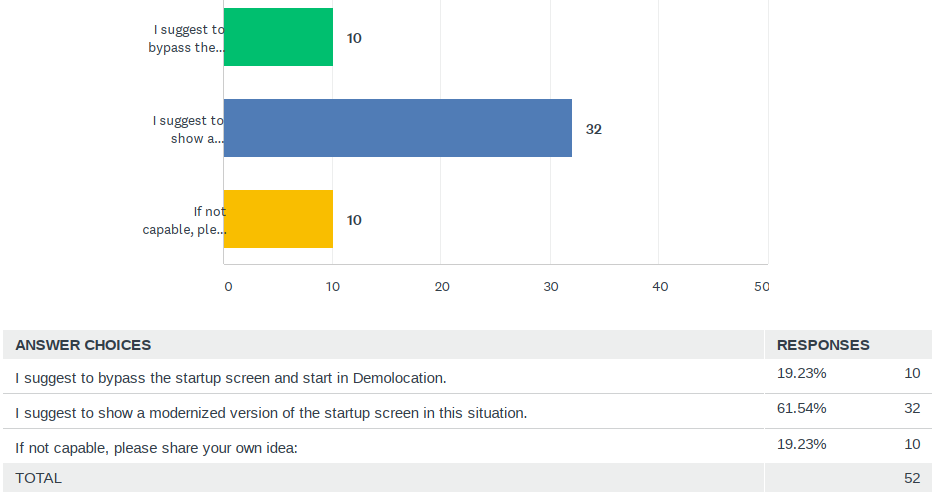
\includegraphics[width=17cm]{../surveys/analyzed_data/survey1_part1_question2_histogram_sm.png} 
\caption[Survey 1 Part 1 Question 2: Bar Chart]{Survey 1 Part 1 Question 2: Bar Chart (Source: Basic analyzes provided by the SM)}
\label{fig:survey1_part1_question2_histogram_sm}
\end{center}
\end{figure}

\vspace{0.3cm}
\begin{figure}[hbt!] 
\begin{center}
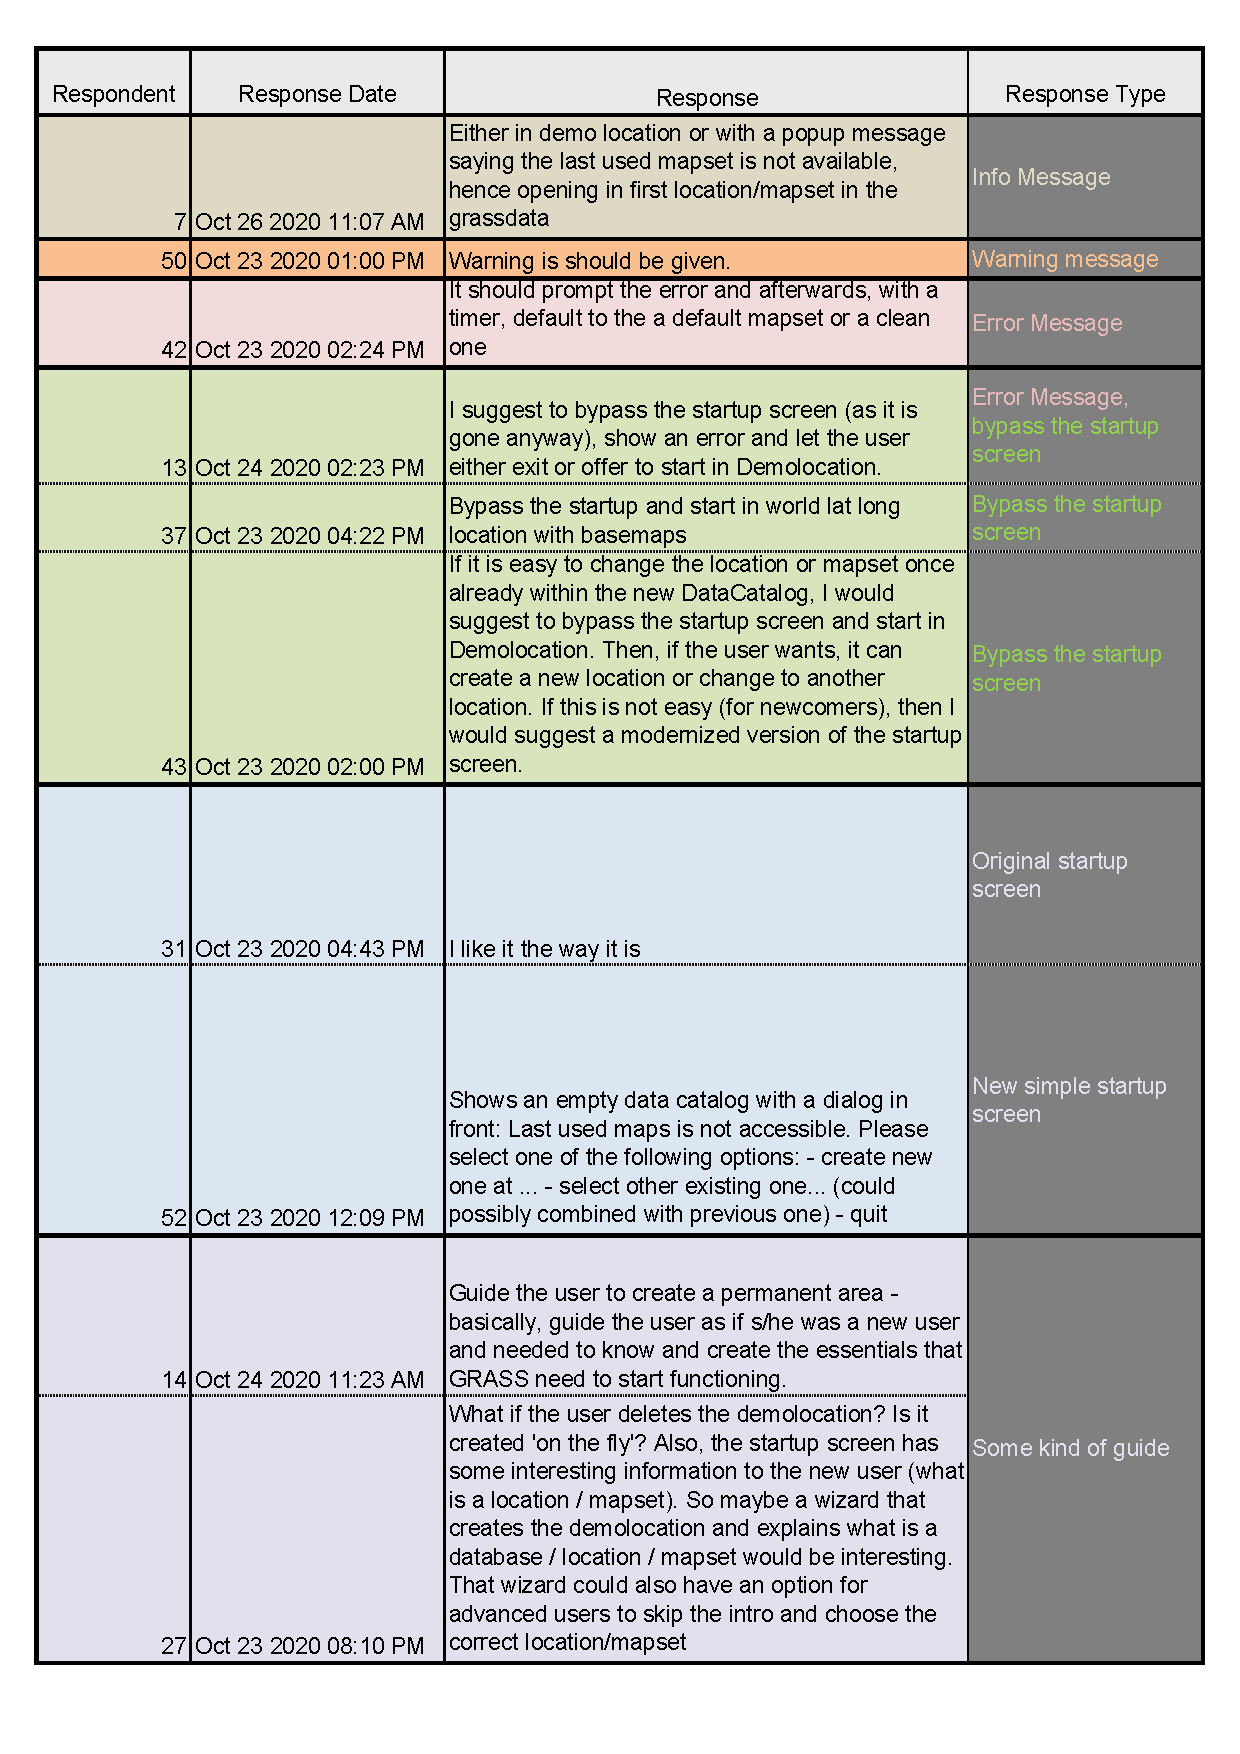
\includegraphics[width=15cm]{../surveys/analyzed_data/survey1_part1_question2_other_answers.pdf} 
\caption[Survey 1 Part 1 Question 2: Classification of open-ended responses]{Survey 1 Part 1 Question 2: Classification of open-ended responses (Source: Personal collection)}
\label{fig:survey1_part1_question2_other_answers}
\end{center}
\end{figure}

\newpage
\noindent The first option, therefore, how this case could be solved
would be to use the infobar, which would not have an informative
character (as with the proposed solution for first-time users in the
second questionnaire), but would have the character of a warning. This
Warning infobar explains why the user was redirected to Demolocation
and instructs the user to open their own project.

The second solution is to create a simple startup screen, very similar
to Moritz Lennert's Proposal
B1\footnote{\url{https://trac.osgeo.org/grass/wiki/wxGUIDevelopment/New\_Startup\#Changeparadigm}},
which explains the situation to the user (the last mapset used has
been deleted or is in use by another process) and suggests further
steps.

The advantage of changes made after GSoC is that changing the
database, location or mapset is very simple through the new Data
Catalog, as well as saving and opening workspaces. Therefore, not only
the author but also other developers are inclined rather to the
variant to completely remove any form of startup screen and employ
infobars instead.

\par\noindent\rule{\textwidth}{0.4pt} \\
\noindent \textbf{Question 3: Please, rank how useful these features in Data Catalog would be (or already are) for you (1 = the most useful).}
\par\noindent\rule{\textwidth}{0.4pt}

\noindent This question asks the GRASS user to evaluate the benefits
of the new features that were introduced after GSoC (see Figure
\ref{fig:function}) . The implementation of \textit{Small icons
  distinctive mapping, locations, GRASS databases, and layers (vector,
  raster)} is the work of Anna Petrasova, other functions are part of
the implementations performed by the author. The evaluation of
functions is performed by sorting them from the most useful (number 1)
to the least useful (number 7).

According to the means in Figure
\ref{fig:survey1_part1_question3_descriptive_stats_sm} the greatest
success have \textit{New management icons}. However, the use of mean
and standard deviation is quite misleading for ordinal types of
variables. It is better to focus on the median whose values are in
Figure \ref{fig:survey1_part1_question3_descriptive_stats_sm} marked
in a red box. The median is the smallest for \textit{Small icons
  distinguishing mapsets, locations, GRASS databases, and layers
  (vector, raster)}. Although the responses do not have the character
of a continuous random variable and the Figure
\ref{fig:survey1_part1_question3_pdf} is somewhat misleading in terms
of statistics, \textit{Small icons distinguishing mapsets, locations,
  GRASS databases, and layers (vector, raster) } are also the most
successful here. In the second place, there are \textit{New management
  icons} and in third place, we can find \textit{Creating, renaming
  and deleting mapset or location}.

Interestingly, no special success was achieved by \textit{Adding
  multiple GRASS databases}, which were relatively difficult to
implement. As can be seen from the stacked bar chart in Figure
\ref{fig:survey1_part1_question3_histogram} and also the boxplot in
Figure \ref{fig:survey1_part1_question3_boxplot_r}, the most
controversial is \textit{Mapset access info (current, in use, and a
  different user)}, which some users rated as the most useful and a
similar number of users as the least useful.

\vspace{0.3cm}
\begin{figure}[hbt!] 
\begin{center}
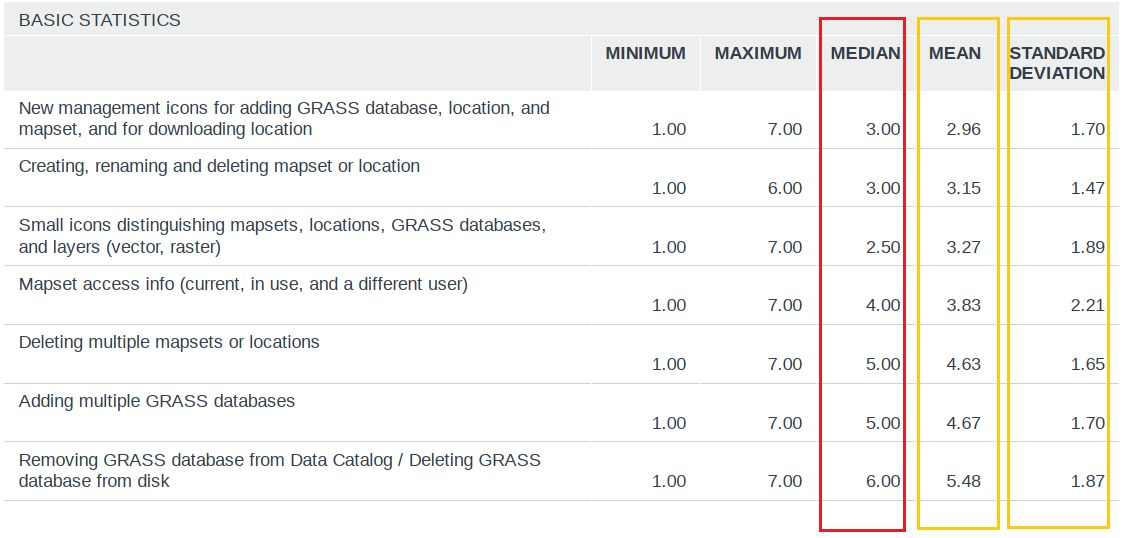
\includegraphics[width=17cm]{../surveys/analyzed_data/survey1_part1_question3_descriptive_stats_sm.png} 
\caption[Survey 1 Part 1 Question 3: Descriptive statistics]{Survey 1 Part 1 Question 3: Descriptive statistics (Source: Basic analyzes provided by the SM)}
\label{fig:survey1_part1_question3_descriptive_stats_sm}
\end{center}
\end{figure}

\vspace{0.3cm}
\begin{figure}[hbt!] 
\begin{center}
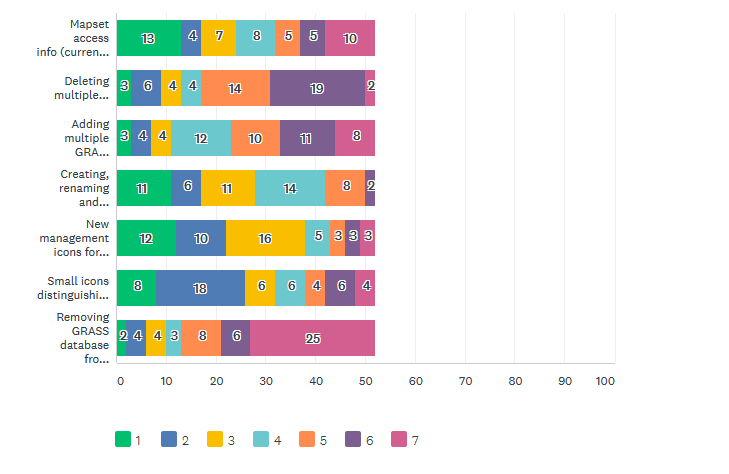
\includegraphics[width=17cm]{../surveys/analyzed_data/survey1_part1_question3_histogram.png} 
\caption[Survey 1 Part 1 Question 3: Stacked Bar Chart ]{Survey 1 Part 1 Question 3: Stacked Bar Chart (Source: Basic analyzes provided by the SM)}
\label{fig:survey1_part1_question3_histogram}
\end{center}
\end{figure}

\newpage
\vspace{0.3cm}
\begin{figure}[hbt!] 
\begin{center}
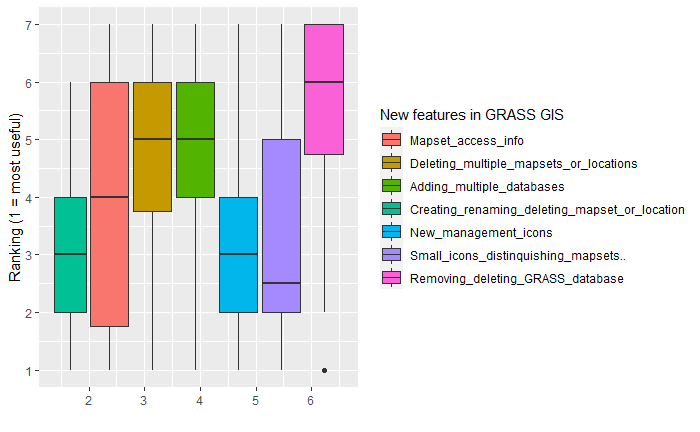
\includegraphics[width=15.5cm]{../surveys/analyzed_data/survey1_part1_question3_boxplot_r.png} 
\caption[Survey 1 Part 1 Question 3: Boxplot]{Survey 1 Part 1 Question 3: Boxplot (Source: Personal collection - R analysis)}
\label{fig:survey1_part1_question3_boxplot_r}
\end{center}
\end{figure}

\vspace{0.3cm}
\begin{figure}[hbt!] 
\begin{center}
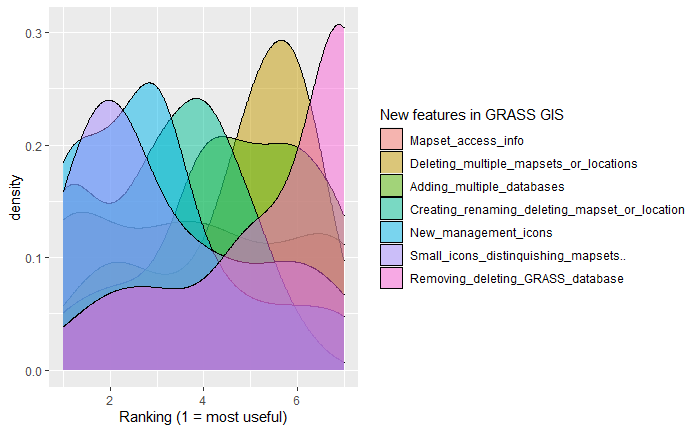
\includegraphics[width=15.5cm]{../surveys/analyzed_data/survey1_part1_question3_pdf.png} 
\caption[Survey 1 Part 1 Question 3: Probability Density Function]{Survey 1 Part 1 Question 3: Probability Density Function (Source: Personal collection - R analysis)}
\label{fig:survey1_part1_question3_pdf}
\end{center}
\end{figure}

\newpage
\noindent \textbf{Question 4: Which features would you like to add?}
\par\noindent\rule{\textwidth}{0.4pt}

\noindent From the point of view of the Data Catalog, in Figure
\ref{fig:survey1_part1_question4_open_ended}, we can see proposals for
the EPSG code shown after the location name, cloning the location,
deleting multiple layers via the context menu, displaying space-time
datasets (STDS), or displaying saved workspaces. Regarding things
unrelated to the Data Catalog, three users would like an easier and
clearer way to add WMS/WFS using a new icon.

\begin{figure}[hbt!] 
\begin{center}
\includegraphics[width=15.5cm]{../surveys/analyzed_data/survey1_part1_question4_open_ended.png} 
\caption[Survey 1 Part 1 Question 4: Classification of open-ended responses]{Survey 1 Part 1 Question 4: Classification of open-ended responses (Source: Personal collection)}
\label{fig:survey1_part1_question4_open_ended}
\end{center}
\end{figure}

\newpage
\noindent \textbf{Question 5: Because we have limited screen space, we need to think about where we can add new features.Where would you add them?}
\par\noindent\rule{\textwidth}{0.4pt}

\noindent In this Multiple Choice question analyzed in Figure
\ref{fig:survey1_part1_question5_descriptive_stats_sm} using the bar
chart, most respondents agree to add additional functions to the
context menu. Interestingly, 13.5 \% of respondents think that
\textit{no additional features should be added, there is little space
  for them}. That is almost a seventh of the respondents, so also a
relatively significant part. So there is a certain fear that the added
functions may rather reduce the clarity of the current solution. This
is also evidenced by the fact that in the Q4 none of the respondents
mention adding more complex functions to the Data Catalog, such as
Data Import. The improvements mainly concern the management of data
hierarchy in GRASS.

\vspace{0.3cm}
\begin{figure}[hbt!] 
\begin{center}
\includegraphics[width=17cm]{../surveys/analyzed_data/survey1_part1_question5_descriptive_stats_sm.png} 
\caption[Survey 1 Part 1 Question 5: Bar Chart]{Survey 1 Part 1 Question 5: Bar Chart (Source: Basic analyzes provided by the SM)}
\label{fig:survey1_part1_question5_descriptive_stats_sm}
\end{center}
\end{figure}

\newpage
\noindent \textbf{Question 6: So, what do you think about the following statement? I would start GRASS using the file association of the workspace file (.gxw) frequently.}
\par\noindent\rule{\textwidth}{0.4pt}

\noindent This question takes the form of a Slider and was
intentionally conceived in this somewhat strict way. It depends on the
opinion of individuals whether they would really use this
functionality often, not on the general belief, which can be distorted
by the fact that in other software this functionality is a matter of
% ML: commercial -> proprietary
% LK: changed in the whole thesis
course. Among highly evaluated proprietary and free software by
GIS Geography \cite{gisgeography} (ArcGIS Pro, Geomedia Advantage,
% ML: is there a need to provide QGIS version?
% LK: no need
MapInfo Professional, QGIS, gvSIG, GRASS GIS, ILWIS, SAGA GIS), 
GRASS GIS is the only software of
mentioned together with ILWIS, that cannot be started using the file
association of the workspace file. Nevertheless, based on the results,
users do not seem to mind.

The author can name several reasons why. After changes within GSoC,
GRASS GIS starts in the last open mapset to the Data tabs, which
allows easy switching between mapsets, opening GRASS databases, saving
and opening workspaces, etc. It is therefore very easy to work with
the data hierarchy. In addition, the data is stored directly in the
mapsets, so it is not necessary to remember where in the disk the data
is located, such as in QGIS. Another reason is that GRASS GIS is often
started from the command line.

The average value of the degree of agreement with the statement is 51,
as you can see from Figure
\ref{fig:survey1_part1_question6_boxplot}. The median is slightly
higher, just over 54 points. Both of these values are more or less
meaningless. The most interesting view is offered by the histogram in
Figure \ref{fig:survey1_part1_question6_histogram} and PDF in Figure
\ref{fig:survey1_part1_question6_r_pdf}. The largest density values
are in the range of 50 - 75, according to which we can conclude that
the answer whether to implement is rather yes, but it is not a
functionality that is perceived as essential.

\vspace{0.3cm}
\begin{figure}[hbt!] 
\begin{center}
\includegraphics[width=12.5cm]{../surveys/analyzed_data/survey1_part1_question6_boxplot.png} 
\caption[Survey 1 Part 1 Question 6: Boxplot]{Survey 1 Part 1 Question 6: Boxplot (Source: Personal collection)}
\label{fig:survey1_part1_question6_boxplot}
\end{center}
\end{figure}

\vspace{0.3cm}
\begin{figure}[hbt!] 
\begin{center}
\includegraphics[width=14cm]{../surveys/analyzed_data/survey1_part1_question6_histogram.png} 
\caption[Survey 1 Part 1 Question 6: Histogram]{Survey 1 Part 1 Question 6: Histogram (Source: Personal collection)}
\label{fig:survey1_part1_question6_histogram}
\end{center}
\end{figure}

\vspace{0.3cm}
\begin{figure}[hbt!] 
\begin{center}
\includegraphics[width=14cm]{../surveys/analyzed_data/survey1_part1_question6_r_pdf.png} 
\caption[Survey 1 Part 1 Question 6: Probability Density Function]{Survey 1 Part 1 Question 6: Probability Density Function (Source: Personal collection - R analysis)}
\label{fig:survey1_part1_question6_r_pdf}
\end{center}
\end{figure}

\newpage
\vspace*{-1cm}
\subsection{Part 2: Better first-time user experience in GRASS}

\noindent The second part of the survey called \textbf{Help create a
  better first-time user experience in GRASS GIS} seeks to get user
preferences on how they would like to improve the first-time user
experience. This survey consists mainly of Multiple Choice and Comment
Box types of questions, so the evaluation is very subjective, and there
are exceptional answers where the author was not entirely sure
whether she understood them correctly. This is, after all, one of the
disadvantages of questionnaires and remote usability testing in
general.

This part of the survey offers two ways to improve the first-time user
% LK: added reference
experience (see section \ref{subsection:enhancing}). The first way 
uses the component of  infobar (used e.g. in QGIS 3 and Matlab Simulink) while the 
second way represents the implementation of First Run Wizard
(e.g. Zoner Photo Studio X). Respondents
evaluate these topics in the first two questions, thus giving feedback
on which of the above-mentioned options they would prefer in GRASS. Question 3
offers the option to write suggestions on how to improve
the first-time user experience. In Question 4, users share ideas for
software that is user-friendly, while in Question 5, we then find out
which specific things cause problems for users and what any first-time
advice should be about. The second part of the first survey was
attended by 46 respondents, the completion rate was high -- 97
\%. Question 4, which was optional, was skipped 14 times. Other
questions were answered by all participants, however, the answers were
not always relevant, so not all are part of the analyses. We can see a
weekly graph of the number of responses for a specific day in Figure
\ref{fig:survey1_part2_insight2}.

\vspace{0.3cm}
\begin{figure}[hbt!] 
\begin{center}
\includegraphics[width=15cm]{../surveys/analyzed_data/survey1_part2_insight2.png} 
\caption[Survey 1 Part 2: Responses by day]{Survey 1 Part 2: Responses by day (Source: Basic analyzes provided by the SM)}
\label{fig:survey1_part2_insight2}
\end{center}
\end{figure}

\newpage
\noindent \textbf{Question 1: Do you like the idea of First Run Wizard (inspired by Zoner implementation)?}
\par\noindent\rule{\textwidth}{0.4pt}

\noindent Users mostly like the idea of First Run Wizard, but there
are also a lot of comments in Figure
\ref{fig:survey1_part2_question1_all} highlighted in pink, which First
Run Wizard finds rather annoying. After all, comments \#1 and \#2 also
mean ``No, because...'' rather than ``Yes, but...''. If we then
combine the subgroups into two large groups ``Yes'' and ``No'', we
will come to the conclusion that 33 (71.7 \%) respondents are for and
the remaining 13 (28.3 \%) respondents against First Run Wizard.

\vspace{0.3cm}
\begin{figure}[hbt!] 
\begin{center}
\includegraphics[width=15cm]{../surveys/analyzed_data/survey1_part2_question1_all.png} 
\caption[Survey 1 Part 2 Question 1: Bar Chart, descriptive statistics and open-ended responses]{Survey 1 Part 2 Question 1: Bar Chart, descriptive statistics and open-ended responses (Source: Basic analyzes provided by the SM)}
\label{fig:survey1_part2_question1_all}
\end{center}
\end{figure}

\noindent The comment \#2 recommends creating pop-ups that themselves
contain only the most important information, but refer to a written
or video tutorial. So, the point is to include as few distractions as
possible in the software itself, but to refer well to detailed
information, for example in the form of a ``Learn more'' button.

\par\noindent\rule{\textwidth}{0.4pt}
\noindent \textbf{Question 2: Do you like the idea of the first-time mode infobars (visually similar to infobars in QGIS implementation)?}
\par\noindent\rule{\textwidth}{0.4pt}

\noindent People largely like both the infobars and the First Run Wizard. However, there are fewer ``Yes, but...'' comments in infobars, and unlike the previous question, they are literally ``Yes, but...'', as we can see in Figure \ref{fig:survey1_part2_question2_all}. 

\vspace{0.3cm}
\begin{figure}[hbt!] 
\begin{center}
\includegraphics[width=15.5cm]{../surveys/analyzed_data/survey1_part2_question2_all.png} 
\caption[Survey 1 Part 2 Question 2: Bar Chart, descriptive statistics and classification of open-ended responses]{Survey 1 Part 2 Question 2: Bar Chart, descriptive statistics and classification of  open-ended responses (Source: Basic analyzes provided by the SM)}
\label{fig:survey1_part2_question2_all}
\end{center}
\end{figure}

\noindent A relatively large proportion of respondents (17.4 \%) think
that infobars will be ignored by new GRASS users. If we combine the
subgroups into two main groups ``Yes'' and ``No'', we conclude that 34
(73.9 \%) respondents are for and 12 (26.1 \%) against infobars. This
is a slightly better balance than in Question 1. But even here we must
be careful. The difficult task will be to find a compromise between
the fact that the information icons must be placed in the right place
so that the user can ignore them as little as possible, but at the
same time must not act as a warning, which is also pointed out by
comment \#3.

\par\noindent\rule{\textwidth}{0.4pt}
\noindent \textbf{Question 3: Do you have other ideas that would lead you to more straightforward navigation in the software?}
\par\noindent\rule{\textwidth}{0.4pt}
\noindent For this question, GRASS GIS users were very shared, which
resulted in a very detailed analysis of the answers into 12
groups. However, the variety of responses is so wide that many
responses could not be included, so they ended up in a separate
``Other'' group. In the following lines, the author summarizes and
discusses in more detail several opinions that were expressed. The
color representing categories in Figures
\ref{fig:survey1_part2_question3_open_ended-1_1},
\ref{fig:survey1_part2_question3_open_ended-2_1},
\ref{fig:survey1_part2_question3_open_ended3_1} is purely random.

The first topic that permeates the whole questionnaire is how to
better explain the GRASS GIS data hierarchy to newcomers. In this
question, this topic is mentioned by respondents \#2, \#8, \#19,
\#22. For example, respondent \#8 suggests a ``First Time Help''
pop-up window that explains folders on a disk, locations,
etc. However, the topic of GRASS data hierarchy appears in other
questions as well. For example, in Question 4 respondent \#1 talks
about the old concept of location. However, as can be seen from the
answers \#25 and \#27, some users are satisfied with the current
system.

Either way, data hierarchy in GRASS is usually one of the main topics
of video calls of the developer community and the only agreement is that the concept of
\textit{database/location/mapset} is abstruse to new users. The truth
is that if database/location/mapset were named differently and more
intuitively (for instance \textit{database/project/subproject}) and
thus closer to the standard of other free GIS software, then the
word ``old'' would not be part of the criticism. Therefore, perhaps
the most feasible proposal that will not interfere so much with the
implementation of GRASS is to maintain the concept but to change the
terminology.

The second important topic is better documentation, for example with
the use of videos. Respondent \#26 would even like very detailed PDF
manuals with print screens and information on each button and
functionality.  It should be noted here that the proposed solutions
that will improve the first-time user experience must be sustainable
also in terms of further development, which will probably be crucial
in the future, as the community around GRASS is very lively.
\newpage
\vspace{0.3cm}
\begin{figure}[hbt!] 
\begin{center}
\includegraphics[width=17cm]{../surveys/analyzed_data/survey1_part2_question3_open_ended-2_2.png} 
\caption[Survey 1 Part 2 Question 3: Classification of open-ended responses - part 1]{Survey 1 Part 2 Question 3: Classification of open-ended responses - part 1 (Source: Personal collection)}
\label{fig:survey1_part2_question3_open_ended-1_1}
\end{center}
\end{figure}

\newpage
\vspace{0.3cm}
\begin{figure}[hbt!] 
\begin{center}
\includegraphics[width=16cm]{../surveys/analyzed_data/survey1_part2_question3_open_ended-2_3} 
\caption[Survey 1 Part 2 Question 3: Classification of open-ended responses - part 2]{Survey 1 Part 2 Question 3: Classification of open-ended responses - part 2 (Source: Personal collection)}
\label{fig:survey1_part2_question3_open_ended-2_1}
\end{center}
\end{figure}

\newpage
\vspace{0.3cm}
\begin{figure}[hbt!] 
\begin{center}
\includegraphics[width=15cm]{../surveys/analyzed_data/survey1_part2_question3_open_ended-2_1} 
\caption[Survey 1 Part 2 Question 3: Classification of open-ended responses - part 3]{Survey 1 Part 2 Question 3: Classification of open-ended responses - part 3 (Source: Personal collection)}
\label{fig:survey1_part2_question3_open_ended3_1}
\end{center}
\end{figure}

\noindent Therefore, it is advantageous to focus on smaller outputs,
which is easy to edit in case of changes, rather than doing
``inflexible'' tutorials, whether in the form of PDFs or videos, which
can be very outdated in a short time, thus for new users rather
confusing. However, this does not mean that short videos or clearer
documentation could not be created. Inspiration can come here from
QGIS, as suggested by respondent \#14 in question 5. Respondent \#7
also encounters the relationship between QGIS and GRASS. GRASS modules 
can also be run through QGIS. However, the GRASS function in QGIS has a different description
than the same module in GRASS. This should be unified on the GRASS
side.

From the point of view of the further direction of this master thesis,
a very important topic is how to improve the first-time user
experience directly in the software, in other words how to improve
demolocation where GRASS starts automatically after the first
start. The answer \#3 is closely related to this since it asks for
immediate display of the map. After all, for example, the open-source
software Blender for modeling and rendering 3D computer graphics shows
the cube when started. It is therefore natural for a new GRASS user to
see the map. Furthermore, the classification also shows that brief
advice on how to start would be valuable for newcomers and six
respondents (\#5, \#8, \#9, \#12, \#15, \#18) mentions some form of
info icons. Respondents \#5 and \#12 also point out the importance of
the initial data and its easy import into the GRASS GIS. Two opinions
call for putting GRASS into a single window.

The answers also point out some of the problems that users face
without explicitly mentioning them. Respondents \#10 and \#11 want a
``Tool search'' which is already part of the Modules tab. This may
indicate that users did not understand the meaning of other tabs
(probably did not notice them). By the way, Question 5 also draws
attention to this problem, where 9 respondents out of 46 classified
\textit{Description of main tabs (Data, Display, Modules, Console,
  Python] and Map Display} as the advice that would help them most in
their initial orientation in the software.

\par\noindent\rule{\textwidth}{0.4pt}
\noindent \textbf{Question 4: What software do you think does a good job of providing a good first-time user experience? (optional)}
\par\noindent\rule{\textwidth}{0.4pt}
\noindent In this optional question, QGIS is mentioned most
often. However, the solution in GRASS may not be the same as in
QGIS. Ideally it will be the best solution for GRASS, see \#42 in Q3.

\vspace{0.3cm}
\begin{figure}[hbt!] 
\begin{center}
\includegraphics[width=17cm]{../surveys/analyzed_data/survey1_part2_question4_open_ended_1.png} 
\caption[Survey 1 Part 2 Question 4: Classification of open-ended responses]{Survey 1 Part 2 Question 4: Classification of open-ended responses (Source: Personal collection)}
\label{fig:survey1_part2_question4_open_ended_1}
\end{center}
\end{figure}

\newpage
\noindent \textbf{Question 5: Let's imagine you are a first-time
  user. What would help you significantly in your initial orientation
  in the software? Please, rank those features according to the
  importance (1 = the most important).}
\par\noindent\rule{\textwidth}{0.4pt}

\noindent This question, where users sorted different features
according to how much they would help them in their initial
orientation, has no clear answers at all. Although the
\textit{Description of main tabs (Data, Display, Modules, Console,
  Python, and Map Display} variant has the lowest preference according
to the median (see Figure \ref{fig:survey1_part2_question5_stats}) it
appears very often on the first place as captured by the bar chart in
Figure \ref{fig:survey1_part2_question5_histogram_r}. The answers
suggest that the software should provide advice on all of these
selected aspects because more or less, all of these aspects are
problematic for new users. The question remains what advice and in
what form to include directly in the demolocation and what advice
should no longer be included, but it should be well-referred to.
    
\vspace{0.3cm}
\begin{figure}[hbt!] 
\begin{center}
\includegraphics[width=16cm]{../surveys/analyzed_data/survey1_part2_question5_stats.png} 
\caption[Survey1 Part 2 Question 5: Descriptive statistics]{Survey1 Part 2 Question 5: Descriptive statistics (Source: Personal collection - R analysis)}
\label{fig:survey1_part2_question5_stats}
\end{center}
\end{figure}

\vspace{0.3cm}
\begin{figure}[hbt!] 
\begin{center}
\includegraphics[width=15cm]{../surveys/analyzed_data/survey1_part2_question5_histogram_r.png} 
\caption[Survey1 Part 2 Question 5: Stacked Bar Chart]{Survey1 Part 2 Question 5: Stacked Bar Chart (Source: Personal collection - R analysis)}
\label{fig:survey1_part2_question5_histogram_r}
\end{center}
\end{figure}

%% -------<<< Chapter 7: GRASS GIS Development Proposals>>>-------\\%%%%%%%%%%%%%%%%%%%%%%%%%%%%%%%%%%%%
\newpage
\vspace*{-1cm}
\fancyhead[RE, RO]{\fancyplain{}{\small \sl{GRASS GIS Development Proposals}}}
\section{GRASS GIS Development Proposals}

\noindent As described in subchapter \ref{sec:objectives}, this
work consists of 2 seemingly independent parts. The first part (the 
main part of this work) related to Survey 1 Part 2
and Survey 2 improves the concept of default location by the
so-called first-time user mode, which aims to improve the first-time
user experience. The second part, related to Survey~1 Part 1, builds 
significantly on the changes made in the GSoC and
addresses the shortcomings of the new startup mechanism. The first 
main topic of this work focuses exclusively on new users, while the
second topic related to the complete removal of the original startup
screen (so that it does not appear even in a situation where the last
mapset is not in a usable state) is a topic that affects all users.

\subsection{How to enhance the first-time user experience}
\label{sec:proposal1}

% ML: twice "to the", try to rewrite the first sentence
After running GRASS in the version after GSoC for the first time, the 
user is redirected to the Data tab containing the default location (project template). 
The analysis of the second survey confirmed the
assumption that in order to make GRASS a more user-friendly tool right
from the outset, there is some form of help (whether in form of First
Run Wizard or infobar) a necessity. Although the Data Catalog
provides a visual idea of the hierarchical data structure in GRASS, no
clue would explain the concept of the default location, nor locations
and mapsets in general. But it's not just a misunderstanding of the
GRASS data hierarchy, as the developers initially thought. Users also
have problems with the meaning of tabs, especially with the Modules
tab. The responses to Question 5 also point out that the advice on the
data import would be useful as well.

In the most likely scenario, as a new GRASS user, we would try to
import our data, display it in the required design, and perform
analyzes. To do this, in the first step, we should create a location
in the coordinate system of our data. In the second step, depending on
the data type, we can already import vector or raster data. In the
third step, we can visit the Modules tab if want to analyze the data
straight away. However, if we only want to change the layer
properties, we should go to the Display tab.



\vspace{0.3cm}
\begin{figure}[hbt!] 
\begin{center}
\includegraphics[width=16cm]{../pictures/first-time_user_diagram.png} 
\caption[Flowchart of the first-time user mode]{Flowchart of the first-time user mode (Source: Personal collection)}
\label{fig:first-time_user_diagram}
\end{center}
\end{figure}

For these situations, the author has proposed the sequence of small
hints which can be seen in Figure
\ref{fig:first-time_user_diagram}. Those texts displayed in the orange
box essentially suggest a special first-time user mode, which we can
also perceive as a First Run Wizard in terms of continuity. If the
user follows the advice, he will eventually meet all three advice in
that order. So it is not possible to skip this mode as in Zoner Photo
Studio, but if we do not follow the advice, we can avoid it. Since
small hints are displayed in predefined situations, it was decided to
implement them with a similar solution that is used in QGIS 3 - in the
form of an infobar. Except for hints, the infobar in GRASS will include 
a button(s) that offer the user the
necessary functions without the need to search. A more detailed
description of the first-time mode, including infobar mockups, is
contained in section \ref{sec:qstat2}.

\subsection{How to improve GRASS GIS startup mechanism}
\label{sec:proposal2}

In Survey 1 Part 1, Q4 and Q5 mainly concern the
Data Catalog and Management Icons, which development is important,
however, the implementation is beyond the scope of this work. From the
point of view of this work, the most important question is number 2,
which solves the case when GRASS wants to start in the last used
mapset, however, this mapset is not available for one of these reasons
- it has either been deleted or it is used by another
process. Unfortunately, this question was not drafted very cleverly in
terms of the answer options offered, which is evident from a large
number of open-ended responses.

At first glance, the number of respondents who would choose the
modernized version of the startup screen prevails. However, only 2 out
of 10 open-ended responses suggest some form of the startup
screen. Although the total number of respondents proposing a startup
screen is 34 (32 + 2), ie. 65 \% percent of all respondents, we can
not talk about a significant majority opinion. Besides, in open-ended
responses, ideas with some form of information or error message very
often appear, which is a very interesting variant, which the author of
the work did not think of when compiling the survey. In terms of
implementation complexity, however, it is a simple option, as the
proposed infobar for first-time users can cover both purposes - it
will primarily serve as a help for new users and secondarily it can
serve as an information channel for existing users. In the latter
context, the infobar can inform users about non-standard situations
and speed up their work (e.g. when creating a location, it will
automatically offer the creation of a mapset, etc.).

The display of the infobar in a non-standard situation is related to
the existing startup mechanism, which still has not completely gotten
rid of the old startup screen. If we start GRASS GIS for the first
time, we meet a default location. In other cases, GRASS tries to boot
into the last used mapset. However, there may be a problem where the
last used mapset is not in a usable state. Two suggestions on how to
solve this situation were compiled, which are presented using
Flowcharts in Figures \ref{fig:normal_user_diagram} and
\ref{fig:normal_user_diagram2}, where the second proposal is an
extension of the first proposal.

In the first proposal in Figure \ref{fig:normal_user_diagram} we do
not consider the last used location at all. If the last used mapset is
in a unusable state, the user will always be redirected to the
default location. We do not prohibit the user from working in the
default location as in the normal location. Then, however, there is a
risk that the PERMANENT mapset can be used by another process. 

\newpage
\noindent This situation can occur, for example, when a user starts two GRASS
sessions. The first instance starts in the last used mapset, but the
second instance can no longer start this way.

\vspace{0.3cm}
\begin{figure}[hbt!] 
\begin{center}
\includegraphics[width=16.5cm]{../pictures/normal_user_diagram.png} 
\caption[Flowchart of GRASS GIS startup for common users: Proposal 1]{Flowchart of GRASS GIS startup for common users: Proposal 1 (Source: Personal collection)}
\label{fig:normal_user_diagram}
\end{center}
\end{figure}

\noindent It is therefore essential to check whether the PERMANENT
mapset in the default location is in the usable state and if it is
not, we need to create a new mapset in the default location, into
which GRASS will start in case of an emergency. This mapset can be named
after the user, which is a concept proposed in the second survey as a
standard solution for first-time users. (In the end, it was not
implemented since the second survey found that the existence of a user
mapset in the standard version of the default location is rather
confusing than useful).

When starting in the default location, the user will see the
notification in the form of the infobar saying the reason of start in
the default location and advising a user on what to do next in this
situation. The solution is simple as in the new version of the Data
Catalog after GSoC it is very easy to add a new database to the Data
Catalog, create a new location, etc. The infobar can therefore have
the character of an information icon, as in the case with help for
first-time users.

\newpage
\noindent Proposal 1 can be extended with another idea. To offer the user the
most similar state to the last GRASS run, we can start GRASS in the
PERMANENT mapset of the last used location. However, it presents a new
concept, which assumes that the PERMANENT mapset is some kind of
default mapset. This would mean incorporating this idea into other
segments of GRASS. For example, in the Data Catalog context menu,
there should be a possibility to switch to location (its PERMANENT)
from the location node. In this proposal, the default location is
taken as the last unwelcome option employed only when the last used
location either does not exist at all or exists, but it is not
possible to open the last used mapset or PERMANENT mapset.
 
\vspace{0.3cm}
\begin{figure}[hbt!] 
\begin{center}
\includegraphics[width=17cm]{../pictures/normal_user_diagram2.png} 
\caption[Flowchart of GRASS GIS startup for common users: Proposal 2]{Flowchart of GRASS GIS startup for common users: Proposal 2 (Source: Personal collection)}
\label{fig:normal_user_diagram2}
\end{center}
\end{figure}

\noindent However, the disadvantage of the second solution is that the
GRASS GIS startup process would not be consistent. The first solution
is always consistent - boot in the demolocation in each non-standard
situation and provide the same message in the infobar. Since this
massage is closely related to the Data Catalog and data hierarchy in
GRASS GIS in general, we can use the same object of infobar which is
used for messages intended for first-time users.

We could also think of other situations where the infobar could be
displayed to users (see Figure \ref{fig:other_situations}). For
example, when creating a new location, it can be assumed that the user
will subsequently request the creation of a mapset. Similarly, when
creating a database, it can be assumed that the user will want to
create a new location in the next step. The notifications could
therefore be a kind of guide intended not only for first-time
users. Their purpose would be to speed up the user's work related to
the organization of their data. It could also be the same infobar
object placed in the data tab, however, this time the type would not
be informative, but questional.

\vspace{0.3cm}
\begin{figure}[hbt!] 
\begin{center}
\includegraphics[width=17cm]{../pictures/other_situations.png} 
\caption[Flowchart of other situations where the infobar could be helpful]{Flowchart of other situations where the infobar could be helpful (Source: Personal collection)}
\label{fig:other_situations}
\end{center}
\end{figure}

%% -------<<< Chapter 7: Analysis of the second questionnaire>>>-------\\%%%%%%%%%%%%%%%%%%%%%%%%%%%%%%%%%%%%

\newpage
\vspace*{-1cm}
\fancyhead[RE, RO]{\fancyplain{}{\small \sl{Analysis of the second questionnaire}}}
% ML: try to find better chapter name (avoid of the of the)
\section{Analysis of the second questionnaire}
\label{sec:qstat2}

\noindent The second questionnaire called \textbf{Help improve the
special mode for first-time users} was released on November 26 and
stopped on November 30, 2020. It introduces a new infobar solution to
new and existing users and tests its success. At the same time, it
addresses users to share their ideas on how to modify and adapt the 
solution so that the resulting solution that emerges from this work,
largely based on this survey, enriches the first-time user experience
with GRASS as much as possible.

The questionnaire is based on a simple task. A user has vector data of
rivers in the Czech Republic in the shapefile format in the coordinate
system S-JTSK/Krovak East North (EPSG:5514) and they would like to
import this data into GRASS and perform a simple task -- extract a river
called Otava and save it in a separate layer. Unfortunately, due
to external circumstances, this task could not be
tested among GRASS beginners directly on the software. Thus, a survey
was designed that simulates three key situations. These situations are 
according to the diagrams in the previous chapter and according to the 
results of Survey 1 Part 2 crucial. The questionnaire provides the user 
with three simulated situations in the form of infobar mockups and finds 
out if they let him to the right decision on how to continue in work.
In the following text, the term \textit{default location} is preferred to
the term \textit{demolocation}, which is more of a technical (developer) 
nature. Semantically, these concepts do not differ.

\textbf{The first situation} shown in the mockup in Figure
\ref{fig:grass_infobar_1} shows the GRASS GIS immediately after
startup. At this point, a user needs to find their way around in a
completely unknown environment as quickly as possible and import the
data in order to perform analyses.
GRASS GIS starts to the default location, which in the
Map Display window displays the world map in the WGS 84 system
(EPSG:4326). The task of the default location is to give the user a
certain sense of security by showing a map and at the same time an
example of data organization in the Data Catalog, which is now the
center of GRASS. At the first moment, it is therefore essential for
the user to at least passively understand the principle of the GRASS
data hierarchy, which is well visible in the Data Catalog and also
briefly explained in the first infobar. The data hierarchy terms are also 
specified in
the text using new planned names in parentheses. In order to properly
figure out the first situation, a user must realize that the data he
wants to import into the software has a different coordinate system
(EPSG:5514) than the one defined for the default location
(EPSG:4326). This means that if a user understands the meaning of the
location, he will create a new location that will have the coordinate
system of the data he wants to import. The user can also click on a
button ``Learn More'' linking the website \cite{hierarchy} which
contains a detailed explanation of the data hierarchy.

\vspace{0.3cm}
\begin{figure}[hbt!] 
\begin{center}
\includegraphics[width=17cm]{../pictures/grass_infobar_1.png} 
\caption[Survey 2: Situation 1]{Survey 2: Situation 1 (Source: Personal collection)}
\label{fig:grass_infobar_1}
\end{center}
\end{figure}

\newpage
\noindent Once a user creates a new location, he finds themselves in
\textbf{the second situation} captured in Figure
\ref{fig:grass_infobar_2} which displays the second infobar leading
to data import. This infobar also explains the concept of PERMANENT
mapset and shows a variant of creating own mapset, which is not
necessary but useful. It means that we are still partially dealing
with the topic of data hierarchy in GRASS, but at the same time, we
advise the user on how to import their data. After successful import,
a map is displayed automatically in the Map Display.

\vspace{0.3cm}
\begin{figure}[hbt!] 
\begin{center}
\includegraphics[width=17cm]{../pictures/grass_infobar_2.png} 
\caption[Survey 2: Situation 2]{Survey 2: Situation 2 (Source: Personal collection)}
\label{fig:grass_infobar_2}
\end{center}
\end{figure}

\noindent The result of Question 5 in Survey 1 Part 2
shows that users also have a problem with the meaning of
individual tabs. After importing the data, a user wants to either
analyze data directly or change its display in the Map Display
(e.g. change transparency, strength, line color, etc.). Therefore, 
in \textbf{the third situation} shown in Figure \ref{fig:grass_infobar_3} 
the author introduces the two main tabs called Modules and Display and
link the documentation GRASS website \cite{manual} via ``See documentation''  
button. As a reader probably noticed, the proposal is trying to provide
basic advice on all of the aspects that appeared in Survey 1 Part 2
Question 5.

\vspace{0.3cm}
\begin{figure}[hbt!] 
\begin{center}
\includegraphics[width=17cm]{../pictures/grass_infobar_3.png} 
\caption[Survey 2: Situation 3]{Survey 2: Situation 3 (Source: Personal collection)}
\label{fig:grass_infobar_3}
\end{center}
\end{figure}

\noindent The survey was visited by 32 respondents, 25 of them
provided relevant responses. The completion rate among relevant
respondents was 96 \%. We can see a weekly graph of the number of
responses for a specific day in Figure
\ref{fig:survey1_part2_insight2}.

\vspace{0.3cm}
\begin{figure}[hbt!] 
\begin{center}
\includegraphics[width=10cm]{../surveys/analyzed_data/survey2_insight2.png} 
\caption[Survey 2: Responses by day]{Survey 2: Responses by day (Source: Basic analyzes provided by the SM)}
\label{fig:survey2_insight2}
\end{center}
\end{figure}

\noindent The questionnaire consists of 10 questions - 6 questions
concern the understanding of individual situations, 2 questions are
complementary and 2 more questions find out how experienced the
interviewer is - both in terms of GIS in general and in terms of GRASS
GIS.

The responses were divided into two groups with regard to the GRASS
experience of individual respondents. The first group called
\textbf{Occasional GRASS users} includes respondents who use GRASS
less than sometimes (they chose less than 50 points in Q10) while the
second group called \textbf{Frequent GRASS users} includes users who
use GRASS more often than sometimes (they selected more than 50 points
or 50 points in Q10).

According to Q9, the \textbf{Occasional GRASS users} group (see Figure
\ref{fig:survey2_respondents_group1}) consists mainly of beginners and
a minority of advanced or intermediate GIS experts (a total of 10
respondents) while the \textbf{Frequent GRASS users} group (see Figure
\ref{fig:survey2_respondents_group2}) includes mainly GIS
professionals and some intermediate (a total of 15 respondents).

\vspace{0.3cm}
\begin{figure}[hbt!] 
\begin{center}
\includegraphics[width=11.5cm]{../surveys/analyzed_data/survey2_respondents_group1.png} 
\caption[Survey 2: GIS proficiency of \textbf{Occasional GRASS users} group]{Survey 2: GIS proficiency of \textbf{Occasional GRASS users} group (Source: Personal collection)}
\label{fig:survey2_respondents_group1}
\end{center}
\end{figure}

\begin{figure}[hbt!] 
\begin{center}
\includegraphics[width=11.5cm]{../surveys/analyzed_data/survey2_respondents_group2.png} 
\caption[Survey 2: GIS proficiency of \textbf{Frequent GRASS users} group]{Survey 2: GIS proficiency of \textbf{Frequent GRASS users} group (Source: Personal collection)}
\label{fig:survey2_respondents_group2}
\end{center}
\end{figure}

\newpage
\noindent Questions Q2, Q4, Q6, and Q8 has a type of Comment Box,
which means that respondents shared their feelings and ideas in the
form of open-ended responses. These are divided into six categories
throughout Survey 2:

\begin{enumerate}
\item Demolocation/infobar confused
\item infobar could be ignored
\item Terminology should be changed
\item infobar too long / Editing of content in infobar
\item infobar Helped
\item Other
\end{enumerate}

\noindent The answers in Figures \ref{fig:survey2_question2},
\ref{fig:survey2_question4}, \ref{fig:survey2_question6} and
\ref{fig:survey2_question8} are sorted from the most serious category
to the least serious. Only the last sixth category varying in
importance and consists of responses that do not fall into any of the
previous categories. The following lines analyze in detail the answers
from Q1 - Q8 with regard to the user experience that arises from Q9
and Q10.

\par\noindent\rule{\textwidth}{0.4pt}
\noindent \textbf{Question 1: What will be your next step in first situation?}
\par\noindent\rule{\textwidth}{0.4pt}

\noindent There was only one correct choice for this Multiple Choice
answer, namely ``I will create a new Location ''. The first situation
was solved correctly by 17 out of 25 respondents (see Figures
\ref{fig:survey2_question1_histogram_group1},
\ref{fig:survey2_question1_histogram_group2}). In the
\textbf{Occasional GRASS users} group, 5 respondents solved it
correctly, i.e., half of them. Even though the sample of users is very
small, half of the people is definitely a success, because, without
help, a very new or little experienced user probably wouldn't have
thought to create a new location at all.

\par\noindent\rule{\textwidth}{0.4pt}
\noindent \textbf{Question 2: Is something confusing to you? If so, what specifically?
  ? (Optional)}
\par\noindent\rule{\textwidth}{0.4pt}

\noindent This open-ended optional question was answered by 9
respondents and comments can be seen in Figure
\ref{fig:survey2_question2}. As respondent \#21 points out, it is
somewhat confusing that the default location contains two mapsets -
not only the PERMANENT mapset, which must be included in each
location, but also the user-named mapset. The world map is
intentionally placed in the PERMANENT mapset because this mapset is
intended for storing and displaying basic data. However, analyzes
should always be performed in a mapset other than
PERMANENT. Therefore, at the end of GSoC, it was decided that the
default location will also contain a user-named mapset set as
\textbf{current}. This solution was supposed to motivate users 
not to use PERMANENT mapset for their further analyzes, 
but to sort their data into other mapsets. However, it is confusing
since we display layers from non-current mapset.
% ML: this is not a true, you can display data from all mapsets in the
% current mapset
% ML: this is not a true...
Therefore, it would be probably clearer for first-time users if the default location
contained only the PERMANENT mapset with the included world map. After
all, advice on the use of other mapsets is already part of the infobar 
in the second situation. Alternatively, a brief explanation of the
term mapset could still be part of the first infobar, as suggested by
respondent \#24.

Response \#11 indicates that a user may not realize that he or she is
in a default location at all. This would need to be emphasized
more. Respondents \#13 and \#17 fear that users will ignore the Info
Bar. So another important step would be to think about how to
highlight the infobar as much as possible so that most new users will
really read it. However, as we can see from the responses \#10 and
\#24 as well as from the number of correct answers in Q1, the info
bar, even in the form in which it appears in this initial proposal, is
certainly an improvement for new GRASS GIS users.

\vspace{0.3cm}
\begin{figure}[hbt!] 
\begin{center}
\includegraphics[width=14cm]{../surveys/analyzed_data/survey2_question1_histogram_group1.png} 
\caption[\textbf{Occasional GRASS users}: Bar Chart  for Question 1 from Survey 2]{\textbf{Occasional GRASS users}: Bar Chart for Question 1 from Survey 2 (Source: Personal collection)}
\label{fig:survey2_question1_histogram_group1}
\end{center}
\end{figure}

\par\noindent\rule{\textwidth}{0.4pt}
\noindent \textbf{Question 3: What will be your next step in second situation?}
\par\noindent\rule{\textwidth}{0.4pt}

\noindent There were two correct choices - either import the data
using the \textit{Import vector data} button or go directly to the
File menu, where a user would find the corresponding function called
\textit{Simplified vector import with reprojection (v.import)}. 

\vspace{0.3cm}
\begin{figure}[hbt!] 
\begin{center}
\includegraphics[width=13.5cm]{../surveys/analyzed_data/survey2_question1_histogram_group2.png} 
\caption[\textbf{Frequent GRASS users}: Bar Chart for Question 1 from Survey 2]{\textbf{Frequent GRASS users}: Bar Chart for Question 1 from Survey 2 (Source: Personal collection)}
\label{fig:survey2_question1_histogram_group2}
\end{center}
\end{figure}

\noindent As we can notice in Figures \ref{fig:survey2_question3_histogram_group1},
\ref{fig:survey2_question3_histogram_group2}, both groups have been
successful, 18 people out of 25 would choose to import data via the
button in the infobar, only 5 people would search in the File menu.

\par\noindent\rule{\textwidth}{0.4pt}
\noindent \textbf{Question 4: Is something confusing to you? If so, what specifically?? (Optional)}
\par\noindent\rule{\textwidth}{0.4pt}

\noindent As the comment \#14 in Figure \ref{fig:survey2_question4}
points out, it is not clear from the infobar that it is the import
using the \textit{v.import} or \textit{r.import} modules. It is
important to make sure that the user who clicks on the button in the
infobar will be able to run this function afterward without having
to search for it. Therefore, the buttons could contain bitmap images
in addition to the text. Creating a location already has its image
used for management icons, for data import it would be useful to add
basic functions for data import also to the management icons. However,
the question is whether to implement the buttons in the infobar at
all. Perhaps it would be clearer to lead a user directly to the File
menu or to the upper toolbar containing management icons, as
respondent \#10 suggests.

The comment number \#13 encounters the problem that the
first help in the infobar is not clearly related to the Data
Catalog. Therefore, the infobar in the first situation could also
contain small icons next to the explanation of location and mapset,
which are used to distinguish the data hierarchy elements in the Data
Catalog. Another part of the users encounters problematic terminology
in GRASS. In this case, according to the author's opinion, it is worth
waiting for how helpful will the infobar be for first-time
users. 

\newpage
\vspace{0.3cm}
\begin{figure}[hbt!] 
\begin{center}
\includegraphics[width=15.5cm]{../surveys/analyzed_data/survey2_question2.png} 
\caption[Survey 2 Question 2: Classification of open-ended responses]{Survey 2 Question 2: Classification of open-ended responses (Source: Personal collection)}
\label{fig:survey2_question2}
\end{center}
\end{figure}

\newpage
\vspace{0.3cm}
\begin{figure}[hbt!] 
\begin{center}
\includegraphics[width=14cm]{../surveys/analyzed_data/survey2_question3_histogram_group1.png}
\caption[\textbf{Occasional GRASS users}: Bar Chart for Question 3 from Survey 2]{\textbf{Occasional GRASS users}: Bar Chart for Question 3 from Survey 2 (Source: Personal collection)}
\label{fig:survey2_question3_histogram_group1}
\end{center}
\end{figure}

\vspace{0.3cm}
\begin{figure}[hbt!]
\begin{center}
\includegraphics[width=14cm]{../surveys/analyzed_data/survey2_question3_histogram_group2.png} 
\caption[\textbf{Frequent GRASS users}: Bar Chart for Question 3 from Survey 2]{\textbf{Frequent GRASS users}: Bar Chart for Question 3 from Survey 2 (Source: Personal collection)}
\label{fig:survey2_question3_histogram_group2}
\end{center}
\end{figure}

\noindent Only after a certain time when this mechanism will be
functional can we conclude whether it will be necessary to change the
terminology of the data hierarchy or whether the new startup mechanism
is so straightforward to new users that most of them will get their
way around without problems.

\newpage
\vspace{0.3cm}
\begin{figure}[hbt!] 
\begin{center}
\includegraphics[width=16.5cm]{../surveys/analyzed_data/survey2_question4.png} 
\caption[Survey 2 Question 4: Classification of open-ended responses]{Survey 2 Question 4: Classification of open-ended responses (Source: Personal collection)}
\label{fig:survey2_question4}
\end{center}
\end{figure}

\newpage
\noindent \textbf{Question 5:  What will be your next step in third situation?}
\par\noindent\rule{\textwidth}{0.4pt}

\noindent Two users who selected the Other option, would double-click
on a vector layer to obtain layer properties. It can be concluded that
these users did not understand the function of the Data Catalog. In
the Data Catalog, it is only possible to display the metadata of the
layer, if we want to change the display properties of this layer, we
have to go to the Display tab. It is also interesting that from
\textbf{Occasional GRASS users} only 1 person would go straight to the
Modules tab, while for {Frequent GRASS users} this option prevails. As
we can notice in Figures \ref{fig:survey2_question5_histogram_group1}
and \ref{fig:survey2_question5_histogram_group2}, the half of
\textbf{Occasional GRASS users} would then look to the documentation,
from \textbf{Frequent GRASS users} only three people would do so.

\par\noindent\rule{\textwidth}{0.4pt}
\noindent \textbf{Question 6: Is something confusing to you? If so, what specifically?? (Optional)}
\par\noindent\rule{\textwidth}{0.4pt}

\noindent The first survey shows that people have problems with the
meaning of tabs. Like respondent \#15, also other users may be confused 
by the purpose of the Data and Display tabs.

\vspace{0.3cm}
\begin{figure}[hbt!] 
\begin{center}
\includegraphics[width=17cm]{../surveys/analyzed_data/survey2_question5_histogram_group1.png} 
\caption[\textbf{Occasional GRASS users}: Bar Chart for Question 5 from Survey 2]{\textbf{Occasional GRASS users}: Bar Chart for Question 5 from Survey 2 (Source: Personal collection)}
\label{fig:survey2_question5_histogram_group1}
\end{center}
\end{figure}

\newpage
\begin{figure}[hbt!] 
\begin{center}
\includegraphics[width=17cm]{../surveys/analyzed_data/survey2_question5_histogram_group2.png} 
\caption[\textbf{Frequent GRASS users}: Bar Chart for Question 5 from Survey 2]{\textbf{Frequent GRASS users}: Bar Chart for Question 5 from Survey 2 (Source: Personal collection)}
\label{fig:survey2_question5_histogram_group2}
\end{center}
\end{figure}

\begin{figure}[hbt!] 
\begin{center}
\includegraphics[width=14.5cm]{../surveys/analyzed_data/survey2_question6.png} 
\caption[Survey 2 Question 6: Classification of open-ended responses]{Survey 2 Question 6: Classification of open-ended responses (Source: Personal collection)}
\label{fig:survey2_question6}
\end{center}
\end{figure}

\newpage
\noindent The Display tab was only renamed from original
\textit{Layers} tab within GSoC and moved to the second place in the
order of tabs. The Data tab (previously in the fourth place in the tab
order) was placed in the first place. The Data tab has the character
of a data directory and is only used to organize data in GRASS GIS. A
very distant counterpart called Catalog can be found in ArcGIS. Map
layers and their properties are located in the Display tab. In the
infobar in the third situation, it would be helpful to better explain
the difference between the Data and Display tabs. Similarly, it could
help to change the terminology of Modules to \textit{Tools}, as
suggested by respondent \#24 in Figure \ref{fig:survey2_question6}.

\par\noindent\rule{\textwidth}{0.4pt}
\noindent \textbf{Question 7: What do you think about the following statement? The advice in infobars given in each situation was straightforward and led me very well to the right answers.}
\par\noindent\rule{\textwidth}{0.4pt}

\noindent The agreement with this statement is significantly higher
for the group \textbf{Frequent GRASS users} as seen in Figures
\ref{fig:survey2_question7_histogram_group2} and
\ref{fig:survey2_question7_boxplot_group2}. It was expected since the
perception of these users is somewhat distorted by the knowledge of
GRASS. For the \textbf{Occasional GRASS users}, however, the average
of 53.5 is also not disappointing. Despite the very small number of
respondents, we can conclude that there are more \textbf{Occasional
  GRASS users} who like the infobar solution than dislike it.

It is important to admit that the survey indicates what the respondent
should pay attention to. This is not only since a user has a choice of
multiple answers but also to the topic of the survey itself. It is
therefore clear that in practice the success of the infobar can be
different.

\vspace{0.3cm}
\begin{figure}[hbt!] 
\begin{center}
\includegraphics[width=10.5cm]{../surveys/analyzed_data/survey2_question7_histogram_group1.png} 
\caption[\textbf{Occasional GRASS users}: Histogram for Question 7 from Survey 2]{\textbf{Occasional GRASS users}: Histogram for Question 7 from Survey 2 (Source: Personal collection)}
\label{fig:survey2_question7_histogram_group1}
\end{center}
\end{figure}

\newpage
\begin{figure}[hbt!] 
\begin{center}
\includegraphics[width=12cm]{../surveys/analyzed_data/survey2_question7_boxplot_group1.png} 
\caption[\textbf{Occasional GRASS users}: Boxplot for Question 7 from Survey 2]{\textbf{Occasional GRASS users}: Boxplot for Question 7 from Survey 2 (Source: Personal collection)}
\label{fig:survey2_question7_boxplot_group1}
\end{center}
\end{figure}

\vspace{0.3cm}
\begin{figure}[hbt!] 
\begin{center}
\includegraphics[width=11cm]{../surveys/analyzed_data/survey2_question7_histogram_group2.png} 
\caption[\textbf{Frequent GRASS users}: Histogram for Question 7 from Survey 2]{\textbf{Frequent GRASS users}: Histogram for Question 7 from Survey 2 (Source: Personal collection)}
\label{fig:survey2_question7_histogram_group2}
\end{center}
\end{figure}

\par\noindent\rule{\textwidth}{0.4pt}
\noindent \textbf{Question 8: Any ideas you want to share? (e.g. the change of wording in infobars, adding more information, or, conversely, the removal of some information) (Optional)}
\par\noindent\rule{\textwidth}{0.4pt}

\noindent In addition to the required changes in terminology and
concerns that the infobar will be ignored by users, several
respondents said that the texts in the infobar are too long. There is
an effort to shorten them as much as possible, but at the same time,
it must contain everything needed. The text of the infobar is
definitely not final and will be changed based on proposals in Pull
Requests and also based on longer-term feedback from GRASS users.

A very valuable comment was given by respondent \#18, who suggests
placing the infobar above the Data Catalog (not below as presented in
the proposal). This respondent also perceives the infobar as a
warning message rather than an information message. It can be evoked
by an orange color that was chosen deliberately in order to highlight
the infobar and at the same time to match the color of the selected
item of data hierarchy emphasized by the white text on the orange
field as well. The infobar type (for example, information, warnings,
or a question) is distinguished by a small icon on the left side of
the widget. The infobar designed for first-time users has the
character of an information message.

\vspace{0.3cm}
\begin{figure}[hbt!] 
\begin{center}
\includegraphics[width=11cm]{../surveys/analyzed_data/survey2_question7_boxplot_group2.png} 
\caption[\textbf{Frequent GRASS users}: Boxplot for Question 7 from Survey 2]{\textbf{Frequent GRASS users}: Boxplot for Question 7 from Survey 2 (Source: Personal collection)}
\label{fig:survey2_question7_boxplot_group2}
\end{center}
\end{figure}

\noindent In terms of concept, the infobar in Data Catalog can be
implemented with texts appearing in situations that have been
identified based on the first survey. The concept, therefore, will be
preserved. However, the second survey revealed some shortcomings which
resulted in several changes:

\begin{itemize}
\item Removal of a user-named mapset from the default location
\item Placing the infobar above the Data Catalog
\item Text editing in the infobar stemming from the second survey
\end {itemize}

\noindent Alternatively, after successful implementation of this foundation, further improvements can be made:

\begin {itemize}
\item Adding basic functions for data import between Management icons
\item Adding bitmap images to the buttons so that users know 100\% what function they are calling through the infobar
\end {itemize}

\newpage
\begin{figure}[hbt!] 
\begin{center}
\includegraphics[width=15cm]{../surveys/analyzed_data/survey2_question8.png} 
\caption[Survey 2 Question 8: Classification of open-ended responses]{Survey 2 Question 8: Classification of open-ended responses (Source: Personal collection)}
\label{fig:survey2_question8}
\end{center}
\end{figure}

%% -------<<< Chapter 8: Implementation>>>-------\\%%%%%%%%%%%%%%%%%%%%%%%%%%%%%%%%%%%%
\newpage
\vspace*{-1cm}
\fancyhead[RE, RO]{\fancyplain{}{\small \sl{Implementation}}}
\section{Implementation}
\label{sec:implementation}
\noindent
\large

\noindent This chapter presents the implementation of the first-time mode 
from the technical point of view. As mentioned in subsection
\ref{subsection:grassgis} GUI implementations use the wxPython
-- cross-platform GUI toolkit\footnote{\url{https://wxpython.org/}}.
Currently, supported platforms are MS Windows, macOS,
Linux, or other Unix-like systems. The resulting design on each
platform can be a bit different. We can import wx to a script file as a
package that wraps the GUI components of the popular
cross-platform C++ library wxWidgets\footnote{\url{https://www.wxwidgets.org/}}.

GRASS has a long history of versioning and reporting tickets/issues. 
Since January 2020 it has been developing on 
GitHub. GitHub stores the history of work, ensures stylistic consistency using the 
flake8 command-line utility, and also allows the creation of Issues (such as errors 
and improvements). These issues are usually 
proposed for changes (Pull Requests), which users discuss. Therefore, 
GitHub partly works as a social network, which supports the creativity and 
enthusiasm of developers. In the following text presenting the changes from 
the developer's point of view, the term \textit{demolocation} is preferred to 
the term \textit{default location}.

%\noindent This chapter presents the implementation of first-time mode
%from the technical point of view. As mentioned in subsection
%\ref{subsection:grassgis}
%% ML: is there any reference to wxPython (or footnote)
%GUI implementations uses the wxPython
%% ML: extension -> library (or better GUI toolkit)
%% ML: here it would be better to rewrite both sentences (the first
%% already contains twice 'which')
%% ML: cross-platform *GUI* toolkit
%% LK: rewrited and reference added
% -- cross-platform GUI toolkit\footnote{\url{https://wxpython.org/}}. 
%% ML: *MS* Windows
%% added
%Currently, supported platforms are MS Windows, macOS,
%Linux, or other Unix-like systems. The resulting design on each
%platform can be a bit different as we can also notice when using GRASS
%% ML: operating systems
%% LK: added
%GIS on different operating systems. We can import wx to a script file as a
%% ML: add wxWidget reference or footnote
%% LK: added
%package that wraps the GUI components of the popular 
%% ML: the last sentence can be probably even skipped
%cross-platform C++ library wxWidgets\footnote{\url{https://www.wxwidgets.org/}}.
%
%% ML: please don't ignore whole history of versioning (GRASS source
%% code started to use CVS in 1999, than migrated to Subversion), Git
%% is just another version system in a row...
%GRASS has a long history regarding version systems and different 
%system for reporting tickets/issues. Since January 2020 it has been developing on GitHub.
%% ML: see comment above, there is no black hole before January 2020...
%GitHub stores the history of
%work, ensures stylistic consistency using the flake8 command-line
%% ML: see trac.osgeo.org/grass which is still used and old issue (in
%% trac terminology "tickets"), GRASS has a long history regarding
%% version systems and different system for reporting tickets,issues...
%utility, and also allows the creation of Issues which can have the
%character of errors and various improvements. These issues are
%usually proposed for changes (so-called Pull Requests), which users
%discuss. Therefore, GitHub partly works as a social network, which can
%support the creativity and enthusiasm of developers. In the following
%text presenting the changes from the developer's point of view, the
%term \textit{demolocation} is preferred to the term \textit{default
%location}.

\subsection{Displaying a world map and deleting a user mapset}

\noindent \large Displaying a world map as a part of the default
location is solved in the script \textit{gui/wxpython/lmgr/frame.py}
directly in the constructor of the GMFrame class, which represents the
Layer Manager (see chapter \ref{sec:beforeGSoC}). The map is displayed
whenever the user is in the default location, this is checked via the
location name \textit{world\_latlong\_wgs84}.

The demolocation is automatically part of the GRASS GIS
distribution. After the first run, it was copied on-the-fly to an
automatically created database called ``grassdata'' and a mapset named
after the user was created. However, based on Survey 2, the author
found out that the user mapset is confusing. Therefore, the
demolocation now starts in the PERMANENT mapset, which becomes the
current mapset at startup. The change mainly affects the file
\textit{gui/wxpython/startup/utils.py}.

\par\noindent\rule{\textwidth}{0.4pt}
\textbf{Pull Requests:}

Displaying a world map: \url{https://github.com/OSGeo/grass/pull/1070}

Deleting a user mapset: \url{https://github.com/OSGeo/grass/pull/1173}

\newpage
\vspace*{-1cm}
\subsection{Special mode for first-time users}

\noindent \large The basis of the new special mode for first-time
users is the \texttt{InfoBar} class for which a new file in the path
\textit{gui/wxpython/gui\_core/infobar.py} has been created. The file
was intentionally created in the \textit{gui\_core} directory, as the
\texttt{InfoBar} class is a general template and is therefore usable
for other future InfoBar instances located elsewhere than in the Data
Catalog. This class inherits from the implementation in the Advanced
Generic Widgets (AGW). This package provides many custom wxPython
controls that are simply an addition to the wxPython widgets set. In
terms of Layout and displaying and hiding messages (and buttons), the
infobar has been significantly adapted to GRASS GIS.

Next, the \texttt{DataCatalogInfoManager} class was created in the new
script in the path
\textit{gui/wxpython/datacatalog/infomanager.py}. This class contains
methods that define the individual info messages that will be
displayed. It takes care of both the text and the buttons as well as
functions that are called when the buttons are pressed.

Both \texttt{InfoBar} and \texttt{DataCatalogInfoManager} instances
are created in the \texttt{DataCatalog} class in the
\textit{gui/wxpython/datacatalog/catalog.py} file. This class is a
template for an object that is the content of the Data tab. The
\texttt{DataCatalog} class contains first the \texttt{DataCatalogTree}
object, which is often inaccurately called the Data Catalog, secondly
the toolbar object \texttt{DataCatalogToolbar} in which the Management
icons are located, and thirdly the newly implemented \texttt{InfoBar}
object. In Figure \ref{fig:uml_chart} we can see a UML diagram that
shows the classes described above and the relationships between them.

If the user is in the demolocation after startup, the world map is
displayed and at the same time the infobar is visible, which displays
advice and buttons for the first situation. The setting of the Info
Bar for the second and third situation is no longer so
straightforward. It is necessary to use Signals from the pydispatch
library\footnote{\url{https://pypi.org/project/PyDispatcher/}}.

In the second situation, a Signal is created in the
\texttt{DataCatalogTree} class and emitted if the user is in a
demolocation and a new location is successfully created. At the same
time, when generally creating a new location, there is always a switch
to the PERMANENT mapset of the newly created location, which thus
becomes the current mapset. The \texttt{showImportDataInfo} method is
connected to the signal in the parent \texttt{DataCatalog} object,
which calls \texttt{InfoManager} with the settings which is set in
case of successful creation of a new location. The infobar is
displayed in the second situation after creating a new location using
the Management icon as well as after creating a location using the
button in the infobar set for the first situation.

\newpage
\noindent Showing the infobar in the third situation is also handled via Signal
from the pydispatch library. Signal is created in the
\texttt{ImportDialog} class in the
\textit{gui/wxpython/modules/import\_export} file, which is the
parrent for both the \texttt{GdalImportDialog} class for importing
raster data as well as the \texttt{OgrImportDialog} class for
importing vector data.

\vspace{0.3cm}
\begin{figure}[hbt!] 
\begin{center}
\includegraphics[width=17cm]{../pictures/uml_chart.png} 
\caption[UML diagram of Infobar implementation]{UML diagram of Infobar implementation (Source: Personal collection)}
\label{fig:uml_chart}
\end{center}
\end{figure}

\noindent If the import is successful, this Signal is emitted. In the
\texttt{DataCatalog} class, the \texttt{showImportSuccessfulInfo}
method calling the \texttt{InfoManager} with the particular settings,
is connected to this Signal. The infobar is displayed in the third
situation after data import using the appropriate Management icons as
well as after data import using the buttons in the infobar set for
the second situation.

The infobar does not appear if the user creates a location or imports
data from the File tab. In this case, it is assumed that it is not a
first-time user. The infobar is therefore only a part of the Data
Catalog, its functionality is not connected with the \texttt{GMFrame}
class, which represents the Layer Manager.

\newpage
\noindent \textbf{Pull Requests:}

infobar in first situation: \url{https://github.com/OSGeo/grass/pull/1078}

infobar in second situation: \url{https://github.com/OSGeo/grass/pull/1183}

infobar in third situation: \url{https://github.com/OSGeo/grass/pull/1204}
\par\noindent\rule{\textwidth}{0.4pt}

\subsection{Managament icons for vector and raster data import}

\noindent \large Due to the infobar in the second situation, two
management icons for data import are added. They are implemented in
the file \textit{gui/wxpython/datacatalog/toolbar.py} in the
\texttt{DataCatalogToolbar} class and use images used for the same
purpose in QGIS. Depending on the type of import (vector/ raster), the
function called \textit{Simplified vector import with reprojection
(v.import)} or \textit{Simplified raster import with reprojection
(v.raster)} is called. These are the same functions that are linked
to the buttons ``Import vector data'' and ``Import raster data'' in
the infobar set for the second situation.

\par\noindent\rule{\textwidth}{0.4pt}
\textbf{Pull Request:}

\url{https://github.com/OSGeo/grass/pull/1205}
\par\noindent\rule{\textwidth}{0.4pt}

\vspace{0.3cm}
\begin{figure}[hbt!] 
\begin{center}
\includegraphics[width=14cm]{../pictures/icons.png} 
\caption[Management icons for vector and raster data
  import]{Management icons for vector and raster data import (Source:
  Personal collection)}
\label{fig:icons}
\end{center}
\end{figure}

%% -------<<< Chapter 9: Results >>>-------\\%%%%%%%%%%%%%%%%%%%%%%%%%%%%%%%%%%%%
\newpage
\vspace*{-1cm}
\fancyhead[RE, RO]{\fancyplain{}{\small \sl{Results}}}
\section{Results}
\label{sec:results}
\noindent
\large

\noindent In addition to the created proposal on how to improve the
current GRASS GIS startup mechanism (see subsection
\ref{sec:proposal2}), the goal of this work is to propose and
implement a special mode for first-time users (see sections
\ref{sec:proposal1}, \ref{sec:implementation}). Based on Survey 1 Part 2 
and section \ref{subsection:enhancing},
this mode was compiled. It consists of infobar which is created in
Data Catalog each time the user starts GRASS GIS and it is only up to
the situation what message is displayed. The infobar is finally
displayed in three defined situations, which were already proposed in
Survey 2 - for the first time after the first GRASS GIS startup, the
second time when the first-time user creates a new location
successfully, and the third time when the first-time user imports data
successfully. During the work, the user can then close the infobar
but in reality, it is only hidden and in another defined situation it
may get visible again. The following lines use the software
screenshots to present these three situations and highlight the
changes from the design in Survey 2.

\vspace{0.3cm}
\begin{figure}[hbt!] 
\begin{center}
\includegraphics[width=12cm]{../pictures/lmgr1.png} 
\caption[Layer Manager in Situation 1 (immediatelly after first startup)]{Layer Manager in Situation 1 (immediatelly after first startup) (Source: Personal collection)}
\label{fig:lmgr1}
\end{center}
\end{figure}

\vspace{0.3cm}
\begin{figure}[hbt!] 
\begin{center}
\includegraphics[width=14cm]{../pictures/mapdisplay1.png} 
\caption[Map Display in Situation 1 (immediatelly after first startup)]{Map Display in Situation 1 (immediatelly after first startup) (Source: Personal collection)}
\label{fig:mapdisplay1}
\end{center}
\end{figure}

\noindent Figures \ref{fig:lmgr1}, \ref{fig:mapdisplay1} show the
first situation in which every GRASS user finds themselves when start
GRASS GIS after the installation. There are several important changes
compared to the proposal in Survey 2 (see Figure
\ref{fig:grass_infobar_1}). Firstly, the infobar is newly placed
above the Data Catalog, which will help it not to be
ignored. Secondly, the appearance of the infobar was slightly
modified, which we can notice on the buttons that have different
design. Thirdly, the color of the world map, which is displayed
automatically as part of the demolocation, was changed to dark blue
from the original gray. Lastly, the infobar text set for the first
situation was slightly specified - the word `` default '' was added
before the location name since there are responses in Survey 2
indicating that users do not understand where they are located.

In order to further improve the infobar function in the second situation, 
but also the Data tab in general, two management icons were
created for the import of raster and vector data. We can see them in
Figure \ref{fig:icons} highlighted in red. The main reason is that
management icons were very successful in Survey 1 Part 1 Question 3
and at the same time, the advice in the proposal in Survey 2 regarding
File Manager is confusing since there are several functions for data
import. It makes much more sense to continue with the same concept 
that was introduced at the content of the infobar in the first situation. 
Here, the creation of a new location is also possible
via the management icon in addition to the button in the infobar.
Therefore, the text of the originally proposed infobar in Figure
\ref{fig:grass_infobar_2} was slightly changed (see Figure
\ref{fig:lmgr2}).

\begin{figure}[hbt!] 
\begin{center}
\includegraphics[width=13cm]{../pictures/lmgr2.png} 
\caption[Layer Manager in Situation 2 (after successfully created
  location)]{Layer Manager in Situation 2 (after successfully created
  location) (Source: Personal collection)}
\label{fig:lmgr2}
\end{center}
\end{figure}

\noindent The originally proposed text in the infobar in the third
situation (see Figure \ref{fig:grass_infobar_3}) was changed according
to the proposal of the respondent \#21 in Survey 2 Question 6. The
Data tab after successful data import can be seen in Figure
\ref{fig:lmgr3}.

\vspace{0.3cm}
\begin{figure}[hbt!] 
\begin{center}
\includegraphics[width=13cm]{../pictures/lmgr3.png} 
\caption[Layer Manager in Situation 3 (after successful import)]{Layer
  Manager in Situation 3 (after successful import) (Source: Personal
  collection)}
\label{fig:lmgr3}
\end{center}
\end{figure}


%% -------<<< Chapter: Discussion >>>-------\\%%%%%%%%%%%%%%%%%%%%%%%%%%%%%%%%%%%%
\newpage
\vspace*{-1cm}
\fancyhead[RE, RO]{\fancyplain{}{\small \sl{Discussion}}}
\section*{Discussion}
\addcontentsline{toc}{section}{Discussion}
\noindent
\large

% ML: a note: is it clear from text that GSoC was your project(?)
% LK: changed
\noindent This work's first important goal is to evaluate the
benefits of significant changes that the author performed within the
GSoC. Based on Survey 1 Part 1, it was found out that most users agree
with the statement that partial removal of the startup screen and
improvement of the Data Catalog simplifies the initial introduction to
the software and further work. The most useful features according to
users are the small icons in the Data Catalog distinguishing elements
of data hierarchy, the new management icons for adding GRASS databases,
% ML: downloading sample locations
% ML: skip 'some' word
% changed
locations, and mapsets, and for downloading sample locations, as well as
new functions in the context menu for creating, renaming and deleting
mapset and location.

% ML: in the text 'master thesis' is used (diploma thesis is used only
% in abstract)
Further direction of this master thesis is related to two key
questions introduced in subsection
\ref{sec:objectives}. The first question -- \textbf{How to enhance
 the first-time user experience?} -- loosely follows the topic of
improving the GRASS startup mechanism and seeks a way to get
started in GRASS more user-friendly. The second question of this work
-- \textbf{How to improve the GRASS GIS startup mechanism?} --
encounters the main shortcoming of the solution after GSoC, when the
old startup screen (causing problems to first-time users) was not
completely removed. In the following lines, the author describes how
and whether these questions were answered at all as well as the
shortcomings of the presented solutions and suggestions for
improvements.

Based on the surveys and chapter \ref{subsection:enhancing}, a
first-time user mode extending the concept of the default location
(location with pre-prepared data, into which GRASS will run at the
very first start) was designed. This mode consists of three info
messages, which are gradually displayed to the new user in defined
situations. These user-intensive situations were determined based on
Survey 1 Part 2. It turned out that users not only have
trouble understanding the GRASS data hierarchy, but they also have
problems with the meaning of Modules and Display tabs, and with data
import. The advice that is provided in the info messages tries to
address all three of these issues. The first message displayed to the
user immediately after startup, in addition to the data hierarchy,
also describes the concept of the default location. Key question
number 1 was, therefore, largely answered. The evidence may be
that in Survey 2 simulating the proposed solution of info messages,
users in defined situations usually made the right
decisions. Furthermore, there are comments among the open responses,
which directly state that the person likes the proposal. Based on the
second survey, the infobar was further enhanced by some of the topics
raised in Survey 2. Therefore, It can be assumed that the version
presented in chapter \ref{sec:results} is even more helpful from
the user's point of view. However, this does not mean that the
implemented solution cannot be improved. In the following paragraph,
the author mentions several ideas for improvement.

\newpage
\noindent The second survey shows that it is not entirely clear from the info
message dealing with data import (see Figure \ref{fig:lmgr2}) which
functions the ``Import vector data'' and ``Import raster data''
buttons call. In addition to the buttons in the infobar, it is
possible to use the newly implemented management icons for data import
% ML: is it correct figure, I was expecing icons and not a UML diagram
(see Figure \ref{fig:icons}), but the continuity of these functions
may not be obvious at first glance. The improvement would mean adding
images to the buttons (the same images that are used for management
icons). Similarly, the first info message does not completely
guarantee that the user will make the connection of the data hierarchy
explanations (locations, mapsets) with the visual representation of
the data hierarchy offered by the Data Catalog. In this info message,
small icons could be placed in front of the data
hierarchy elements' names, distinguishing which type of element it is. The
text in info messages was slightly modified on the basis of Survey 2,
% ML: final -> can change (or something similar)
% LK: changed
but it can still be expected that its form can change. How
the first-time user mode works will be shown by time and other users'
suggestions.

% ML: 'that' is missing ?
% LK: ?
As can be seen from the previous lines, most of the users like the idea of
the infobar. In Survey~1 Part 1 Question 1, several suggestions were
made that would solve the start of GRASS GIS when the last used mapset
is not in a usable state by displaying a warning or an error message. A
solution proposed for this issue conceptually improves and tightens
the GRASS GIS startup mechanism introduced after GSoC. The second key
question proposal incorporates both concepts on which the
new first-time user mode stands - the concept of default location and
the concept of info message. The concept of the default location is
advantageous since, without a significant implementation
intervention, it will enable the complete removal of the old startup
screen, which still appears in the current implementation. The default
location is used in the presented proposal in subsection
\ref{sec:proposal2} as an alternative solution, into which GRASS will
start if the start to the last used mapset fails. In this case,
% ML: review this sentence ('that' is used twice in the sentence)
% LK: rewrited
the author suggests displaying the info message stating 
why the user is located in the default location. The work also
suggests displaying info messages in other situations to 
speed up daily work with GRASS.  The implementation of the 
proposal compiled for the second key question is not the goal of this work. 
However, the author assumes participation in these implementations 
after the completion of this work. Both the new first-time mode and the 
complete removal of the old startup screen are planned improvements to 
the new version of GRASS 8.0, which is scheduled for release in the spring of
2021.

In addition to the proposals and implementation of the first-time mode,
this work brought a number of valuable answers concerning the further 
GRASS GIS development. For example,
Survey 1 shows that starting GRASS using the file association of
workspace file is not perceived by GRASS GIS users as essential,
although it is standard in other software. There are also demands for
better documentation. If we select the most important topics related
to the GUI, users would especially like to simplify the path to import
% ML: note also multiple window arrangement vs. single
% LK: added
WMS/WFS, design GRASS GUI as a single window application, 
expand the set of management icons, and enrich
the Data Catalog even more.


%% -------<<< LITERATURA >>>-------\\%%%%%%%%%%%%%%%%%%%%%%%%%%%%%%%%%%%%%%%
\newpage
% ML: fix upper cases in references - Grass Gis -> GRASS GIS
\vspace*{-6ex}
\renewcommand{\refname}{References} 
\addcontentsline{toc}{section}{References}
\fancyhead[RE, RO]{\fancyplain{}{\small \sl{References}}}
	\selectlanguage{english}
	\bibliographystyle{unsrt}
	\bibliography{bibliography}

\noindent
\large

\newpage
\vspace*{-1cm}
\appendix
\section{Help improve GRASS GIS startup mechanism and Data Catalog }
\fancyhead[RE, RO]{\fancyplain{}{\small \sl{Appendix A: Questionnaire 1}}}
\label{appendix:A}
\setcounter{page}{1}  % nastaví čítač stránek znovu od jedné
\pagenumbering{Roman} % číslování římskými číslicemi
 
 \begin{figure}[hbt!]
 \begin{center}
 \includegraphics[width=12.5cm]{../surveys/questionnaires/survey1_part1_page1_intro.pdf}
 \end{center}
 \end{figure}
 
 \newpage
 \begin{figure}[hbt!]
 \begin{center}
 \includegraphics[width=15.5cm]{../surveys/questionnaires/survey1_part1_page2_intro.pdf}
 \end{center}
 \end{figure}
  
 \newpage
 \begin{figure}[hbt!]
 \begin{center}
 \includegraphics[width=15.5cm]{../surveys/questionnaires/survey1_part1_page3_questions1_2.pdf}
 \end{center}
 \end{figure}
 
 \newpage
 \begin{figure}[hbt!]
 \begin{center}
 \includegraphics[width=15.5cm]{../surveys/questionnaires/survey1_part1_page4_new_stuff.pdf}
 \end{center}
 \end{figure}
 
 \newpage
 \begin{figure}[hbt!]
 \begin{center}
 \includegraphics[width=15.5cm]{../surveys/questionnaires/survey1_part1_page5_questions3_4.pdf}
 \end{center}
 \end{figure}
 
 \newpage
 \begin{figure}[hbt!]
 \begin{center}
 \includegraphics[width=15.5cm]{../surveys/questionnaires/survey1_part1_page6_questions5_6.pdf}
 \end{center}
 \end{figure}

\newpage
\vspace*{-1cm}
\section{Help create a better first-time user experience in GRASS GIS }
\label{appendix:B}

 \begin{figure}[hbt!]
 \begin{center}
 \includegraphics[width=12cm]{../surveys/questionnaires/survey1_part2_page1_intro.pdf}
 \end{center}
 \end{figure}

 \newpage
 \begin{figure}[hbt!]
 \begin{center}
 \includegraphics[width=15.5cm]{../surveys/questionnaires/survey1_part2_page2_state_after_gsoc.pdf}
 \end{center}
 \end{figure}
 
 \newpage
 \begin{figure}[hbt!]
 \begin{center}
 \includegraphics[width=15.5cm]{../surveys/questionnaires/survey1_part2_page3_questions1.pdf}
 \end{center}
 \end{figure}
 
 \newpage
 \begin{figure}[hbt!]
 \begin{center}
 \includegraphics[width=15.5cm]{../surveys/questionnaires/survey1_part2_page4_questions2_3_4_5.pdf}
 \end{center}
 \end{figure}
  
 \newpage
 \vspace*{-1cm}
 \section{Help improve the special mode for first-time users in GRASS GIS }
 \fancyhead[RE, RO]{\fancyplain{}{\small \sl{Appendix C: Questionnaire 3}}}
 \label{appendix:C}

 \begin{figure}[hbt!]
 \begin{center}
 \includegraphics[width=12cm]{../surveys/questionnaires/survey2-page1_intro.pdf}
 \end{center}
 \end{figure}
 
 \newpage
 \begin{figure}[hbt!]
 \begin{center}
 \includegraphics[width=15.5cm]{../surveys/questionnaires/survey2-page2_task.pdf}
 \end{center}
 \end{figure}
 
 \newpage
 \begin{figure}[hbt!]
 \begin{center}
 \includegraphics[width=15.5cm]{../surveys/questionnaires/survey2-page3_questions1_2.pdf}
 \end{center}
 \end{figure}
 
 \newpage
 \begin{figure}[hbt!]
 \begin{center}
 \includegraphics[width=15.5cm]{../surveys/questionnaires/survey2-page4_questions3_4.pdf}
 \end{center}
 \end{figure}
 
 \newpage
 \begin{figure}[hbt!]
 \begin{center}
 \includegraphics[width=15.5cm]{../surveys/questionnaires/survey2-page5_questions5_6.pdf}
 \end{center}
 \end{figure}
 
 \newpage
 \begin{figure}[hbt!]
 \begin{center}
 \includegraphics[width=15.5cm]{../surveys/questionnaires/survey2-page6_questions7_8.pdf}
 \end{center}
 \end{figure}
 
 \newpage
 \begin{figure}[hbt!]
 \begin{center}
 \includegraphics[width=15.5cm]{../surveys/questionnaires/survey2-page7_final.pdf}
 \end{center}
 \end{figure}

\end{document}
